%==============================================================
%  CAPITOLO 6
%==============================================================
\chapter{Progettazione dei sistemi di comando di sicurezza}
\label{cap:06}

%--------------------------------------------------------------
\section{Introduzione}
\label{sec:06-1}
Una volta definita la funzione di sicurezza precisa e la relativa riduzione del rischio richiesta sotto forma di PL\textsubscript{r}, si procede alla progettazione delle parti del sistema di controllo relative alla sicurezza (SRP/CS) che devono svolgere la/le funzione/i di sicurezza. La sotto-clausola corrispondente del processo di progettazione iterativa della norma EN ISO 13849-1 è mostrata nella Figura~\ref{fig:06-01}.

La qualità legata alla sicurezza dell'SRP/CS è indicata da uno dei cinque Performance Level (PL). Ciascuno di questi PL corrisponde a un intervallo della probabilità di guasto pericoloso per ora (Tabella~\ref{tab:06-1}). Oltre alla probabilità media di guasto pericoloso per ora (PFH \textsubscript{D}), per raggiungere il corrispondente PL sono richieste ulteriori misure, ad esempio rafforzare la robustezza del software o contrastare i guasti sistematici.

% La minipage tiene insieme disegno e didascalia (figura non fluttuante)
\begin{center}
    \begin{minipage}{\textwidth}
        \centering
        \captionsetup{hypcap=false}
        \resizebox{0.92\textwidth}{!}{%==============================================================
%  Figura 6.1 - Determinazione del PL raggiunto nella fase di
%  realizzazione della SRP/CS: estratto del processo iterativo
%  di progettazione
%  Adattamento in italiano della Figura 6.1 dell'IFA Report 2/2017
%  (stesso stile della Figura 5.5, di cui e' la prosecuzione)
%==============================================================
\begin{tikzpicture}[
  font=\normalsize,
  grigio/.style={fill=black!10, align=center, inner sep=4pt},
  numcella/.style={draw=black, fill=white, line width=0.8pt,
                   minimum width=0.7cm, inner sep=1pt},
  corpo/.style={draw=black, fill=black!10, line width=0.8pt, align=center,
                minimum width=10.4cm, text width=10.0cm, inner sep=3pt},
  fdline/.style={draw=black, line width=0.9pt},
  fdar/.style={fdline, -{Triangle[length=6pt,width=6pt]}}
]

%--------------------------------------------------------------
% Ingresso dalla determinazione del PLr e nodo di rientro
%--------------------------------------------------------------
\node[align=center] (ingresso) at (6.0,-0.35)
  {Dalla determinazione del {PL\textsubscript{r}}\\ {(Figura 5.5)}};
\draw[fdar] (6.0,-0.95) -- (6.0,-1.45);
\draw[fdline] (6.0,-1.6) circle (0.15);

%--------------------------------------------------------------
% Fase 4: realizzazione delle SF
%--------------------------------------------------------------
\node[numcella, minimum height=0.75cm, anchor=west] (num4) at (3.3,-2.4) {4};
\node[corpo, minimum height=0.75cm, anchor=west] (fase4) at (4.0,-2.4)
  {Realizzazione delle SF, identificazione degli SRP/CS};

%--------------------------------------------------------------
% Fase 5: valutazione del PL (due righe)
%--------------------------------------------------------------
\node[numcella, minimum height=2.05cm, anchor=west] (num5) at (3.3,-4.425) {5};
\node[corpo, minimum height=1.3cm, anchor=west] (fase5a) at (4.0,-4.05)
  {Valutazione del PL degli SRP/CS in termini di\\ categoria, \textit{MTTF}\textsubscript{D},
   \textit{DC}\textsubscript{avg}, CCF};
\node[corpo, minimum height=0.75cm, anchor=west] (fase5b) at (4.0,-5.075)
  {Software e guasti sistematici};

%--------------------------------------------------------------
% Percorso principale
%--------------------------------------------------------------
\draw[fdar] (6.0,-1.75) -- (6.0,-2.025);
\draw[fdar] (6.0,-2.775) -- (6.0,-3.4);
\draw[fdar] (6.0,-5.45) -- (6.0,-6.3);

%--------------------------------------------------------------
% "Per ciascuna SF" con graffa
%--------------------------------------------------------------
\node[grigio, minimum width=1.5cm, minimum height=1.6cm] (perogni) at (1.15,-3.74)
  {Per\\ ciascuna\\ SF};
\draw[fdline, decorate, decoration={brace, amplitude=6pt}] (2.60,-5.45) -- (2.60,-2.025);

%--------------------------------------------------------------
% Uscite
%--------------------------------------------------------------
\node[align=center, text width=5.0cm] at (6.0,-7.2)
  {Alla verifica e\\ validazione (V\&V)\\ (Figura 7.1)};

\draw[fdline] (15.25,-6.1) -- (15.25,-1.6);
\draw[fdline] (15.55,-6.1) -- (15.55,-1.6);
\draw[fdar] (15.55,-1.6) -- (6.15,-1.6);
\node[align=center, text width=3.6cm] at (15.4,-7.45)
  {Ritorno se la\\ V\&V non ha\\ esito positivo\\ (Figura 7.1)};

%--------------------------------------------------------------
% Cornice
%--------------------------------------------------------------
\draw[draw=black, line width=1pt]
  ([shift={(-0.45,0.45)}]current bounding box.north west) rectangle
  ([shift={(0.45,-0.45)}]current bounding box.south east);

\end{tikzpicture}
}
        \captionof{figure}{Determinazione del PL raggiunto nella fase di realizzazione della SRP/CS: estratto del processo iterativo di progettazione, vedere Figura 4.1.}
        \label{fig:06-01}
    \end{minipage}
\end{center}

\begin{table}[ht]
    \centering
    \definecolor{tabblue}{RGB}{31,73,125}
    \setlength{\tabcolsep}{4pt}
    \renewcommand{\arraystretch}{1.2}
    \caption{Corrispondenza tra probabilità di guasto e Performance Level.}
    \label{tab:06-1}
    \begin{tabularx}{\textwidth}{|>{\raggedright\arraybackslash}p{4.8cm}|>{\centering\arraybackslash}X|}
        \hline
        \rowcolor{tabblue}
        \textcolor{white}{\textbf{Performance Level (PL)}} &
        \textcolor{white}{\textbf{Probabilità media di guasto pericoloso per ora (\textit{PFH}\textsubscript{D}) in h\textsuperscript{-1}}} \\
        \hline
        a & $\geq 10^{-5}$ fino a $< 10^{-4}$ \\
        \hline
        \rowcolor{black!8}
        b & $\geq 3 \cdot 10^{-6}$ fino a $< 10^{-5}$ \\
        \hline
        c & $\geq 10^{-6}$ fino a $< 3 \cdot 10^{-6}$ \\
        \hline
        \rowcolor{black!8}
        d & $\geq 10^{-7}$ fino a $< 10^{-6}$ \\
        \hline
        e & $\geq 10^{-8}$ fino a $< 10^{-7}$ \\
        \hline
    \end{tabularx}
\end{table}

In linea di principio, per dimostrare la probabilità di guasto può essere utilizzato qualsiasi metodo (es. calcoli di Markov, reti di Petri). Devono tuttavia essere sempre osservati i seguenti criteri:
	
\begin{itemize}
    \item aspetti quantificabili (struttura, affidabilità dei componenti, diagnostica sotto forma di test, guasti per causa comune)
    \item aspetti qualitativi non quantificabili che influenzano il comportamento della SRP/CS (comportamento della funzione di sicurezza in condizioni di guasto, software legato alla sicurezza, guasti sistematici e condizioni ambientali)
\end{itemize}

Per entrambi i gruppi di criteri, la EN ISO 13849-1 propone metodi pratici che forniscono una stima valida e scientificamente fondata del PL raggiunto. Per ciascun sottoaspetto specifico, la dimostrazione può essere resa più approssimativa o più fine a seconda delle necessità, consentendo sia una stima rapida sia una determinazione più dettagliata.

Viene dapprima descritta la procedura di sviluppo (vedere punto~\ref{subsec:06-1-1}), che comprende i requisiti relativi alla specifica e alla documentazione nell'ambito del ciclo di vita della SRP/CS. Seguono le misure necessarie per il controllo dei guasti sistematici (punto~\ref{subsec:06-1-2}) e gli aspetti di progettazione ergonomica (punto~\ref{subsec:06-1-3}). Il punto~\ref{sec:06-2} descrive le categorie e il metodo semplificato su di esse basato per la valutazione degli aspetti quantificabili. Il punto 6.3 presenta quindi i requisiti relativi al software. Infine, il punto 6.4 illustra quali aspetti quantificabili debbano essere considerati quando le SRP/CS sono utilizzate in combinazione. La Figura~\ref{fig:06-02} spiega la necessità di questo punto aggiuntivo. Il sistema di comando della macchina (CS) nel suo complesso è suddiviso in parti legate alla sicurezza (SRP/CS) e parti non legate alla sicurezza; queste ultime sono generalmente molto più estese e servono unicamente a svolgere le normali funzioni operative. La combinazione delle parti di un sistema di comando legate alla sicurezza inizia nel punto in cui vengono generati i segnali legati alla sicurezza (tra cui, ad esempio, la camma di azionamento e la rotella di un interruttore di posizione) e termina alle uscite degli elementi di comando della potenza (compresi, ad esempio, i contatti principali di un contattore). Qualora nello stato diseccitato non insorgano pericoli (principio della corrente di riposo, principio di diseccitazione), i componenti di potenza quali motori o cilindri non sono considerati SRP/CS. Se tuttavia agiscono forze esterne (ad esempio su assi verticali), gli elementi di potenza devono essere rinforzati ai fini della sicurezza funzionale (es. valvola di non ritorno sui cilindri; freni meccanici supplementari). Infine, il punto 6.5 riprende il contenuto del punto~\ref{sec:05-7} descrivendo la realizzazione concreta con riferimento all'esempio pratico del sistema di comando di una taglierina a ghigliottina per carta.


% La minipage tiene insieme disegno e didascalia (figura non fluttuante)
\begin{center}
    \begin{minipage}{\textwidth}
        \centering
        \captionsetup{hypcap=false}
        \resizebox{0.85\textwidth}{!}{%==============================================================
%  Figura 6.2 - SRP/CS e sottosistemi all'interno del sistema
%  di comando della macchina
%  Adattamento in italiano della Figura 6.2 dell'IFA Report 2/2017
%
%  Nota: dopo \textsubscript il testo che segue "\\" va racchiuso
%  tra graffe, altrimenti la "(" viene letta da TikZ come coordinata.
%==============================================================
\begin{tikzpicture}[
  font=\normalsize,
  puntinato/.style={draw=black, line width=1.2pt, dotted},
  sottosistema/.style={draw=black, line width=1.4pt, dashed, dash pattern=on 6pt off 4pt,
                       rounded corners=8pt, align=center, fill=white,
                       minimum width=3.95cm, minimum height=1.35cm},
  collegamento/.style={draw=black, line width=2.2pt, {Bar[width=10pt]}-{Bar[width=10pt]}}
]

% ---- cornice esterna: sistema di comando della macchina -------------
\draw[line width=1pt] (0,0) rectangle (15,-8.4);
\node at (7.5,-0.55) {Sistema di comando della macchina (CS)};

% ---- parti non legate alla sicurezza ---------------------------------
\fill[black!28] (0.6,-1.1) rectangle (14.4,-4.9);
\draw[puntinato] (0.6,-1.1) rectangle (14.4,-4.9);
\node[text=white, font=\large\bfseries] at (7.5,-3.0) {Parti non legate alla sicurezza};

% ---- insieme delle SRP/CS ----------------------------------------------
\draw[puntinato] (0.6,-5.05) rectangle (14.4,-7.95);
\node at (7.5,-5.55) {SRP/CS complessive, che eseguono la/le funzione/i di sicurezza};

\foreach \n/\x in {1/2.8, 2/7.5, 3/12.2} {
  \node[sottosistema] (ss\n) at (\x,-6.9)
    {{SRP/CS\textsubscript{\n}}\\ {(come sottosistema)}};
}
\draw[collegamento] (ss1.east) -- (ss2.west);
\draw[collegamento] (ss2.east) -- (ss3.west);

\end{tikzpicture}
}
        \captionof{figure}{SRP/CS e sottosistemi all'interno del sistema di comando della macchina.}
        \label{fig:06-02}
    \end{minipage}
\end{center}

\subsection{Processo di progettazione e sviluppo}
\label{subsec:06-1-1}
L'obiettivo di ogni attività durante la progettazione e l'integrazione delle parti dei sistemi di comando legate alla sicurezza (campo di applicazione della norma) è lo sviluppo e l'uso previsto di prodotti che siano quanto più possibile esenti da difetti e che soddisfino i requisiti. L'obiettivo ultimo è, in fin dei conti, la salute delle persone e la prevenzione degli infortuni. Il motto del processo di progettazione e sviluppo deve quindi essere: "strutturato e ben documentato".
Il processo di riduzione del rischio secondo la EN ISO 12100~\cite{eniso12100} deve essere orientato all'intero ciclo di vita della macchina, come mostrato nella Figura~\ref{fig:06-03}. Sebbene la EN ISO 13849-1 non contenga alcuna disposizione esplicita in tal senso, il concetto di ciclo di vita deve essere ripreso anche durante la progettazione e l'integrazione di una o più SRP/CS, affinché le attività possano essere strutturate in modo appropriato. Anche la descrizione della norma nel Capitolo~\ref{cap:04} mostra chiaramente che il processo iterativo descritto nella norma per la progettazione delle parti dei sistemi di comando legate alla sicurezza è un processo suddiviso in singole fasi. Come si può vedere nella Figura~\ref{fig:06-03}, la fase di validazione è caratterizzata da procedure strutturate proprie, che saranno trattate più in dettaglio nel Capitolo~\ref{cap:07}. La strutturazione in fasi del ciclo di vita è rappresentata in modo molto completo dal modello a V impiegato nello sviluppo del software legato alla sicurezza, illustrato nel punto 6.3. Ad esempio, sebbene la fase di manutenzione non sia esplicitamente trattata dal processo di progettazione della SRP/CS, essa è presa in considerazione attraverso il contenuto richiesto delle informazioni per l'uso.
Poiché una SRP/CS costituisce parte di una macchina, i requisiti di praticamente qualsiasi fase del ciclo di vita della macchina possono avere un'influenza anche sulla SRP/CS. Tutte le fasi del ciclo di vita della macchina devono quindi essere considerate durante l'identificazione delle funzioni di sicurezza e la definizione delle loro caratteristiche. Affinché questo processo sia organizzato nel modo più comprensibile e verificabile possibile, le funzioni di sicurezza vengono anzitutto specificate. Il manuale del software SISTEMA Cookbook 6~\cite{cookbook6} tratta questo argomento in dettaglio: "Definizione delle funzioni di sicurezza: che cosa è importante?". Una SRP/CS che non è sviluppata per uno specifico sistema di comando di una macchina – ne sono esempi le barriere fotoelettriche o i PLC di sicurezza - richiede pertanto una descrizione particolarmente precisa dei propri dati caratteristici e delle proprie interfacce, affinché ne sia garantito l'uso corretto.

Il ciclo di vita della SRP/CS inizia con la specifica delle funzioni di sicurezza. Oltre ad aspetti particolari di diverse funzioni di sicurezza, la EN ISO 13849-1 elenca anche aspetti generali che costituiscono il requisito minimo di tale specifica.

Una specifica di questo tipo stabilisce, all'inizio del processo di progettazione, il quadro di riferimento per tutte le parti coinvolte. Essa costituisce un insieme di specifiche dei requisiti; non è in alcun modo una specifica di prodotto redatta a posteriori, a sviluppo concluso. Una funzione di sicurezza è realizzata dalla SRP/CS che fa parte del sistema di comando della macchina e che possiede interfacce verso ulteriori SRP/CS e verso il sistema di comando funzionale. Deve pertanto essere redatta una specifica. Il Riquadro~\ref{box:06-1} mostra uno schema generale di modello per una specifica dei requisiti di sicurezza. Lo schema comprende anche la specifica delle funzioni di sicurezza. Questo modello di schema si riferisce alla SRP/CS che esegue l'intera funzione di sicurezza. Qualora la SRP/CS sia costituita da sottosistemi, la specifica deve essere opportunamente adattata.

% La minipage tiene insieme immagine e didascalia (figura non fluttuante)
\begin{center}
    \begin{minipage}{\textwidth}
        \centering
        \captionsetup{hypcap=false}
        \resizebox{\textwidth}{!}{%==============================================================
%  Figura 6.3 - Cicli di vita delle macchine e delle SRP/CS
%  Adattamento in italiano della Figura 6.3 dell'IFA Report 2/2017
%
%  Le coordinate sono in decimi di millimetro con l'asse y rivolto
%  verso il basso (x=0.1mm, y=-0.1mm): corrispondono ai pixel di un
%  ritaglio dell'originale largo 1560 px, quindi per ritoccare una
%  posizione basta confrontarla con l'originale. La figura viene
%  stampata quasi in scala 1:1, per cui i corpi del testo sono quelli
%  effettivi (l'originale usa caratteri molto piccoli nei diagrammi).
%
%  \rbox{x1}{y1}{x2}{y2}{stile}{font}{testo}  riquadro con testo centrato
%  \dmd{cx}{cy}{larghezza}{altezza}{stile}{font}{testo} rombo
%
%  Nota: dopo \textsubscript il testo che segue "\\" va racchiuso
%  tra graffe, altrimenti la "(" viene letta da TikZ come coordinata.
%==============================================================
\begin{tikzpicture}[
  x=0.1mm, y=-0.1mm,
  font=\footnotesize,
  grigio/.style={draw=black, fill=black!13, line width=0.5pt},
  bianco/.style={draw=black, fill=white, line width=0.5pt},
  linea/.style={draw=black, line width=0.6pt},
  ar/.style={linea, -{Triangle[length=4pt,width=4pt]}},
  arv/.style={draw=black, line width=1.3pt, -{Triangle[length=4pt,width=4pt]}},
  arp/.style={draw=black, line width=1.1pt, densely dotted, -{Triangle[length=3.5pt,width=3.5pt]}},
  cornice/.style={draw=black, line width=0.9pt},
  lab/.style={inner sep=1pt}
]

% corpi del testo: fA etichette principali, fB flusso del Capitolo 6,
% fC modello a V e diagramma di validazione
\def\fA{\fontsize{8}{9.6}\selectfont}
\def\fB{\fontsize{5.6}{6.6}\selectfont}
\def\fC{\fontsize{5}{6}\selectfont}

\def\rbox#1#2#3#4#5#6#7{%
  \pgfmathsetmacro\tw{(#3-#1)*0.1-1.0}%
  \draw[#5] (#1,#2) rectangle (#3,#4);
  \node[align=center, text width=\tw mm, inner sep=0pt, font=#6]
    at ({(#1+#3)/2},{(#2+#4)/2}) {#7};}

\def\dmd#1#2#3#4#5#6#7{%
  \draw[#5] ({#1-#3/2},#2) -- (#1,{#2-#4/2}) -- ({#1+#3/2},#2) -- (#1,{#2+#4/2}) -- cycle;
  \node[align=center, inner sep=0pt, font=#6] at (#1,#2) {#7};}

%==============================================================
% Cornice generale
%==============================================================
\draw[line width=0.6pt] (5,5) rectangle (1555,1995);

%==============================================================
% Ciclo di vita della macchina secondo EN ISO 12100
%==============================================================
\draw[cornice] (73,40) rectangle (1537,585);

\rbox{114}{85}{733}{147}{grigio}{\fA}{Costruzione}
\rbox{114}{196}{733}{258}{grigio}{\fA}{Trasporto, montaggio e installazione}
\rbox{114}{307}{733}{369}{grigio}{\fA}{Messa in servizio}
\draw[ar] (424,147) -- (424,196);
\draw[ar] (424,258) -- (424,307);
\draw[linea] (424,369) -- (424,403) -- (806,403) -- (806,70) -- (1187,70);
\draw[ar] (1187,70) -- (1187,95);

\draw[grigio] (878,95) rectangle (1497,425);
\node[anchor=north west, align=left, inner sep=0pt, font=\fA] at (910,112)
  {Uso:\\[1pt]
   \renewcommand{\arraystretch}{1}%
   \begin{tabular}{@{}l@{\hspace{2mm}}>{\raggedright\arraybackslash}p{54mm}@{}}
     - & Attrezzaggio, apprendimento/programmazione e/o cambio di processo \\
     - & Funzionamento \\
     - & Pulizia \\
     - & Manutenzione \\
     - & Ricerca guasti
   \end{tabular}};
\draw[ar] (1187,425) -- (1187,462);
\rbox{878}{462}{1497}{560}{grigio}{\fA}{Messa fuori servizio, smantellamento e smaltimento}

\node[anchor=west, align=left, lab, font=\fA] at (95,530)
  {Ciclo di vita della macchina\\ secondo EN ISO 12100};

%==============================================================
% Collegamento e processo di riduzione del rischio
%==============================================================
\draw[black, fill=black!30, line width=0.6pt] (349,632) -- (428,587) -- (507,632) -- (428,677) -- cycle;
\draw[linea] (349,632) -- (507,632);

\rbox{212}{699}{646}{862}{grigio, line width=1.5pt}{\fontsize{9.5}{11.5}\selectfont}
  {Processo di\\ riduzione del rischio\\ secondo EN ISO 12100}

\node[anchor=north west, align=left, lab, font=\fA] at (440,866)
  {Misura di protezione\\ sotto forma di sistema\\ di comando};

%==============================================================
% Progettazione di sistemi di comando sicuri: Capitolo 6
%==============================================================
\draw[cornice] (73,992) rectangle (741,1907);

\draw[ar] (428,862) -- (428,1017);

\rbox{185}{1017}{670}{1046}{grigio}{\fB}{Identificazione delle funzioni di sicurezza (SF)}
\rbox{185}{1069}{670}{1098}{grigio}{\fB}{Specifica delle caratteristiche di ciascuna SF}
\rbox{185}{1121}{670}{1150}{grigio}{\fB}{Determinazione del PL richiesto ({PL\textsubscript{r}})}
\draw[bianco] (428,1172) circle (0.7mm);
\rbox{185}{1195}{670}{1224}{grigio}{\fB}{Realizzazione delle SF, identificazione degli SRP/CS}
\rbox{185}{1247}{670}{1306}{grigio}{\fB}
  {Determinazione del PL degli SRP/CS da categoria,\\ {\textit{MTTF}\textsubscript{D}}, {\textit{DC}\textsubscript{avg}}, CCF}
\rbox{185}{1306}{670}{1335}{grigio}{\fB}{Software e guasti sistematici}

\dmd{428}{1421}{364}{96}{grigio}{\fB}{Verifica:\\ PL $\geq$ {PL\textsubscript{r}}}
\dmd{428}{1561}{364}{96}{grigio}{\fB}{Validazione:\\ requisiti soddisfatti?}
\dmd{428}{1703}{364}{96}{grigio}{\fB}{Tutte le SF\\ analizzate?}

\draw[ar] (428,1046) -- (428,1069);
\draw[ar] (428,1098) -- (428,1121);
\draw[ar] (428,1150) -- (428,1165);
\draw[ar] (428,1179) -- (428,1195);
\draw[ar] (428,1224) -- (428,1247);
\draw[ar] (428,1335) -- (428,1373);
\draw[ar] (428,1469) -- (428,1513);
\draw[ar] (428,1609) -- (428,1655);

% ritorni "no"
\draw[linea] (610,1421) -- (684,1421) -- (684,1172);
\draw[linea] (610,1561) -- (702,1561) -- (702,1172);
\draw[ar] (702,1172) -- (435,1172);
\draw[linea] (610,1703) -- (722,1703) -- (722,1083);
\draw[ar] (722,1083) -- (670,1083);

\foreach \y in {1421,1561,1703} {
  \node[lab, anchor=south west, font=\fB] at (616,\y) {no};
}
\foreach \y in {1482,1624,1763} {
  \node[lab, anchor=east, font=\fB] at (422,\y) {sì};
}

% ritorno al processo di riduzione del rischio
\draw[linea] (428,1751) -- (428,1795) -- (20,1795) -- (20,781);
\draw[ar] (20,781) -- (212,781);

% "Per ciascuna SF" con graffa
\rbox{84}{1330}{156}{1410}{draw=none, fill=black!13}{\fC}{Per\\ ciascuna\\ SF}
\draw[linea, decorate, decoration={brace, amplitude=6pt}] (180,1622) -- (180,1113);

\node[anchor=west, align=left, lab, font=\fA] at (91,1862)
  {Progettazione di sistemi di\\ comando sicuri: Capitolo 6};

%==============================================================
% Modello a V del software: punto 6.3
%==============================================================
\draw[cornice] (796,648) rectangle (1537,1062);

\node[align=center, lab, font=\fC] at (885,705) {Specifica\\ delle funzioni\\ di sicurezza};
\draw[arv] (830,745) -- (955,745);

\rbox{955}{690}{1105}{790}{grigio, rounded corners=4pt}{\fC}{Specifica del\\ software legato\\ alla sicurezza}
\rbox{1300}{695}{1430}{785}{grigio, rounded corners=4pt}{\fC}{Validazione}
\draw[arv] (1430,740) -- (1500,740);
\node[align=center, lab, font=\fC] at (1478,712) {Software\\ validato};

% freccia cava "Validazione"
\draw[black, fill=black!6, line width=0.5pt]
  (1295,730) -- (1150,730) -- (1150,720) -- (1110,740) -- (1150,760) -- (1150,750) -- (1295,750) -- cycle;
\node[font=\fC, inner sep=0pt] at (1222,740) {Validazione};

\rbox{985}{815}{1125}{865}{grigio, rounded corners=4pt}{\fC}{Progettazione\\ del sistema}
\rbox{1260}{815}{1390}{865}{grigio, rounded corners=4pt}{\fC}{Test di\\ integrazione}
\rbox{1030}{895}{1170}{945}{grigio, rounded corners=4pt}{\fC}{Progettazione\\ dei moduli}
\rbox{1215}{895}{1335}{945}{grigio, rounded corners=4pt}{\fC}{Test dei\\ moduli}
\rbox{1120}{975}{1235}{1025}{grigio, rounded corners=4pt}{\fC}{Codifica}

% ramo discendente e ascendente della V
\draw[arv] (970,790) -- (970,840) -- (985,840);
\draw[arv] (1000,865) -- (1000,920) -- (1030,920);
\draw[arv] (1045,945) -- (1045,1000) -- (1120,1000);
\draw[arv] (1235,1000) -- (1262,1000) -- (1262,945);
\draw[arv] (1335,920) -- (1355,920) -- (1355,865);
\draw[arv] (1390,840) -- (1410,840) -- (1410,785);

% corrispondenze di verifica (puntinate)
\draw[arp] (1260,840) -- (1125,840);
\draw[arp] (1215,920) -- (1170,920);
\draw[arp] (1040,815) -- (1040,790);
\draw[arp] (1090,895) -- (1090,865);
\draw[arp] (1150,975) -- (1150,945);

\node[anchor=south east, align=right, lab, font=\fA] at (1525,1052)
  {Modello a V\\ del software:\\ punto 6.3};

%==============================================================
% Validazione: Capitolo 7
%==============================================================
\draw[cornice] (796,1101) rectangle (1537,1960);

\draw[bianco] (1273,1172) ellipse [x radius=7mm, y radius=2.2mm];
\node[font=\fC] at (1273,1172) {Inizio};

\rbox{807}{1222}{955}{1300}{bianco}{\fC}{Liste dei guasti\\ (punto 7.1.3 e\\ Allegato C)}
\rbox{977}{1222}{1124}{1300}{bianco}{\fC}{Considerazioni di\\ progettazione\\ (Capitolo 6)}
\rbox{1199}{1222}{1347}{1300}{bianco}{\fC}{Piano di\\ validazione\\ (punto 7.1.2)}
\rbox{1378}{1222}{1525}{1300}{bianco}{\fC}{Principi di\\ validazione\\ (punto 7.1.1)}
\rbox{977}{1316}{1124}{1372}{bianco}{\fC}{Documenti\\ (punto 7.1.4)}
\rbox{977}{1380}{1124}{1482}{bianco}{\fC}{Criteri per\\ l'esclusione\\ dei guasti\\ (Allegato C)}
\rbox{1199}{1339}{1347}{1406}{bianco, line width=1.3pt}{\fC}{Analisi\\ (punto 7.1.5)}
\rbox{1310}{1517}{1458}{1583}{bianco, line width=1.3pt}{\fC}{Prove\\ (punto 7.1.6)}
\rbox{1151}{1749}{1395}{1804}{bianco}{\fC}{Rapporto di validazione\\ (punto 7.1.7)}

\dmd{1273}{1476}{150}{88}{bianco}{\fC}{Analisi\\ sufficiente?}
\dmd{1385}{1662}{150}{86}{bianco}{\fC}{Prove\\ superate?}

\draw[bianco] (1273,1857) ellipse [x radius=7mm, y radius=2.2mm];
\node[font=\fC] at (1273,1857) {Fine};

% flusso principale
\draw[ar] (1273,1194) -- (1273,1222);
\draw[ar] (1378,1261) -- (1347,1261);
\draw[ar] (1273,1300) -- (1273,1339);
\draw[ar] (1051,1300) -- (1051,1318);
\draw[ar] (881,1300) -- (881,1427) -- (977,1427);
\draw[ar] (1124,1350) -- (1199,1350);
\draw[ar] (1147,1350) -- (1147,1245) -- (1199,1245);
\draw[ar] (1124,1392) -- (1199,1392);
\draw[ar] (1165,1392) -- (1165,1277) -- (1199,1277);
\fill (1147,1350) circle (0.5mm);
\fill (1165,1392) circle (0.5mm);
\draw[ar] (1273,1406) -- (1273,1432);
\draw[ar] (1273,1520) -- (1273,1749);
\draw[ar] (1348,1476) -- (1385,1476) -- (1385,1517);
\draw[ar] (1385,1583) -- (1385,1619);
\draw[ar] (1385,1705) -- (1385,1749);
\draw[ar] (1460,1662) -- (1505,1662) -- (1505,1373) -- (1347,1373);
\draw[ar] (1273,1804) -- (1273,1835);

\node[lab, font=\fC, anchor=east] at (1269,1532) {sì};
\node[lab, font=\fC, anchor=south west] at (1352,1476) {no};
\node[lab, font=\fC, anchor=east] at (1381,1717) {sì};
\node[lab, font=\fC, anchor=south west] at (1464,1662) {no};

% riquadro degli aspetti da validare
\draw[bianco] (900,1500) rectangle (1112,1910);
\rbox{908}{1508}{1104}{1558}{grigio}{\fC}{Funzioni di sicurezza\\ (punto 7.3)}
\draw[grigio] (908,1566) rectangle (1104,1804);
\node[align=center, font=\fC, inner sep=0pt, anchor=north] at (1006,1576)
  {Performance Level (PL)\\ (punto 7.4)};
\node[anchor=north west, align=left, font=\fC, inner sep=0pt] at (922,1628)
  {- Categoria\\ - {\textit{MTTF}\textsubscript{D}}\\ - \textit{DC}\\ - CCF\\ - guasti sistematici\\ - Software};
\rbox{908}{1812}{1104}{1902}{grigio}{\fC}{Combinazione/\\ integrazione\\ (punto 7.6)}

% frecce tratteggiate verso il riquadro
\draw[linea, dashed, -{Triangle[length=4pt,width=4pt]}] (1197,1410) -- (1118,1494);
\draw[linea, dashed, -{Triangle[length=4pt,width=4pt]}] (1295,1570) -- (1116,1570);

\node[anchor=west, lab, font=\fA] at (816,1935) {Validazione: Capitolo 7};

%==============================================================
% Frecce curve grigie: rimando al modello a V e alla validazione
%==============================================================
% prima il contorno nero, poi il riempimento grigio sullo stesso percorso
\tikzset{
  curvabordo/.style={black, line width=6.4pt, -{Triangle[length=15pt,width=19pt]}},
  curvagrigia/.style={black!45, line width=5pt, shorten >=1.2pt,
                      -{Triangle[length=13pt,width=16.5pt]}}
}
\draw[curvabordo]  (600,1322) .. controls (760,1330) and (790,1120) .. (950,915);
\draw[curvagrigia] (600,1322) .. controls (760,1330) and (790,1120) .. (950,915);
\draw[curvabordo]  (555,1562) .. controls (555,1440) and (760,1420) .. (890,1490);
\draw[curvagrigia] (555,1562) .. controls (555,1440) and (760,1420) .. (890,1490);

\end{tikzpicture}
}
        \captionof{figure}{Cicli di vita delle macchine e delle SRP/CS.}
        \label{fig:06-03}
    \end{minipage}
\end{center}

% Riquadro 6.1: numeri dei punti allineati a sinistra in una colonna fissa
\begin{riquadro}[label=box:06-1]{Schema generale di modello per una specifica dei requisiti di sicurezza}
\begin{description}[font=\normalfont, align=left, leftmargin=1.3cm, labelwidth=1.1cm, labelsep=0.2cm, itemsep=0pt, parsep=0pt, topsep=0pt]
    \item[\textbf{1}] \textbf{Informazioni generali sul prodotto e sul progetto}
    \item[1.1] Identificazione del prodotto
    \item[1.2] Autore, versione, data, nome del documento, nome del file
    \item[1.3] Indice
    \item[1.4] Terminologia, definizioni, glossario
    \item[1.5] Cronologia delle versioni e delle modifiche
    \item[1.6] Direttive, norme e regole tecniche rilevanti per lo sviluppo
\end{description}
\medskip
\begin{description}[font=\normalfont, align=left, leftmargin=1.3cm, labelwidth=1.1cm, labelsep=0.2cm, itemsep=0pt, parsep=0pt, topsep=0pt]
    \item[\textbf{2}] \textbf{Informazioni funzionali sulla macchina, per quanto rilevanti per la sicurezza}
    \item[2.1] Uso previsto e uso scorretto ragionevolmente prevedibile
    \item[2.2] Descrizione del processo (funzioni operative)
    \item[2.3] Modi operativi (ad es. modo attrezzaggio, modo automatico, funzionamento di rilevanza locale o di parti della macchina)
    \item[2.4] Dati caratteristici, ad es. tempi ciclo, tempi di risposta, spazi di arresto per inerzia
    \item[2.5] Altre caratteristiche della macchina
    \item[2.6] Stato sicuro della macchina
    \item[2.7] Interazione tra processi (vedere anche 2.2) e interventi manuali (riparazione, regolazione, pulizia, ricerca guasti, ecc.)
    \item[2.8] Azioni da intraprendere in caso di emergenza
    \item[2.9] Comportamento della macchina in caso di perdita di energia
\end{description}
\medskip
\begin{description}[font=\normalfont, align=left, leftmargin=1.3cm, labelwidth=1.1cm, labelsep=0.2cm, itemsep=0pt, parsep=0pt, topsep=0pt]
    \item[\textbf{3}] \textbf{Performance Level richiesto/i (PL\textsubscript{r})}
    \item[3.1] Riferimento alla documentazione esistente relativa ai pericoli identificati e alla valutazione del rischio della macchina
    \item[3.2] Risultati della valutazione del rischio per ciascun pericolo o situazione pericolosa identificati e determinazione della/e funzione/i di sicurezza richiesta/e in ciascun caso per la riduzione del rischio
\end{description}
\medskip
\begin{description}[font=\normalfont, align=left, leftmargin=1.3cm, labelwidth=1.1cm, labelsep=0.2cm, itemsep=0pt, parsep=0pt, topsep=0pt]
    \item[\textbf{4}] \textbf{Funzioni di sicurezza (le informazioni si applicano a ciascuna funzione di sicurezza; vedere anche la Tabella 4 in~\cite{cookbook6})}
    \begin{itemize}[label=--, leftmargin=1.2em, itemsep=0pt, parsep=0pt, topsep=0pt]
        \item Descrizione della funzione («ingresso -- logica -- uscita») comprese tutte le caratteristiche funzionali (vedere anche le Tabelle~\ref{tab:05-1} e~\ref{tab:05-2})
        \item Condizioni o eventi di attivazione/disattivazione (ad es. modi operativi della macchina)
        \item Comportamento della macchina quando la funzione di sicurezza viene attivata
        \item Condizioni da rispettare per il riavvio
        \item Criteri di prestazione/dati prestazionali
        \item Svolgimento (comportamento temporale) della funzione di sicurezza, compreso il tempo di risposta
        \item Frequenza di azionamento (ossia frequenza di richiesta), tempo di ripristino dopo la richiesta
        \item Altri dati
        \item Parametri regolabili (ove previsti)
        \item Classificazione e assegnazione delle priorità in caso di richiesta ed elaborazione simultanee di più funzioni di sicurezza
        \item Comportamento in caso di interruzione dell'alimentazione
        \item Concetto funzionale per la separazione o l'indipendenza/assenza di interazione reciproca rispetto alle funzioni non di sicurezza e alle altre funzioni di sicurezza
    \end{itemize}
\end{description}
\medskip
\begin{description}[font=\normalfont, align=left, leftmargin=1.3cm, labelwidth=1.1cm, labelsep=0.2cm, itemsep=0pt, parsep=0pt, topsep=0pt]
    \item[\textbf{5}] \textbf{Informazioni richieste per la progettazione della SRP/CS}
    \item[5.1] Allocazione della SRP/CS e forma della tecnologia con cui deve essere realizzata la funzione di sicurezza; apparecchiature previste
    \item[5.2] Scelta della Categoria, dell'architettura designata (struttura) sotto forma di schema a blocchi relativo alla sicurezza e relativa descrizione
    \item[5.3] Descrizione delle interfacce (interfacce di processo, interfacce interne, interfacce utente, elementi di comando e di visualizzazione, ecc.)
    \item[5.4] Comportamento all'accensione, realizzazione del comportamento di avvio e riavvio richiesto
    \item[5.5] Dati prestazionali: tempi ciclo, tempi di risposta, ecc.
    \item[5.6] Comportamento della SRP/CS in caso di guasti e difetti dei componenti (raggiungimento e mantenimento dello stato sicuro), compreso il comportamento temporale
    \item[5.7] Modi di guasto di componenti, moduli o blocchi da considerare; ove applicabile, motivazione delle esclusioni di guasto
    \item[5.8] Concetto per la realizzazione del rilevamento e del controllo dei guasti casuali e sistematici (autotest, circuiti di prova, dispositivi di monitoraggio, confronti, test di plausibilità, rilevamento dei guasti tramite il processo, ecc.)
    \item[5.9] Aspetti quantitativi
    \item[5.9.1] Valori obiettivo per \textit{MTTF}\textsubscript{D} e \textit{DC}\textsubscript{avg}
    \item[5.9.2] Frequenza di commutazione dei componenti soggetti a usura
    \item[5.9.3] Frequenza delle misure di rilevamento dei guasti
    \item[5.9.4] Durata di missione (mission time), se diversa dall'ipotesi su cui si basa l'architettura designata (20 anni)
    \item[5.10] Dati di funzionamento e limite (campo di temperatura di esercizio e di immagazzinamento, classe di umidità, grado di protezione IP, valori di resistenza a urti/vibrazioni, valori EMC, dati di alimentazione con tolleranze, ecc.) (IP = grado di protezione contro la penetrazione; EMC = compatibilità elettromagnetica)
    \item[5.11] Norme generiche da applicare alla progettazione (per l'apparecchiatura, per la protezione contro la scossa elettrica/le correnti di scossa pericolose, per la resistenza alle condizioni ambientali, ecc.)
    \item[5.12] Misure tecniche e organizzative per l'accesso protetto ai parametri legati alla sicurezza e alle caratteristiche della SRP/CS (protezione contro la manomissione, protezione degli accessi, protezione di programmi/dati) e per la protezione contro l'azionamento non autorizzato (selettore a chiave, codice, ecc.), ad esempio nei modi operativi non standard
    \item[5.13] Requisiti tecnici generali e quadro organizzativo per la messa in servizio, le prove e il collaudo, nonché per la manutenzione e la riparazione
\end{description}
\end{riquadro}

Per essere valida, tale specifica deve essere verificata prima della fase di progettazione successiva. La verifica riguarda principalmente la completezza, la correttezza, la comprensibilità e l'assenza di contraddizioni. È chiaramente vantaggioso che la verifica sia eseguita, ad esempio mediante un'ispezione, da una parte non coinvolta nel progetto. Se viene impiegato software legato alla sicurezza, questa specifica dei requisiti di sicurezza deve costituire la base per una specifica dedicata del software (vedere punto 6.3.2).
La specifica è il primo documento a essere redatto nella procedura di progettazione della SRP/CS. La documentazione riveste grande importanza ai fini di uno sviluppo verificabile. Occorre considerare che il compito di aggiornare un prodotto può spettare a una parte diversa dal progettista originario. I dettagli relativi alla documentazione necessaria nell'ambito del processo iterativo di progettazione della SRP/CS si trovano nel punto 6.3.8 per quanto riguarda il software e nei punti 7.1.4 e seguenti. Si ricorda a questo punto al lettore che i documenti devono essere identificabili in modo univoco; la gestione delle versioni è pertanto essenziale. I contenuti delle informazioni per l'uso sono infine di grande importanza per la corretta realizzazione delle funzioni di sicurezza. La EN ISO 13849-1, al punto 11, elenca le informazioni minime che devono essere incluse nelle informazioni per l'uso. Il contenuto della documentazione tecnica interna del fabbricante relativa alla SRP/CS è elencato al punto 10 della norma. Requisiti relativi alla documentazione sono stabiliti anche dalla legislazione. Il Riquadro~\ref{box:06-2} mostra il contenuto della documentazione tecnica per le macchine richiesta ai sensi della Direttiva Macchine europea 2006/42/CE~\cite{dir2006-42-ce}.

\subsection{Guasti sistematici}
\label{subsec:06-1-2}
A differenza dei guasti casuali dei componenti, i guasti sistematici hanno cause che possono essere eliminate soltanto mediante modifica, ad esempio, della progettazione, del processo di fabbricazione, dei metodi operativi o della documentazione. Essi insorgono in un determinato momento del ciclo di vita di un prodotto, ad esempio a seguito di errori nella specifica o nella progettazione, oppure durante la modifica della SRP/CS. La realizzazione di strutture multicanale e l'analisi della probabilità di guasto dei componenti sono elementi importanti nella progettazione della tecnica di sicurezza. Se però non vengono considerati aspetti fondamentali, anche i valori più favorevoli di probabilità di guasto non sono di alcuna utilità. Se, ad esempio, un prodotto non viene utilizzato correttamente o viene impiegato nell'ambiente sbagliato, può sussistere un rischio di guasto sistematico. Questo aspetto è affrontato dalla EN ISO 13849-1, in combinazione con la Parte 2, laddove richiede che per il raggiungimento di un PL siano considerati anche i possibili guasti sistematici. In sostanza, si può affermare che molti dei principi di sicurezza di base e ben collaudati sono già efficaci nella prevenzione dei guasti sistematici (vedere Allegato~\ref{app:C}). Tali principi, che integrano l'Allegato G della norma, devono essere considerati conformemente alla EN ISO 13849-2.

% Riquadro 6.2: testo della versione italiana ufficiale della Direttiva 2006/42/CE
\begin{riquadro}[label=box:06-2]{Documentazione tecnica per le macchine: estratto dalla Direttiva Macchine (2006/42/CE), Allegato VII, A}
\begin{enumerate}[label=\arabic*., leftmargin=1.5em, itemsep=0pt, parsep=0pt, topsep=0pt]
    \item Il fascicolo tecnico comprende quanto segue:
    \begin{enumerate}[label=\alph*), leftmargin=1.5em, itemsep=0pt, parsep=0pt, topsep=0pt]
        \item un fascicolo di costruzione composto:
        \begin{itemize}[label=---, leftmargin=1.8em, itemsep=0pt, parsep=0pt, topsep=0pt]
            \item da una descrizione generale della macchina,
            \item dal disegno complessivo della macchina e dagli schemi dei circuiti di comando, nonché dalle relative descrizioni e spiegazioni necessarie per capire il funzionamento della macchina,
            \item dai disegni dettagliati e completi, eventualmente accompagnati da note di calcolo, risultati di prove, certificati, ecc., che consentano di verificare la conformità della macchina ai requisiti essenziali di sicurezza e di tutela della salute,
            \item dalla documentazione relativa alla valutazione dei rischi che deve dimostrare la procedura seguita, compresi:
            \begin{enumerate}[label=\roman*), leftmargin=1.8em, itemsep=0pt, parsep=0pt, topsep=0pt]
                \item un elenco dei requisiti essenziali di sicurezza e di tutela della salute che si applicano alla macchina,
                \item la descrizione delle misure di protezione attuate per eliminare i pericoli identificati o per ridurre i rischi e, se del caso, l'indicazione dei rischi residui connessi con la macchina,
            \end{enumerate}
            \item dalle norme e dalle altre specifiche tecniche applicate, che indichino i requisiti essenziali di sicurezza e di tutela della salute coperti da tali norme,
            \item da qualsiasi relazione tecnica che fornisca i risultati delle prove svolte dal fabbricante stesso o da un organismo scelto dal fabbricante o dal suo mandatario,
            \item da un esemplare delle istruzioni della macchina,
            \item se del caso, dalla dichiarazione di incorporazione per le quasi-macchine incluse e dalle relative istruzioni di assemblaggio,
            \item se del caso, dalle copie della dichiarazione CE di conformità delle macchine o di altri prodotti incorporati nella macchina,
            \item da una copia della dichiarazione CE di conformità.
        \end{itemize}
        \item per la fabbricazione in serie, le disposizioni interne che saranno applicate per mantenere la conformità delle macchine alle disposizioni della presente direttiva.
    \end{enumerate}
\end{enumerate}
\end{riquadro}

L'Allegato G informativo della norma contiene un elenco di misure e quindi, indirettamente, anche delle influenze da considerare. Le misure si suddividono in misure per l'evitamento dei guasti (G.3 e G.4) e misure per il loro controllo (G.2). La Figura~\ref{fig:06-04} ne fornisce una panoramica. Le misure per l'evitamento dei guasti devono essere efficaci in tutte le fasi della vita di un prodotto e sono trattate in parte, sotto l'aspetto della validazione, nel Capitolo~\ref{cap:07} del presente rapporto. Sebbene non sia dichiarato esplicitamente, occorre prestare particolare attenzione non da ultimo durante le modifiche, la ricerca guasti e la manutenzione: è proprio in queste fasi che i dettagli dello sviluppo non sono (o non sono più) evidenti. Le misure per il controllo dei guasti, al contrario, devono essere implementate all'interno del prodotto ed esplicano pienamente il loro effetto durante il funzionamento. Oltre ai requisiti di base, la norma elenca anche misure a scelta, di cui una o più devono essere applicate in funzione della complessità della SRP/CS e del PL (contrassegnate con "in aggiunta" nella Figura~\ref{fig:06-04}).
La maggior parte delle misure è spiegata brevemente nella norma. Si richiama l'attenzione sul fatto che, nell'attività quotidiana dell'IFA, la diversità è considerata in generale di grande beneficio, e non soltanto come mostrato per l'hardware nella Figura~\ref{fig:06-04}. Si rimanda in proposito anche alle informazioni del punto 6.3.10 relative ai requisiti del software.

% La minipage tiene insieme disegno e didascalia (figura non fluttuante)
\begin{center}
    \begin{minipage}{\textwidth}
        \centering
        \captionsetup{hypcap=false}
        \resizebox{\textwidth}{!}{%==============================================================
%  Figura 6.4 - Misure contro i guasti sistematici secondo
%  l'Allegato G della norma
%  Adattamento in italiano della Figura 6.4 dell'IFA Report 2/2017
%
%  Coordinate in "pixel" dell'originale (largo 1350 px), asse y
%  verso il basso. Le misure sono riquadri a scala: ogni riquadro e'
%  spostato di 20 px a destra e in basso rispetto al precedente e
%  viene disegnato sopra di esso, cosi' del precedente restano visibili
%  solo il bordo superiore e quello sinistro.
%==============================================================
\begin{tikzpicture}[
  x=0.18mm, y=-0.18mm,
  font=\footnotesize,
  bordo/.style={draw=black, line width=1.2pt},
  gradino/.style={draw=black, fill=white, line width=1.2pt},
  voce/.style={anchor=west, inner sep=0pt, align=left},
  freccia/.style={draw=black, line width=1.6pt, -{Triangle[length=9pt,width=9pt]}}
]

% ---- cornice generale -------------------------------------------------
\draw[line width=0.8pt] (17,104) rectangle (1348,957);

%==============================================================
% Cause dei guasti sistematici
%==============================================================
\draw[bordo] (40,121) rectangle (474,751);
\draw[bordo] (40,236) -- (474,236);
\node[align=center, font=\large] at (257,180) {Cause\\ dei guasti sistematici};

\node[anchor=north west, inner sep=0pt, font=\small] at (58,262)
  {\begin{tabular}{@{}l@{\hspace{3mm}}>{\raggedright\arraybackslash}p{62mm}@{}}
     $\bullet$ & Prima della messa in servizio, ad es.: \\
     --        & Difetti di fabbricazione \\
     --        & Errori in fase di progettazione (scelta errata, dimensionamento errato, software difettoso) \\
     --        & Errori in fase di integrazione (scelta errata, cablaggio errato)
   \end{tabular}};

\node[anchor=north west, inner sep=0pt, font=\small] at (58,553)
  {\begin{tabular}{@{}l@{\hspace{3mm}}>{\raggedright\arraybackslash}p{62mm}@{}}
     $\bullet$ & Dopo la messa in servizio, ad es.: \\
     --        & Mancanza/fluttuazione dell'alimentazione \\
     --        & Influenze ambientali \\
     --        & Usura, sovraccarico \\
     --        & Manutenzione errata
   \end{tabular}};

\draw[freccia] (474,332) -- (583,332);
\draw[freccia] (474,662) -- (583,662);

%==============================================================
% Misure per l'evitamento dei guasti
%==============================================================
\draw[bordo] (583,153) rectangle (1325,518);
\node[anchor=west, inner sep=0pt, font=\small] at (598,183) {Misure per l'evitamento dei guasti};

% sinistra / alto / destra / basso / testo
\foreach \L/\T/\R/\B/\testo in {%
  595/200/1100/262/{Materiali e metodi di fabbricazione adeguati},
  615/232/1120/294/{Dimensionamento e geometria corretti},
  635/264/1140/326/{Scelta, disposizione, montaggio, installazione corretti},
  655/296/1160/358/{Componenti con caratteristiche operative compatibili},
  675/327/1180/389/{Resistenza alle condizioni ambientali specificate},
  695/358/1198/450/{Componenti conformi a una norma appropriata,\\ con modi di guasto definiti},
  748/421/1250/483/{Prove funzionali},
  768/452/1270/514/{Gestione del progetto, documentazione},
  820/483/1322/518/{Prova a scatola nera (black-box)}} {
  \draw[gradino] (\L,\B) -- (\L,\T) -- (\R,\T) -- (\R,\B);
  \fill[white] ([xshift=0.6pt]\L,\B) rectangle ([xshift=-0.6pt]\R,{\T+3});
  \node[voce, anchor=north west] at ({\L+7},{\T+6}) {\testo};
}
\node[anchor=west, inner sep=0pt, font=\scriptsize] at (594,470) {INTEGRAZIONE:};
\node[anchor=west, inner sep=0pt] at (640,505) {In aggiunta:};

%==============================================================
% Misure per il controllo dei guasti
%==============================================================
\draw[bordo] (583,543) rectangle (1325,940);
\node[anchor=west, inner sep=0pt, font=\small] at (598,567) {Misure per il controllo dei guasti};

\foreach \L/\T/\R/\B/\testo in {%
  595/585/1100/647/{Principio di diseccitazione},
  615/617/1120/679/{Progettazione per controllare le influenze di tensione},
  635/648/1140/710/{Progettazione per controllare le influenze ambientali},
  655/679/1160/741/{Monitoraggio della sequenza di programma (software)},
  675/710/1180/772/{Processi di comunicazione dati «sicuri» (sistemi bus)},
  722/742/1226/804/{Test automatici},
  742/773/1246/835/{Hardware ridondante/hardware diverso},
  762/805/1266/867/{Modo di azionamento positivo},
  782/837/1286/899/{Contatti a guida forzata/apertura positiva},
  802/868/1306/930/{Modo di guasto orientato},
  822/900/1325/940/{Sovradimensionamento}} {
  \draw[gradino] (\L,\B) -- (\L,\T) -- (\R,\T) -- (\R,\B);
  \fill[white] ([xshift=0.6pt]\L,\B) rectangle ([xshift=-0.6pt]\R,{\T+3});
  \node[voce, anchor=north west] at ({\L+7},{\T+6}) {\testo};
}
\node[anchor=west, inner sep=0pt] at (597,788) {In aggiunta:};

\end{tikzpicture}
}
        \captionof{figure}{Misure contro i guasti sistematici secondo l'Allegato G della norma.}
        \label{fig:06-04}
    \end{minipage}
\end{center}

Qualora vengano utilizzati circuiti integrati specifici per l'applicazione (ASIC), field programmable gate array (FPGA), moduli logici programmabili o simili, si richiama l'attenzione sull'Allegato F della IEC 61508-2:2010, che elenca tecniche e misure di progettazione e sviluppo per l'evitamento dei guasti sistematici.

Particolare attenzione deve essere prestata quando si utilizzano componenti standard complessi. Se è coinvolto software, la norma fornisce indicazioni pertinenti; si rimanda in proposito al punto 6.3.10 del presente rapporto. I fabbricanti di componenti standard adottano solo misure limitate per l'evitamento dei guasti in un contesto di sicurezza. L'utilizzatore deve pertanto concentrarsi sulle misure per il controllo dei guasti sistematici. Se, ad esempio, in strutture a due canali vengono impiegati due PLC standard, una sovratensione nell'alimentazione potrebbe provocare un guasto sistematico nonostante la ridondanza (compresa la ridondanza diversificata). In casi del genere il guasto sistematico può essere evitato soltanto mediante misure aggiuntive. Il lettore attento di questo rapporto potrebbe chiedersi in che cosa queste misure differiscano da quelle contro i guasti per causa comune (CCF, vedere punto 6.2.15). I guasti per causa comune sono naturalmente da considerarsi anch'essi guasti sistematici. 

L'analisi dei CCF, tuttavia, riguarda soltanto le strutture multicanale o che dispongono almeno di apparecchiature di test (categorie 2, 3 e 4). Un'ulteriore differenza è il "tentativo" di considerare gli aspetti CCF in termini numerici (quantitativi); l'analisi descritta nell'Allegato G della norma è invece puramente qualitativa. Con misure adeguate contro i guasti sistematici secondo l'Allegato G della norma e con l'osservanza dei principi di sicurezza di base e ben collaudati, non dovrebbe risultare particolarmente difficile soddisfare i requisiti relativi alle misure contro i guasti per causa comune (CCF).
Tre esempi mostreranno come i requisiti effettivi possano in realtà variare a seconda dell'applicazione e della tecnologia, e come i requisiti generali possano quindi talvolta richiedere anche un'interpretazione.

\textit{Esempio 1}:\\
\textit{Misure per il controllo degli effetti di una mancanza di alimentazione}
La progettazione delle parti dei sistemi di comando legate alla sicurezza deve considerare anche i guasti dell'alimentazione di energia (energia elettrica, pressione dell'aria nei sistemi pneumatici, pressione del fluido idraulico) (vedere punto 5.2.8 e Allegato G della norma). L'interruzione della tensione, le fluttuazioni di tensione e la sovratensione o la sottotensione possono, ad esempio, compromettere lo stato sicuro di una macchina. Ciò vale in particolare per il mantenimento dei carichi in posizione sollevata mediante azionamenti elettrici e idraulici (assi verticali). Tali disturbi possono essere causati da guasti dei componenti all'interno della SRP/CS. In questo caso, i loro effetti sul Performance Level vengono considerati durante la verifica. Se però la causa risiede nella rete di alimentazione, o se è stato azionato il dispositivo di sezionamento dell'alimentazione (interruttore generale) della macchina, questi casi esulano dall'ambito dell'analisi quantitativa. Essi possono essere considerati soltanto come guasti sistematici - e in alcuni casi persino come stati di funzionamento - che devono essere controllati dalla SRP/CS in modo tale che lo stato sicuro sia raggiunto e/o mantenuto. A partire dalla terza edizione, la norma propone di prevedere funzioni di sicurezza distinte per questi scenari:

\begin{enumerate} [label=\alph*)]
    \item in presenza di alimentazione
    \item in assenza di alimentazione
\end{enumerate}

Se si assume che l'alimentazione sia normalmente disponibile, la valutazione dei parametri di rischio per le due funzioni di sicurezza secondo la EN ISO 13849-1 può dare risultati diversi. In singoli casi ciò può consentire - in funzione dei parametri di rischio effettivi - di realizzare con un PL\textsubscript{r} inferiore le funzioni di sicurezza relative ai casi di assenza di alimentazione.

\textit{Esempio 2}:\\
\textit{Guasto delle valvole pneumatiche o idrauliche}
Tra i requisiti delle Tabelle B.1 "Principi di sicurezza di base" e B.2 "Principi di sicurezza ben collaudati" della EN ISO 13849-2 per i sistemi pneumatici vi è quello di prestare attenzione, durante la progettazione e la fabbricazione dei componenti pneumatici, all'"impiego di materiali idonei e a una fabbricazione adeguata" e all'"adeguata prevenzione della contaminazione del fluido". Questi requisiti riguardano soprattutto la selezione dei materiali e i processi di fabbricazione e trattamento, in considerazione di fattori quali sollecitazioni, durabilità, abrasione, usura, corrosione e temperatura, nonché la previsione di una filtrazione altamente efficace dell'aria compressa e della rimozione di particelle solide e acqua. I requisiti per i componenti idraulici sono specificati in modo analogo nelle Tabelle C.1 e C.2. Anche in questo caso occorre prestare attenzione alla "sufficiente prevenzione della contaminazione del fluido" e al "corretto dimensionamento e conformazione".

Nei componenti a fluido azionati raramente può tuttavia insorgere una maggiore resistenza al movimento di manovra, dovuta alle loro caratteristiche costruttive (gioco tra l'elemento di commutazione e il corpo):
\begin{itemize}
    \item nelle valvole pneumatiche con guarnizioni morbide che rimangono a lungo nella stessa posizione di commutazione, le guarnizioni possono rigonfiarsi per effetto di influenze chimiche dovute al lubrificante (olio con additivi nell'aria compressa, introdotto dal compressore, dal lubrificatore o dalla lubrificazione a vita), oppure il film lubrificante può cedere sotto la pressione del bordo della guarnizione, con conseguente aumento della resistenza alla manovra.
    \item nelle valvole idrauliche, quando la valvola rimane a lungo nella stessa posizione di commutazione può verificarsi il fenomeno dell'insabbiamento (silting): particelle fini di sporco si depositano nel gioco di tenuta tra un ciclo di commutazione e l'altro, causando l'incollaggio dell'elemento di commutazione.
\end{itemize}

\textit{Esempio 3}:\\
\textit{Separazione tra funzioni legate alla sicurezza e funzioni non legate alla sicurezza}
Le norme che disciplinano la sicurezza funzionale trattano generalmente la separazione delle funzioni legate alla sicurezza dalle altre funzioni (non legate alla sicurezza). Ne è un esempio la EN ISO 13849-2, che considera tale separazione, ad esempio, un principio di sicurezza ben collaudato per i sistemi elettrici, sotto la voce "riduzione al minimo della possibilità di guasti". Questo requisito si applica sia all'hardware sia al software. Al tempo stesso, possono esservi ragioni per cui una separazione completa risulta svantaggiosa. In tali casi devono essere realizzate quantomeno interfacce funzionali e tecniche chiaramente definite, che consentano di evitare e/o controllare le influenze sulla parte legata alla sicurezza.

Questo requisito è ben illustrato dall'esempio dello sviluppo del software applicativo. La forma più radicale di separazione tra software applicativo standard e software applicativo legato alla sicurezza (SRASW, vedere punto 6.3) consiste naturalmente nello scriverli con sistemi di programmazione (suite di engineering) separati e nell'eseguirli su PLC separati. Soprattutto per ragioni economiche, tuttavia, è auspicabile che l'intero software applicativo sia scritto mediante un unico sistema di programmazione, possibilmente nell'ambito dello stesso processo di engineering. Quando si segue questo approccio devono però essere considerati numerosi aspetti. Tra questi vi è il requisito secondo cui le variabili, i risultati o le uscite legati alla sicurezza non devono poter essere sovrascritti da parti di software non legate alla sicurezza (programma, blocco funzionale, funzione/istruzione, ecc.). I collegamenti tra i due ambienti sono ammessi, ma soltanto nel rispetto di convenzioni definite. Una di queste convenzioni prevede che i segnali e le funzioni legati alla sicurezza debbano sempre conservare la priorità: non è ad esempio ammesso in nessun caso un collegamento mediante un'operazione logica OR. I moderni strumenti di sviluppo software supportano tali approcci, e nei loro editor e compilatori sono implementate funzioni e regole definite con controllo automatico. In questo modo è possibile prevenire, in maniera agevole per l'utente, errori nelle operazioni logiche che potrebbero manifestarsi soltanto in situazioni operative imprevedibili e che potrebbero non essere rilevabili con uno sforzo ragionevole in fase di collaudo/messa in servizio.
Ciò non significa che il progettista sia esonerato da un'analisi completa dell'influenza esercitata dai componenti standard funzionali di un sistema di comando sulle sue parti legate alla sicurezza (compresa l'influenza reciproca delle funzioni di sicurezza); l'analisi di dove (tecnicamente) e come (funzionalmente) tali influenze possano insorgere risulta tuttavia notevolmente semplificata e accelerata dall'impiego degli strumenti di sviluppo sopra citati. La questione ancora più rilevante, ossia come eliminare (evitare o controllare) le influenze rilevate, potrebbe addirittura non porsi affatto.

\subsection{Ergonomia}
\label{subsec:06-1-3}
L'Allegato I, punto 1.1.6, della Direttiva Macchine europea 2006/42/CE impone ai fabbricanti di macchine di ridurre al minimo possibile, in fase di progettazione della macchina, il disagio, la fatica e le tensioni psichiche dell'operatore, tenendo conto dei principi dell'ergonomia. Ciò vale quindi anche per le interfacce tra gli operatori di una macchina/impianto e la SRP/CS. Tali interfacce comprendono sia i mezzi di protezione stessi, come un riparo mobile con interruttore di posizione, sia l'azionamento di una funzione di sicurezza, ad esempio mediante pulsanti o anche mediante un'interfaccia di visualizzazione software idonea allo scopo. Sono inoltre da evitare un ritmo di lavoro imposto dalla macchina e attività di sorveglianza che richiedano una concentrazione prolungata.
L'importanza dei principi ergonomici per la SRP/CS, e il fatto che la progettazione di una macchina non sempre tenga conto di tutti i casi di uso previsto o di uso scorretto prevedibile della SRP/CS, è dimostrata dal rapporto HVBG sulla neutralizzazione (manomissione) dei dispositivi di protezione delle macchine~\cite{apfeld2006}. Risorse e ulteriori informazioni sul tema della neutralizzazione sono disponibili sul sito web www.stop-defeating.org.
La EN ISO 13849-1 richiede pertanto che siano applicati i principi ergonomici ed elenca a tale scopo, al punto 4.8, una serie di norme utili. Affinché i progettisti di macchine possano verificare la progettazione dell'interfaccia uomo-macchina della SRP/CS, l'IFA ha elaborato una lista di controllo per la progettazione ergonomica delle macchine. Nel febbraio 2018 questa lista di controllo è stata aggiornata, insieme ad altri documenti, nella forma della pubblicazione informativa DGUV 209-068/069 (già BGI/GUV-I 5048-1/2)~\cite{dguv209-068}. Tra gli argomenti trattati più specificamente vi sono: gli attuatori ad azionamento manuale; le tastiere, i tasti (a membrana/keypad) e i dispositivi di immissione; i visualizzatori; i segnali visivi di pericolo; e l'ergonomia software delle interfacce utente. La linea guida VDI/VDE 3850~\cite{vdi3850}, ad esempio, costituisce un ausilio per la progettazione di interfacce utente per macchine agevoli da utilizzare.

\section{Quantificare la probabilità di guasto}
\label{sec:06-2}
La quantificazione numerica della probabilità di guasto richiesta dalla norma per la determinazione del PL, spesso indicata (anche in altre norme) semplicemente come "quantificazione", non può a rigore mai essere ottenuta in modo esatto, ma soltanto per approssimazione con l'ausilio di metodi statistici o di altre stime. Le principali grandezze di influenza da considerare in questo processo di determinazione sono indicate; il metodo con cui la probabilità di guasto viene effettivamente determinata a partire da esse è invece lasciato alla discrezione dell'utilizzatore. A tale scopo può essere impiegato qualsiasi metodo validato e riconosciuto.

Tra questi metodi figurano gli schemi a blocchi di affidabilità, l'analisi dell'albero dei guasti, la modellazione di Markov o le reti di Petri. A seconda di chi determina la probabilità di guasto - il fabbricante del sistema di comando, l'utilizzatore della macchina o un organismo di prova - le preferenze e l'esperienza rispetto ai diversi metodi possono variare. Per questa ragione, in questo contesto è esplicitamente ammesso qualsiasi metodo idoneo.

Al tempo stesso, chi non dispone di esperienza pregressa nella quantificazione della probabilità di guasto necessita di un certo supporto nell'applicazione della EN ISO 13849-1. A questa esigenza si è risposto con lo sviluppo di un approccio semplificato che, pur basandosi su solidi principi scientifici (modellazione di Markov), descrive un metodo di quantificazione semplice, articolato in passi successivi. In alcuni punti la descrizione adotta stime a favore della sicurezza, che possono portare a stimare un valore della probabilità di guasto più elevato di quello che si otterrebbe con metodi più precisi; il metodo è tuttavia adatto all'applicazione pratica anche da parte di non matematici, e la procedura è ampiamente trasparente e quindi verificabile. Questo metodo semplificato è presentato di seguito in dettaglio, sia in termini generali sia con riferimento a un esempio pratico calcolato (vedere punto 6.5). Ulteriori dettagli su specifici argomenti selezionati si trovano negli allegati.

\subsection{Individuare le architetture}
\label{subsec:06-2-1}
La struttura o architettura di un sistema di comando legato alla sicurezza ne determina la tolleranza ai guasti e costituisce il quadro di riferimento su cui si basano tutti gli altri aspetti quantificabili, dai quali si forma in ultima analisi il PL delle parti dei sistemi di comando legate alla sicurezza. L'esperienza maturata dall'IFA in collaborazione con l'industria dal 1985 conferma che la maggior parte di tutti i sistemi di comando realizzati può essere ricondotta a un numero molto ridotto di tipi fondamentali di sistemi di comando legati alla sicurezza (o a combinazioni di questi tipi fondamentali, vedere oltre). Questi tipi sono: a un estremo dello spettro, il sistema monocanale non testato con componenti di diversa affidabilità; al centro dello spettro, lo stesso tipo, ma potenziato mediante test; e all'altro estremo, i sistemi a due canali dotati di test di alta qualità. I sistemi con più di due canali e altre strutture "esotiche" sono estremamente rari nella costruzione di macchine, e il metodo semplificato è di utilità solo limitata per la loro valutazione. Anche in presenza di più di due canali, tuttavia, è generalmente sufficiente considerare i due canali più affidabili affinché il PL possa essere stimato con sufficiente precisione mediante il metodo semplificato basato sulle architetture designate. I sistemi con più di due canali non sono pertanto considerati nella EN ISO 13849-1. Il SISTEMA Cookbook 4~\cite{cookbook4} fornisce supporto in alcuni di questi casi: "When the designated architectures don't match" (Quando le architetture designate non corrispondono). Oltre alla suddivisione "orizzontale" in diversi canali funzionali o di test, è generalmente vantaggiosa anche una suddivisione "verticale" in un livello dei sensori (dispositivi di ingresso, "I"), un livello di elaborazione (logica, "L") e un livello degli attuatori (dispositivi di uscita, "O").

È assicurata, in modo del tutto intenzionale, la continuità con le categorie definite dalla EN 954-1, ormai consolidate nell'industria della costruzione di macchine e nelle norme associate. Secondo questo sistema, la EN 954-1 definisce cinque strutture come categorie. La EN ISO 13849-1 integra leggermente la precedente definizione delle categorie con requisiti quantitativi relativi all'affidabilità dei componenti (MTTF\textsubscript{D}), alla copertura diagnostica dei test (DC\textsubscript{avg}) e alla resistenza ai guasti per causa comune (CCF). Inoltre, essa associa le categorie a cinque tipi strutturali fondamentali, denominati "architetture designate". Le stesse categorie possono comunque assumere forme strutturali diverse; la generalizzazione rappresentata dalla loro associazione alla relativa architettura designata resta tuttavia ammissibile come approssimazione nell'ambito dell'approccio semplificato. Il numero di blocchi "verticali" (ingresso, logica, uscita) in un canale, ad esempio, è generalmente di scarsa rilevanza per la determinazione del PL dal punto di vista matematico e della tecnica di sicurezza. Quando sono coinvolte funzioni di sicurezza più complesse, può non essere più possibile ricondurre l'intera catena di sicurezza a uno solo dei cinque tipi fondamentali. In questo caso, la soluzione consiste generalmente nello scomporre la catena di sicurezza in più parti ("sottosistemi"), ciascuna delle quali può essere ricondotta a una particolare architettura designata. Il metodo con cui questi sottosistemi vengono poi ricomposti e con cui si determina un valore complessivo a partire dai singoli Performance Level è spiegato più in dettaglio nel punto 6.4. Le informazioni che seguono si riferiscono a sistemi di comando (SRP/CS) che possono essere assegnati a una categoria senza scomposizione in sottosistemi. Esse possono tuttavia essere applicate per analogia a sottosistemi che eseguono soltanto una parte di una funzione di sicurezza.

\subsection{... e le categorie}
\label{subsec:06-2-2}
Le categorie classificano le parti di un sistema di comando legate alla sicurezza (SRP/CS) rispetto alla loro resistenza ai guasti e al loro conseguente comportamento in condizione di guasto, sulla base dell'affidabilità delle parti e/o della loro disposizione strutturale (vedere Tabella~\ref{tab:06-2}). Una maggiore resistenza ai guasti si traduce in una maggiore riduzione del rischio possibile. Per la definizione della probabilità di guasto e del PL, le categorie costituiscono pertanto l'ossatura, integrata dall'affidabilità dei componenti (MTTF\textsubscript{D}), dai test (DC\textsubscript{avg}) e dalla resistenza ai guasti per causa comune (CCF).

La categoria B è la categoria di base, i cui requisiti devono essere soddisfatti anche in tutte le altre categorie. Nelle categorie B e 1, la resistenza ai guasti è ottenuta principalmente mediante la selezione e l'impiego di componenti idonei. Il verificarsi di un guasto può rendere inefficace la funzione di sicurezza. La categoria 1 presenta una resistenza ai guasti superiore rispetto alla categoria B grazie all'impiego di componenti speciali e di principi ben collaudati per le applicazioni di sicurezza.

Nelle categorie 2, 3 e 4, prestazioni superiori rispetto alla funzione di sicurezza specificata sono ottenute principalmente mediante misure strutturali. Nella categoria 2, l'esecuzione della funzione di sicurezza viene generalmente controllata automaticamente a intervalli regolari mediante autotest eseguiti da apparecchiature tecniche di test (TE). La funzione di sicurezza può tuttavia venire meno qualora un guasto insorga tra una fase di test e l'altra. Mediante un'appropriata selezione degli intervalli di test è possibile ottenere, con l'applicazione della categoria 2, un'adeguata riduzione del rischio. Nelle categorie 3 e 4, il verificarsi di un singolo guasto non comporta la perdita della funzione di sicurezza. Nella categoria 4 - e, ove ragionevolmente praticabile, anche nella categoria 3 - tali guasti vengono rilevati automaticamente. Nella categoria 4 è inoltre assicurata anche la resistenza a un accumulo di guasti non rilevati.

La considerazione dei guasti deve comprendere una valutazione di quali guasti dei componenti debbano essere ipotizzati e quali guasti possano (con adeguata motivazione) essere esclusi. Informazioni sui guasti da considerare sono fornite nell'Allegato~\ref{app:C}.
Nelle categorie 3 e 4 devono inoltre essere adeguatamente controllati i guasti per causa comune in grado di provocare il guasto simultaneo di più di un canale. Lo stesso vale per la categoria 2, poiché anche le apparecchiature di test e il relativo percorso di disinserzione dedicato costituiscono un secondo canale. In sostanza, si può affermare che molti dei principi di sicurezza di base e ben collaudati sono efficaci non solo contro i guasti casuali dell'hardware, ma anche contro i guasti sistematici che possono insinuarsi nel prodotto in un qualsiasi momento del suo ciclo di vita, ad esempio guasti introdotti durante la progettazione o la modifica del prodotto.


% Tabella non fluttuante (minipage + \captionof): nell'originale occupa una
% pagina intera, quindi deve restare compatta e non spezzarsi.
% \footnotesize e \setstretch{1} servono proprio a questo: senza, l'interlinea
% di \onehalfspacing la farebbe debordare oltre l'altezza della gabbia.
\begin{center}
    \begin{minipage}{\textwidth}
    \captionsetup{hypcap=false}
    \definecolor{tabblue}{RGB}{31,73,125}
    \setlength{\tabcolsep}{3pt}
    \renewcommand{\arraystretch}{1.25}
    % corpo e interlinea dell'originale (9/11pt): al di sopra la tabella
    % non entra nell'altezza della gabbia
    \setstretch{1}
    \fontsize{9}{11}\selectfont
    \captionof{table}{Riepilogo dei requisiti per le Categorie; le tre colonne di destra mostrano le modifiche essenziali rispetto alla definizione di Categoria nella prima edizione della norma (EN~954-1).}
    \label{tab:06-2}
    \begin{tabularx}{\textwidth}{%
        |>{\raggedright\arraybackslash}p{0.9cm}%
        |>{\raggedright\arraybackslash}X%
        |>{\raggedright\arraybackslash}p{3.0cm}%
        |>{\raggedright\arraybackslash}p{2.1cm}%
        |>{\raggedright\arraybackslash}p{1.5cm}%
        |>{\raggedright\arraybackslash}p{1.9cm}%
        |>{\raggedright\arraybackslash}p{1.65cm}|}
        \hline
        \rowcolor{tabblue}
        \multicolumn{1}{|>{\centering\arraybackslash}p{0.9cm}|}{\textcolor{white}{\textbf{Cate\-goria}}} &
        \multicolumn{1}{c|}{\textcolor{white}{\textbf{Riepilogo dei requisiti}}} &
        \multicolumn{1}{>{\centering\arraybackslash}p{3.0cm}|}{\textcolor{white}{\textbf{Comportamento del sistema}}} &
        \multicolumn{1}{>{\centering\arraybackslash}p{2.1cm}|}{\textcolor{white}{\textbf{Principio per il conseguimento della sicurezza}}} &
        \multicolumn{1}{>{\centering\arraybackslash}p{1.5cm}|}{\textcolor{white}{\textbf{\textit{MTTF}\textsubscript{D} di ciascun canale}}} &
        \multicolumn{1}{>{\centering\arraybackslash}p{1.9cm}|}{\textcolor{white}{\textbf{\textit{DC}\textsubscript{avg}}}} &
        \multicolumn{1}{>{\centering\arraybackslash}p{1.65cm}|}{\textcolor{white}{\textbf{CCF}}} \\
        \hline
        \rowcolor{black!8}
        B &
        Le SRP/CS e/o le relative apparecchiature di protezione, nonché i loro componenti, devono essere progettati, costruiti, selezionati, assemblati e combinati conformemente alle norme pertinenti, in modo da poter resistere alle influenze previste. Devono essere applicati i principi di sicurezza di base. &
        Il verificarsi di un guasto può portare alla perdita della funzione di sicurezza. &
        Caratterizzato principalmente dalla selezione dei componenti &
        Da basso a medio &
        Nessuna &
        Non rilevante \\
        \hline
        1 &
        Si applicano i requisiti della Categoria B\@. Devono essere impiegati componenti collaudati e principi di sicurezza collaudati. &
        Il verificarsi di un guasto può portare alla perdita della funzione di sicurezza, ma la probabilità che ciò accada è inferiore rispetto alla Categoria B\@. &
        Caratterizzato principalmente dalla selezione dei componenti &
        Alto &
        Nessuna &
        Non rilevante \\
        \hline
        \rowcolor{black!8}
        2 &
        Si applicano i requisiti della Categoria B e l'impiego di principi di sicurezza collaudati. La funzione di sicurezza deve essere controllata a intervalli idonei dal sistema di comando della macchina (vedere il sottoparagrafo~\ref{subsec:06-2-14}). &
        Il verificarsi di un guasto può portare alla perdita della funzione di sicurezza tra un controllo e l'altro. La perdita della funzione di sicurezza viene rilevata dal controllo. &
        Caratterizzato principalmente dalla struttura &
        Da basso ad alto &
        Almeno bassa &
        Misure necessarie, vedere l'Allegato F \\
        \hline
        3 &
        Si applicano i requisiti della Categoria B e l'impiego di principi di sicurezza collaudati. Le parti legate alla sicurezza devono essere progettate in modo che:
        \begin{itemize}[label=\textbullet, leftmargin=1em, nosep, topsep=2pt]
            \item un guasto singolo in una qualsiasi di tali parti non porti alla perdita della funzione di sicurezza e
            \item ogniqualvolta ragionevolmente praticabile, il guasto singolo venga rilevato.
        \end{itemize} &
        Quando si verifica un guasto singolo, la funzione di sicurezza viene sempre eseguita. Alcuni guasti, ma non tutti, verranno rilevati. L'accumulo di guasti non rilevati può portare alla perdita della funzione di sicurezza. &
        Caratterizzato principalmente dalla struttura &
        Da basso ad alto &
        Almeno bassa &
        Misure necessarie, vedere l'Allegato F \\
        \hline
        \rowcolor{black!8}
        4 &
        Si applicano i requisiti della Categoria B e l'impiego di principi di sicurezza collaudati. Le parti legate alla sicurezza devono essere progettate in modo che:
        \begin{itemize}[label=\textbullet, leftmargin=1em, nosep, topsep=2pt]
            \item un guasto singolo in una qualsiasi di tali parti non porti alla perdita della funzione di sicurezza e
            \item il guasto singolo venga rilevato in occasione della successiva richiesta della funzione di sicurezza o prima di essa; qualora tale rilevazione non sia possibile, un accumulo di guasti non rilevati non deve portare alla perdita della funzione di sicurezza.
        \end{itemize} &
        Quando si verifica un guasto singolo, la funzione di sicurezza viene sempre eseguita. La rilevazione dei guasti accumulati riduce la probabilità di perdita della funzione di sicurezza (\textit{DC}\textsubscript{avg} alta). I guasti verranno rilevati in tempo utile per impedire la perdita della funzione di sicurezza. &
        Caratterizzato principalmente dalla struttura &
        Alto &
        Alta, compreso l'accumulo di guasti &
        Misure necessarie, vedere l'Allegato F \\
        \hline
    \end{tabularx}
    \end{minipage}
\end{center}

\subsection{Categoria B}
\label{subsec:06-2-3}
Le SRP/CS devono essere progettate, costruite, selezionate, assemblate e combinate per l'applicazione prevista conformemente alle norme pertinenti e con l'applicazione dei principi di sicurezza di base, in modo tale da poter resistere:
\begin{enumerate}
    \item alle sollecitazioni di funzionamento previste (es. affidabilità rispetto al potere di interruzione e alla frequenza di manovra)
    \item all'influenza del materiale lavorato (es. sostanze chimiche aggressive, polveri, trucioli)
    \item ad altre influenze esterne rilevanti (es. vibrazioni meccaniche, interferenze elettromagnetiche, interruzioni o disturbi dell'alimentazione di energia)
\end{enumerate}

Per quanto riguarda la compatibilità elettromagnetica (CEM), la norma rimanda ai requisiti particolari stabiliti nelle pertinenti norme di prodotto, come la IEC 61800-3 per gli azionamenti elettrici di potenza. Essa sottolinea l'importanza dei requisiti di immunità ai disturbi, in particolare per la sicurezza funzionale della SRP/CS. In assenza di una norma di prodotto, devono essere osservati quantomeno i requisiti della IEC 61000-6-2 relativi all'immunità ai disturbi. L'Allegato K contiene una descrizione dettagliata della CEM e della sicurezza funzionale delle macchine.
Questi principi generali possono essere presentati, sia in termini generali sia con riguardo alle tecnologie specifiche, nei principi di sicurezza di base elencati nell'Allegato~\ref{app:C}. I principi di sicurezza di base generali si applicano qui integralmente a tutte le tecnologie, mentre i principi specifici delle singole tecnologie sono richiesti in aggiunta per la tecnologia interessata. Poiché la categoria B è la categoria di base su cui poggiano tutte le altre categorie (vedere Tabella~\ref{tab:06-2}), i principi di sicurezza di base devono essere applicati in via generale durante la progettazione delle parti dei sistemi di comando legate alla sicurezza e/o dei mezzi di protezione.

Per i componenti che soddisfano la categoria B non sono richieste ulteriori misure di sicurezza particolari. L'MTTF\textsubscript{D} di ciascun canale può pertanto essere basso o medio (vedere oltre per la definizione di "basso" e "medio"). Il verificarsi di un guasto di un componente può portare alla perdita della funzione di sicurezza. Non sono richieste misure di monitoraggio, inclusa la DC\textsubscript{avg}. Nei sistemi di comando monocanale, inoltre, i guasti per causa comune non sono rilevanti; non esistono pertanto requisiti riguardo ai CCF.
A causa di questa resistenza ai guasti molto rudimentale, il PL massimo raggiungibile dai sistemi di categoria B è limitato a PL b.

L'architettura designata per la categoria B nella Figura~\ref{fig:06-05} corrisponde a un sistema monocanale con i livelli di ingresso (I), logica (L) e uscita (O).

% La minipage tiene insieme disegno e didascalia (figura non fluttuante)
\begin{center}
    \begin{minipage}{\textwidth}
        \centering
        \captionsetup{hypcap=false}
        \resizebox{0.75\textwidth}{!}{%==============================================================
%  Figura 6.5 - Architettura designata per la categoria B e la
%  categoria 1
%  Adattamento in italiano della Figura 6.5 dell'IFA Report 2/2017
%==============================================================
\begin{tikzpicture}[
  font=\normalsize,
  blocco/.style={draw=black, fill=black!13, line width=0.8pt, align=center,
                 minimum width=3.0cm, minimum height=1.9cm},
  collegamento/.style={draw=black, line width=1.6pt, -{Triangle[length=9pt,width=9pt]}}
]

\node[blocco] (I) at (0,0)   {\textbf{\large I}\\ Ingresso};
\node[blocco] (L) at (5.0,0) {\textbf{\large L}\\ Logica};
\node[blocco] (O) at (10.0,0) {\textbf{\large O}\\ Uscita};

\draw[collegamento] (I) -- (L);
\draw[collegamento] (L) -- (O);

% legenda
\draw[collegamento] (-1.1,-1.75) -- (0.6,-1.75);
\node[anchor=west] at (1.3,-1.75) {Interconnessione};

% cornice
\draw[line width=1pt]
  ([shift={(-0.4,0.4)}]current bounding box.north west) rectangle
  ([shift={(0.4,-0.4)}]current bounding box.south east);

\end{tikzpicture}
}
        \captionof{figure}{Architettura designata per la categoria B e la categoria 1.}
        \label{fig:06-05}
    \end{minipage}
\end{center}

\subsection{Categoria 1}
\label{subsec:06-2-4}
Oltre a soddisfare i requisiti della categoria B, ad esempio l'applicazione dei principi di sicurezza di base, le SRP/CS di categoria 1 devono essere progettate e costruite utilizzando componenti ben collaudati e principi di sicurezza ben collaudati.

Un componente ben collaudato per un'applicazione legata alla sicurezza è un componente che, alternativamente:
\begin{itemize}
    \item è stato ampiamente utilizzato in passato con risultati positivi in applicazioni simili;
    \item è stato realizzato e verificato applicando principi che ne dimostrano l'idoneità e l'affidabilità per applicazioni legate alla sicurezza;
\end{itemize}

L'Allegato~\ref{app:C} fornisce una panoramica dei componenti noti, nelle diverse tecnologie, che sono ben collaudati per le applicazioni di sicurezza.

I componenti e i principi di sicurezza di nuovo sviluppo possono essere considerati equivalenti a "ben collaudati" quando soddisfano la seconda condizione sopra indicata. La decisione di accettare un determinato componente come ben collaudato dipende dall'applicazione. I componenti elettronici complessi, quali i controllori a logica programmabile (PLC), i microprocessori o i circuiti integrati specifici per l'applicazione (ASIC), non possono in generale essere considerati equivalenti a "ben collaudati".

La proprietà di "ben collaudato" di un componente dipende dalla sua applicazione e indica soltanto che un guasto pericoloso è improbabile. Ne consegue che il tasso di guasto pericoloso atteso è maggiore di zero e viene considerato, sotto forma di MTTF\textsubscript{D}, nel calcolo del PL. Per contro, l'assunzione di un'esclusione di guasto (vedere punto~\ref{subsec:06-2-10}) comporta l'assunzione di un MTTF\textsubscript{D} "infinitamente alto", che non viene considerato nel calcolo.

In ragione della maggiore affidabilità attesa dei componenti, l'MTTF\textsubscript{D} del canale singolo nella categoria 1 deve essere alto; come nella categoria B, tuttavia, non sono posti requisiti su DC\textsubscript{avg} e CCF. Il verificarsi di un guasto può portare alla perdita della funzione di sicurezza. L'MTTF\textsubscript{D} del canale nella categoria 1 è però maggiore di quello della categoria B. Di conseguenza, la perdita della funzione di sicurezza è meno probabile, e il PL massimo raggiungibile con la categoria 1 è PL c.
L'architettura designata per la categoria 1 è la stessa della categoria B (vedere Figura~\ref{fig:06-05}), poiché le differenze risiedono nell'affidabilità dei componenti e non nella struttura.

\subsection{Categoria 2}
\label{subsec:06-2-5}
Oltre ai requisiti della categoria B (es. l'applicazione dei principi di sicurezza di base), le SRP/CS di categoria 2 devono impiegare principi di sicurezza ben collaudati ed essere progettate in modo tale che le loro funzioni di sicurezza siano testate a intervalli ragionevoli, ad esempio dal sistema di comando della macchina. La funzione o le funzioni di sicurezza devono essere testate:
\begin{itemize}
    \item all'avviamento della macchina;
    \item prima dell'inizio di qualsiasi situazione pericolosa, ad esempio all'inizio di un nuovo ciclo, all'inizio di altri movimenti, non appena la funzione di sicurezza è richiesta, e/o periodicamente durante il funzionamento, qualora la valutazione dei rischi e il tipo di funzionamento indichino che ciò è necessario;
\end{itemize}

Questi test possono essere avviati automaticamente. Ogni test della funzione o delle funzioni di sicurezza deve, alternativamente:
\begin{itemize}
    \item consentire il funzionamento, se non sono stati rilevati guasti
    \item qualora sia stato rilevato un guasto, generare un'uscita per l'avvio di un'appropriata azione di comando (OTE).
\end{itemize}

Come regola generale, e sempre quando PL\textsubscript{r} = d, l'uscita (OTE) deve avviare uno stato sicuro che deve essere mantenuto fino all'eliminazione del guasto. Fino a PL\textsubscript{r} = c, quando l'avvio di uno stato sicuro non è praticabile (ad esempio a causa della saldatura dei contatti del dispositivo di commutazione finale), può costituire un'alternativa sufficiente che l'uscita delle apparecchiature di test (OTE) fornisca soltanto un avvertimento.
Per l'architettura designata della categoria 2 (Figura~\ref{fig:06-06}), il calcolo di MTTF\textsubscript{D} e DC\textsubscript{avg} considera soltanto i blocchi del canale funzionale (ossia I, L e O). Quando si utilizza il metodo semplificato della norma, l'MTTF\textsubscript{D} dei blocchi del canale di test (ossia TE e OTE) è considerato indirettamente, poiché tale metodo richiede che l'MTTF\textsubscript{D} del canale di test sia almeno la metà dell'MTTF\textsubscript{D} del canale funzionale. Per l'MTTF\textsubscript{D} del canale funzionale sono ammessi valori da "basso" ad "alto". La DC\textsubscript{avg} deve essere almeno "bassa". Devono inoltre essere applicate misure adeguate contro i CCF (vedere punto 6.2.15 e Allegato F).

% La minipage tiene insieme disegno e didascalia (figura non fluttuante)
\begin{center}
    \begin{minipage}{\textwidth}
        \centering
        \captionsetup{hypcap=false}
        \resizebox{0.85\textwidth}{!}{%==============================================================
%  Figura 6.6 - Architettura designata per la categoria 2
%  Adattamento in italiano della Figura 6.6 dell'IFA Report 2/2017
%  (stesso stile della Figura 6.5; TE e OTE con la terminologia
%  della versione italiana della EN ISO 13849-1)
%==============================================================
\begin{tikzpicture}[
  font=\normalsize,
  blocco/.style={draw=black, fill=black!13, line width=0.8pt, align=center,
                 minimum width=4.4cm, minimum height=2.4cm},
  collegamento/.style={draw=black, line width=1.6pt, -{Triangle[length=9pt,width=9pt]}},
  monitoraggio/.style={draw=black, line width=1.6pt, dash pattern=on 6pt off 4pt},
  punta/.style={-{Triangle[length=9pt,width=9pt]}}
]

\node[blocco] (I) at (0,0)    {\textbf{\large I}\\ Ingresso};
\node[blocco] (L) at (5.9,0)  {\textbf{\large L}\\ Logica};
\node[blocco] (O) at (11.8,0)  {\textbf{\large O}\\ Uscita};
\node[blocco] (TE)  at (5.9,-4.0) {\textbf{\large TE}\\ Apparecchiatura\\ di prova};
\node[blocco] (OTE) at (11.8,-4.0) {\textbf{\large OTE}\\ Uscita\\ dell'apparecchiatura\\ di prova};

\draw[collegamento] (I) -- (L);
\draw[collegamento] (L) -- (O);
\draw[collegamento] (TE) -- (OTE);

% monitoraggio (rilevamento dei guasti ragionevolmente praticabile)
\draw[monitoraggio] (0,-1.85) -- (11.8,-1.85);
\draw[monitoraggio, punta] (0,-1.85) -- (I.south);
\draw[monitoraggio, punta] (11.8,-1.85) -- (O.south);
\draw[monitoraggio, {Triangle[length=9pt,width=9pt]}-{Triangle[length=9pt,width=9pt]}] (L.south) -- (TE.north);

% legenda
\draw[collegamento] (-1.5,-6.4) -- (0.3,-6.4);
\node[anchor=west] at (1.0,-6.4) {Interconnessione};
\draw[monitoraggio, {Triangle[length=9pt,width=9pt]}-{Triangle[length=9pt,width=9pt]}] (-1.5,-7.4) -- (0.3,-7.4);
\node[anchor=west, align=left] at (1.0,-7.4) {Monitoraggio (rilevamento dei guasti\\ ragionevolmente praticabile)};

% cornice
\draw[line width=1pt]
  ([shift={(-0.4,0.4)}]current bounding box.north west) rectangle
  ([shift={(0.4,-0.4)}]current bounding box.south east);

\end{tikzpicture}
}
        \captionof{figure}{Architettura designata per la categoria 2; le linee tratteggiate indicano il rilevamento dei guasti ove ragionevolmente praticabile.}
        \label{fig:06-06}
    \end{minipage}
\end{center}

Il test non deve dare esso stesso origine a una situazione pericolosa (es. a causa dell'allungamento del tempo di risposta). Le apparecchiature di test possono essere integrate nel canale funzionale o separate da esso (vedere oltre per ulteriori informazioni). In alcuni casi la categoria 2 non può essere applicata, poiché il test delle funzioni di sicurezza non è possibile su tutti i componenti.

Poiché la funzione di sicurezza può venire meno inosservata tra un test e l'altro, l'intervallo tra i test è un parametro critico. Inoltre, le apparecchiature di test potrebbero a loro volta guastarsi senza essere rilevate prima che si guasti il canale funzionale. La quantificazione semplificata del PL mediante l'architettura designata e il diagramma a barre (Figura~\ref{fig:06-10}) è pertanto soggetta ai seguenti requisiti:
\begin{itemize}
    \item il valore di MTTF\textsubscript{D} del canale di test non è inferiore alla metà del valore di MTT\textsubscript{D} del canale funzionale
    \item il tasso di test è pari ad almeno 100 volte il tasso medio di richiesta della funzione di sicurezza (in via eccezionale, almeno 25 volte; vedere punto~\ref{subsec:06-2-14}), oppure il test viene eseguito immediatamente alla richiesta della funzione di sicurezza e il tempo complessivo per il rilevamento del guasto e per portare la macchina in uno stato non pericoloso (generalmente la macchina viene arrestata) è inferiore al tempo necessario per raggiungere il pericolo (vedere anche EN ISO 13855)
\end{itemize}

A causa di queste restrizioni e del fatto che, con l'architettura designata, una DC\textsubscript{avg} superiore al 90\% è difficilmente raggiungibile in pratica con apparecchiature di test esterne, primi guasti non rilevati possono comportare la perdita della funzione di sicurezza. Per queste ragioni, il PL massimo raggiungibile con la categoria 2 è limitato a PL d.

L'interpretazione dei requisiti della categoria 2 presenta alcune difficoltà, che talvolta possono essere risolte soltanto caso per caso. Al riguardo si possono formulare le seguenti raccomandazioni:
\begin{itemize}
    \item la norma richiede il test della funzione di sicurezza. Se ciò non è possibile per tutti i componenti, la categoria 2 non può essere applicata (Nota 1 della EN ISO 13849-1:2015, punto 6.2.5). Ne consegue che devono essere testati tutti i componenti del canale funzionale. Il canale funzionale comprende tutti i componenti che possono causare il venir meno della funzione di sicurezza attraverso almeno un modo di guasto. La norma specifica per il canale funzionale almeno una DC\textsubscript{avg} bassa.
    \item il "test della funzione di sicurezza" non può sempre essere eseguito testando il canale funzionale dall'ingresso all'uscita. Idealmente, esso dovrebbe essere eseguito attivamente dalle apparecchiature di test stesse, oppure le apparecchiature di test dovrebbero utilizzare componenti propri per monitorare passivamente l'esecuzione della funzione di sicurezza. Nella soluzione passiva, un tasso di test adeguato deve essere garantito dall'applicazione. In alternativa, i blocchi (I, L, O) o i componenti del canale funzionale possono essere monitorati singolarmente; la diagnostica dovrebbe essere sempre quanto più possibile vicina all'"esecuzione effettiva della funzione di sicurezza".
    \item l'affermazione secondo cui le apparecchiature di test possono essere integrate nel canale funzionale o separate da esso significa che, mentre è ammesso che gli elementi delle apparecchiature di test che eseguono il test siano collocati all'interno del canale funzionale - ad esempio in una SRP/CS costituita da elettronica , la parte delle apparecchiature di test che valuta i risultati diagnostici deve tuttavia essere normalmente realizzata all'esterno del canale funzionale, ad esempio sotto forma di watchdog separato. Solo in questo modo possono essere soddisfatti i requisiti di reciproca indipendenza tra canale funzionale e canale di test. Le informazioni diagnostiche destinate alle apparecchiature di test dovrebbero fornire indicazioni adeguate sull'idoneità al servizio, dal punto di vista della sicurezza, delle parti monitorate del canale funzionale. Esse devono pertanto presentare una certa complessità minima, affinché le apparecchiature di test possano giungere a una decisione fondata sull'idoneità al servizio. Non è accettabile una fusione completa delle TE con il canale funzionale, come ad esempio nel caso di un watchdog on-chip privo della separazione descritta nella IEC 61508-2, Allegato E (Requisiti speciali di architettura per circuiti integrati con ridondanza on-chip), o di apparecchiature di test realizzate soltanto sotto forma di software, che accedono direttamente all'OTE mediante un segnale di diseccitazione generato via software.
    \item il punto~\ref{subsec:06-2-14} e l'Allegato E forniscono ulteriori informazioni, in particolare sul tasso di test richiesto, sull'affidabilità delle apparecchiature di test, sull'avvio del test (automatico, manuale, in risposta a una richiesta della funzione di sicurezza) e sulle misure diagnostiche
\end{itemize}

\subsection{Categoria 3}
\label{subsec:06-2-6}
Oltre ai requisiti della categoria B (es. l'applicazione dei principi di sicurezza di base), le SRP/CS di categoria 3 devono incorporare principi di sicurezza ben collaudati ed essere progettate in modo tale che un singolo guasto non comporti la perdita della funzione di sicurezza. Ove ragionevolmente praticabile, il singolo guasto deve essere rilevato al momento della successiva richiesta della funzione di sicurezza o prima di essa.
Per l'MTTF\textsubscript{D} di ciascun canale possono essere selezionati valori da basso ad alto. Poiché non tutti i guasti devono necessariamente essere rilevati, e poiché l'accumulo di guasti pericolosi non rilevati può portare a una situazione pericolosa, il requisito minimo è una DC\textsubscript{avg} bassa. Per le questioni relative al tasso di test si rimanda al punto~\ref{subsec:06-2-14}. Devono essere adottate misure adeguate contro i guasti per causa comune (CCF).
Il requisito della tolleranza al guasto singolo non significa necessariamente che debba essere realizzato un sistema a due canali: anche componenti monocanale privi di potenziale di guasto pericoloso (progettazione fail-safe), ad esempio, possono essere tolleranti al guasto singolo. Lo stesso vale per i sistemi con un elevato livello di monitoraggio, che reagiscono a un guasto con sufficiente rapidità, mediante un percorso di disinserzione dedicato, da evitare uno stato pericoloso. Ciononostante, la maggior parte dei sistemi di categoria 3 è realizzata in forma a due canali. Per questa ragione è stata scelta un'architettura designata corrispondente (Figura~\ref{fig:06-07}). Una configurazione "a due canali puramente logica", ad esempio con software ridondante su hardware monocanale, non offrirà tuttavia in generale tolleranza al guasto singolo rispetto ai guasti dell'hardware.

% La minipage tiene insieme disegno e didascalia (figura non fluttuante)
\begin{center}
    \begin{minipage}{\textwidth}
        \centering
        \captionsetup{hypcap=false}
        \resizebox{0.85\textwidth}{!}{%==============================================================
%  Figura 6.7 - Architettura designata per la categoria 3
%  Adattamento in italiano della Figura 6.7 dell'IFA Report 2/2017
%  (stesso stile delle Figure 6.5 e 6.6)
%==============================================================
\begin{tikzpicture}[
  font=\normalsize,
  blocco/.style={draw=black, fill=black!13, line width=0.8pt, align=center,
                 minimum width=3.6cm, minimum height=2.0cm},
  punta/.style={-{Triangle[length=9pt,width=9pt]}},
  doppia/.style={{Triangle[length=9pt,width=9pt]}-{Triangle[length=9pt,width=9pt]}},
  collegamento/.style={draw=black, line width=1.6pt, punta},
  monitoraggio/.style={draw=black, line width=1.6pt, dash pattern=on 6pt off 4pt, doppia},
  incrociato/.style={draw=black, line width=1.6pt, dotted, doppia}
]

\foreach \c/\y in {1/0, 2/-3.4} {
  \node[blocco] (I\c) at (0,\y)   {\textbf{\large I\c}\\ Ingresso};
  \node[blocco] (L\c) at (5.2,\y) {\textbf{\large L\c}\\ Logica};
  \node[blocco] (O\c) at (10.4,\y) {\textbf{\large O\c}\\ Uscita};
  \draw[collegamento] (I\c) -- (L\c);
  \draw[collegamento] ([yshift=-0.35cm]L\c.east) -- ([yshift=-0.35cm]O\c.west);
  \draw[monitoraggio] ([yshift=0.4cm]L\c.east) -- ([yshift=0.4cm]O\c.west);
}
\draw[incrociato] (L1) -- (L2);

% legenda
\draw[collegamento] (-1.4,-5.6) -- (0.4,-5.6);
\node[anchor=west] at (0.8,-5.6) {Interconnessione};
\draw[monitoraggio] (-1.4,-6.5) -- (0.4,-6.5);
\node[anchor=west] at (0.8,-6.5) {Monitoraggio (rilevamento dei guasti ragionevolmente praticabile)};
\draw[incrociato] (-0.5,-7.1) -- (-0.5,-8.5);
\node[anchor=west, align=left] at (0.8,-7.8)
  {Monitoraggio incrociato (rilevamento dei guasti\\ ragionevolmente praticabile)};

% cornice
\draw[line width=1pt]
  ([shift={(-0.4,0.4)}]current bounding box.north west) rectangle
  ([shift={(0.4,-0.4)}]current bounding box.south east);

\end{tikzpicture}
}
        \captionof{figure}{Architettura designata per la categoria 3; le linee tratteggiate indicano il rilevamento dei guasti ove ragionevolmente praticabile.}
        \label{fig:06-07}
    \end{minipage}
\end{center}

\subsection{Categoria 4}
\label{subsec:06-2-7}
Al di là dei requisiti della categoria B (es. l'applicazione dei principi di sicurezza di base), le SRP/CS di categoria 4 devono applicare principi di sicurezza ben collaudati ed essere progettate in modo tale che:
\begin{itemize}
    \item un singolo guasto non comporti la perdita della funzione di sicurezza
    \item il singolo guasto sia rilevato al momento della successiva richiesta della funzione di sicurezza o prima di essa, ad esempio immediatamente all'inserzione della macchina o al termine di un ciclo di funzionamento della macchina. Qualora tale rilevamento non sia possibile, l'accumulo di guasti non rilevati non deve comportare la perdita della funzione di sicurezza. (In pratica, può essere sufficiente considerare una combinazione di due guasti.)
\end{itemize}

% La minipage tiene insieme disegno e didascalia (figura non fluttuante)
\begin{center}
    \begin{minipage}{\textwidth}
        \centering
        \captionsetup{hypcap=false}
        \resizebox{0.85\textwidth}{!}{%==============================================================
%  Figura 6.8 - Architettura designata per la categoria 4
%  Adattamento in italiano della Figura 6.8 dell'IFA Report 2/2017
%  (come la Figura 6.7, ma monitoraggi a tratto continuo: nella
%  categoria 4 il rilevamento dei guasti e' sempre richiesto)
%==============================================================
\begin{tikzpicture}[
  font=\normalsize,
  blocco/.style={draw=black, fill=black!13, line width=0.8pt, align=center,
                 minimum width=3.6cm, minimum height=2.0cm},
  punta/.style={-{Triangle[length=9pt,width=9pt]}},
  doppia/.style={{Triangle[length=9pt,width=9pt]}-{Triangle[length=9pt,width=9pt]}},
  collegamento/.style={draw=black, line width=1.6pt, punta},
  monitoraggio/.style={draw=black, line width=1.6pt, doppia}
]

\foreach \c/\y in {1/0, 2/-3.4} {
  \node[blocco] (I\c) at (0,\y)   {\textbf{\large I\c}\\ Ingresso};
  \node[blocco] (L\c) at (5.2,\y) {\textbf{\large L\c}\\ Logica};
  \node[blocco] (O\c) at (10.4,\y) {\textbf{\large O\c}\\ Uscita};
  \draw[collegamento] (I\c) -- (L\c);
  \draw[collegamento] ([yshift=-0.35cm]L\c.east) -- ([yshift=-0.35cm]O\c.west);
  \draw[monitoraggio] ([yshift=0.4cm]L\c.east) -- ([yshift=0.4cm]O\c.west);
}
\draw[monitoraggio] (L1) -- (L2);

% legenda
\draw[collegamento] (-1.4,-5.6) -- (0.4,-5.6);
\node[anchor=west] at (0.8,-5.6) {Interconnessione};
\draw[monitoraggio] (-1.4,-6.5) -- (0.4,-6.5);
\node[anchor=west] at (0.8,-6.5) {Monitoraggio};
\draw[monitoraggio] (-0.5,-7.1) -- (-0.5,-8.5);
\node[anchor=west] at (0.8,-7.8) {Monitoraggio incrociato};

% cornice (larghezza allineata alla Figura 6.7)
\draw[line width=1pt]
  ([shift={(-0.4,0.4)}]current bounding box.north west) rectangle
  ([shift={(0.4,-0.4)}]current bounding box.south east);

\end{tikzpicture}
}
        \captionof{figure}{Architettura designata per la categoria 4.}
        \label{fig:06-08}
    \end{minipage}
\end{center}

Poiché questa è la categoria con la maggiore resistenza ai guasti (il maggiore contributo alla riduzione del rischio), sia l'MTTF\textsubscript{D} di ciascun canale sia la DC\textsubscript{avg} devono essere alti (vedere punto~\ref{subsec:06-2-14} per la questione del tasso di test), e devono essere adottate misure adeguate contro i CCF.

Poiché le differenze tra questa categoria e la categoria 3 risiedono principalmente nell'MTTF\textsubscript{D} e nella DC\textsubscript{avg}, l'architettura designata per la categoria 4 (Figura~\ref{fig:06-08}) è simile a quella della categoria 3. Le linee continue del monitoraggio simboleggiano tuttavia la DC\textsubscript{avg} più elevata.

\subsection{Blocchi e canali}
\label{subsec:06-2-8}
Per la quantificazione semplificata della probabilità di guasto è utile la rappresentazione del sistema di comando legato alla sicurezza in forma di blocchi e canali astratti. Il termine "blocchi" ha in questo contesto un proprio significato definito. Esso si riferisce a blocchi funzionali soltanto nel senso che la funzione di sicurezza viene eseguita in unità più piccole disposte in serie e in parallelo. Per l'associazione della struttura hardware a uno schema a blocchi legato alla sicurezza si possono enunciare le seguenti regole:
\begin{itemize}
    \item i blocchi dovrebbero rappresentare, in forma astratta, tutti i componenti del sistema di comando pertinenti all'esecuzione della funzione di sicurezza;
    \item se la funzione di sicurezza è eseguita in più canali ridondanti, questi dovrebbero essere rappresentati in blocchi separati. Ciò riflette il fatto che, in caso di guasto di un blocco, l'esecuzione della funzione di sicurezza da parte dei blocchi dell'altro canale non risulta compromessa.
    \item la suddivisione dei blocchi all'interno di un canale è in una certa misura arbitraria; sebbene la EN ISO 13849-1 proponga tre blocchi per canale (livello di ingresso I, livello logico L e livello di uscita O), ciò avviene principalmente per ragioni di chiarezza. Né l'esatto confine tra I, L e O, né il numero di blocchi in un canale influenzano in modo significativo la probabilità di guasto calcolata sotto forma di PL;
    \item l'assegnazione ai blocchi di ciascuna unità hardware rilevante per la sicurezza deve essere chiaramente specificata, ad esempio sotto forma di distinta dei componenti. Ciò consente il calcolo del tempo medio al guasto pericoloso (MTTF\textsubscript{D}) del blocco, sulla base dell'MTTF\textsubscript{D} delle unità hardware appartenenti al blocco in questione (es. mediante analisi dei modi di guasto e dei loro effetti (FMEA) o con il metodo del conteggio dei componenti (parts count), vedere punto~\ref{subsec:06-2-13});
    \item le unità hardware impiegate a puro scopo di test, il cui guasto non può compromettere direttamente l'esecuzione della funzione di sicurezza nei vari canali, possono essere raggruppate in un blocco separato. Per le categorie 3 e 4 la norma non stabilisce requisiti diretti di affidabilità per questo blocco; con riferimento alla categoria 2, tuttavia, una linea guida generale è che il suo MTTF\textsubscript{D} sia almeno la metà di quello del singolo canale (simmetrizzato, vedere oltre), e che si tenga conto anche dei guasti sistematici e dei CCF;
\end{itemize}

\subsection{Schema a blocchi legato alla sicurezza}
\label{subsec:06-2-9}
Lo schema a blocchi legato alla sicurezza si basa sul più familiare schema a blocchi di affidabilità~\cite{birolini2010}. Comune a entrambi gli schemi è il principio secondo cui la funzione (di sicurezza) può continuare a essere eseguita a condizione che, lungo le linee di collegamento funzionale, rimanga intatta da sinistra a destra una catena di blocchi che non hanno subito un guasto pericoloso. Lo schema a blocchi legato alla sicurezza presenta tuttavia in aggiunta i meccanismi di test, quali il monitoraggio incrociato dei canali ridondanti, o i test eseguiti da unità di test separate. Un esempio generale di schema a blocchi legato alla sicurezza è mostrato nella Figura~\ref{fig:06-09}.

% La minipage tiene insieme disegno e didascalia (figura non fluttuante)
\begin{center}
    \begin{minipage}{\textwidth}
        \centering
        \captionsetup{hypcap=false}
        \resizebox{0.8\textwidth}{!}{%==============================================================
%  Figura 6.9 - Esempio generale di schema a blocchi legato alla
%  sicurezza
%  Adattamento in italiano della Figura 6.9 dell'IFA Report 2/2017
%
%  SB1 e' un sottosistema a canale singolo in serie al sottosistema
%  SB2, formato da due canali in parallelo (I1-O1 e I2-L-O2) piu' il
%  blocco T, che serve solo per il test.
%==============================================================
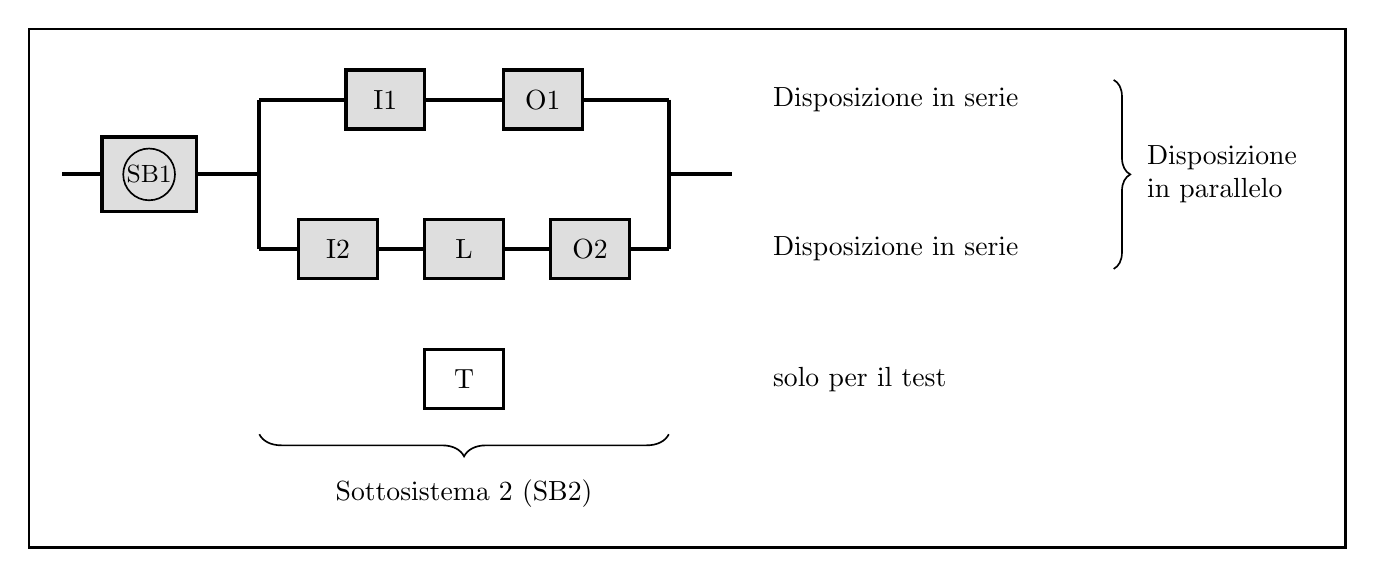
\begin{tikzpicture}[
  font=\normalsize,
  blocco/.style={draw=black, fill=black!13, line width=1.2pt,
                 minimum width=1.0cm, minimum height=0.75cm, inner sep=1pt},
  linea/.style={draw=black, line width=1.4pt}
]

% ---- sottosistema SB1 --------------------------------------------------
\draw[linea] (-1.1,0) -- (1.4,0);
\node[blocco, minimum width=1.2cm, minimum height=0.95cm] (SB1) at (0,0) {};
\node[draw=black, fill=black!13, circle, line width=0.6pt, inner sep=0.5pt, font=\small] at (0,0) {SB1};

% ---- sottosistema SB2: due canali in parallelo ------------------------
\draw[linea] (1.4,0.95) -- (1.4,-0.95);
\draw[linea] (6.6,0.95) -- (6.6,-0.95);
\draw[linea] (6.6,0) -- (7.4,0);

\draw[linea] (1.4,0.95) -- (6.6,0.95);
\node[blocco] at (3.0,0.95) {I1};
\node[blocco] at (5.0,0.95) {O1};

\draw[linea] (1.4,-0.95) -- (6.6,-0.95);
\node[blocco] at (2.4,-0.95) {I2};
\node[blocco] at (4.0,-0.95) {L};
\node[blocco] at (5.6,-0.95) {O2};

\node[blocco, fill=white] at (4.0,-2.6) {T};

% ---- etichette ---------------------------------------------------------
\node[anchor=west] (s1) at (7.8,0.95)  {Disposizione in serie};
\node[anchor=west] (s2) at (7.8,-0.95) {Disposizione in serie};
\draw[line width=0.6pt, decorate, decoration={brace, amplitude=6pt}]
  (12.25,1.2) -- (12.25,-1.2);
\node[anchor=west, align=left] at (12.55,0) {Disposizione\\ in parallelo};
\node[anchor=west] at (7.8,-2.6) {solo per il test};

\draw[line width=0.6pt, decorate, decoration={brace, amplitude=8pt, mirror}]
  (1.4,-3.3) -- (6.6,-3.3);
\node at (4.0,-4.05) {Sottosistema 2 (SB2)};

% ---- cornice -------------------------------------------------------------
\draw[line width=1pt]
  ([shift={(-0.4,0.5)}]current bounding box.north west) rectangle
  ([shift={(0.5,-0.4)}]current bounding box.south east);

\end{tikzpicture}
}
        \captionof{figure}{Esempio generale di schema a blocchi legato alla sicurezza; I1 e O1 costituiscono il primo canale (disposizione in serie), mentre I2, L e O2 costituiscono il secondo (disposizione in serie); la funzione di sicurezza è eseguita in modo ridondante da entrambi i canali (disposizione in parallelo); T è utilizzato soltanto per il test.}
        \label{fig:06-09}
    \end{minipage}
\end{center}
Conformemente a questa definizione, per la rappresentazione di un sistema di comando legato alla sicurezza sotto forma di schema a blocchi legato alla sicurezza si possono formulare le seguenti regole:
•	la disposizione di blocchi in serie sotto forma di "canale" (es. blocchi I, L e O) esprime il fatto che il guasto di un blocco può portare al guasto dell'intera catena. Se, ad esempio, un'unità hardware di un canale si guasta in modo pericoloso, l'intero canale diventa incapace di eseguire la funzione di sicurezza;
•	una disposizione in parallelo di blocchi o canali simboleggia l'esecuzione ridondante multipla della funzione di sicurezza o di sue parti rilevanti. Ad esempio, una funzione di sicurezza eseguita da più canali è mantenuta purché almeno un canale non abbia subito un guasto;
•	i blocchi impiegati soltanto a scopo di test, il cui guasto non compromette l'esecuzione della funzione di sicurezza nei diversi canali, possono essere rappresentati come canale di test separato. Sebbene il guasto delle misure di test comporti una riduzione dell'affidabilità del sistema nel suo complesso, l'effetto è inizialmente solo di lieve entità, purché resti assicurata l'esecuzione della funzione di sicurezza vera e propria nei singoli canali.
La definizione dei blocchi e dei canali procede di pari passo con la determinazione della categoria, ed è il primo passo nella quantificazione del PL. Per questo scopo sono necessari ulteriori valori: la valutazione dell'affidabilità dei componenti (MTTF\textsubscript{D}), dei test (DC\textsubscript{avg}) e della rilevanza dei guasti per causa comune (CCF). Ulteriori informazioni sul percorso "dallo schema concettuale al Performance Level", in particolare sulla derivazione dello schema a blocchi legato alla sicurezza, si trovano nel SISTEMA Cookbook 1~\cite{cookbook1}. Questo cookbook introduce anche il termine "sottosistema incapsulato". Con questo termine si intende un sottosistema per il quale il fabbricante indica già PL, PFH\textsubscript{D} e categoria, e la cui struttura interna precisa e i cui parametri non sono trasparenti. Questi parametri dichiarati richiedono l'osservanza delle condizioni d'uso specificate dal fabbricante, che possono ad esempio includere la realizzazione di una diagnostica esterna. Esso viene rappresentato nello schema a blocchi legato alla sicurezza, a livello di sottosistema, in forma monocanale, come un cerchio all'interno di un blocco (vedere il sottosistema "SB1" nella Figura~\ref{fig:06-09}).

Esso contribuisce alla quantificazione del PL soltanto attraverso i propri parametri PFH\textsubscript{D} e PL\textsubscript{r} l'indicazione della categoria ha valore puramente informativo.

\subsection{Considerazioni sui guasti ed esclusione dei guasti}
\label{subsec:06-2-10}
In un sistema di comando reale, il numero di guasti teoricamente possibili non è in alcun modo limitato. La valutazione deve pertanto essere limitata ai guasti rilevanti. Alcuni guasti possono essere esclusi se si considerano i seguenti punti:
\begin{itemize}
    \item l'improbabilità tecnica del loro verificarsi (una probabilità inferiore di diversi ordini di grandezza rispetto a quella di altri guasti possibili e alla riduzione del rischio da conseguire);
    \item l'esperienza tecnica generalmente riconosciuta, indipendentemente dall'applicazione in esame;
    \item i requisiti tecnici relativi all'applicazione e al pericolo specifico;
\end{itemize}

I guasti dei componenti che possono verificarsi e quelli che possono essere esclusi sono descritti nella EN ISO 13849-2. Devono essere osservati i seguenti punti:
\begin{itemize}
    \item gli elenchi dei guasti costituiscono soltanto una selezione. Ove necessario, devono pertanto essere creati nuovi modelli di guasto (ad esempio per componenti nuovi), oppure devono essere considerati ulteriori tipi di guasto, a seconda dell'applicazione. Ciò può essere determinato, ad esempio, mediante un'analisi FMEA;
    \item i guasti secondari sono valutati come un unico guasto insieme al guasto iniziale che li ha originati, così come i guasti multipli con causa comune (CCF, guasti per causa comune);
    \item il verificarsi simultaneo di due o più guasti differenti per causa è considerato estremamente improbabile e non deve pertanto essere preso in considerazione;
\end{itemize}

Ulteriori informazioni sull'esclusione di guasto si trovano nell'Allegato~\ref{app:C} e nella Parte 2 della EN ISO 13849. Qualora vengano esclusi guasti senza che il motivo dell'esclusione sia immediatamente evidente (come il distacco delle piste su un layout di circuito stampato correttamente dimensionato), nella documentazione tecnica deve essere indicata una motivazione precisa. A condizione che siano soddisfatte le relative condizioni, le esclusioni di guasto sono possibili anche per i componenti, ad esempio per i contatti elettrici di apertura e per l'azionamento meccanico degli interruttori di posizione elettromeccanici o dei dispositivi di arresto di emergenza. La validità delle esclusioni di guasto può in questo caso essere limitata ai PL bassi; si rimanda ad esempio alla Tabella D.8 della EN ISO 13849-2 e all'Allegato~\ref{app:D} del presente rapporto. Se si applica l'esclusione di guasto, per tali componenti non è necessario considerare i tassi di guasto (MTTF\textsubscript{D}) né le misure di monitoraggio (DC).

\subsection{Tempo medio al guasto pericoloso}
\label{subsec:06-2-11}
L'affidabilità dei singoli componenti da cui è costruito il sistema di comando fornisce un contributo decisivo alla sua affidabilità complessiva. L'MTTF\textsubscript{D} (tempo medio al guasto pericoloso) è pertanto considerato nel PL come valore di affidabilità. È chiaro che in questo contesto "guasto" si riferisce ai difetti dei componenti che comportano il mancato o non più corretto svolgimento della funzione realizzata. Le altre parti del termine richiedono tuttavia una spiegazione:
\begin{itemize}
    \item "Medio" indica che il valore è una media statistica: esso non si riferisce a uno specifico componente, ma è definito come valore atteso per la vita media del componente tipico. In questo contesto, il valore atteso per un singolo componente può essere considerato uguale al valore medio di un elevato numero di componenti dello stesso tipo. Il valore non costituisce pertanto una durata di vita minima garantita nel senso di un periodo esente da guasti. Questo approccio basato su un valore medio si riflette anche nel fatto che i valori di durata di vita normalmente non vengono adattati alle condizioni d'impiego (es. carico, temperatura, clima), purché i componenti siano impiegati entro le condizioni d'impiego specificate per essi. Si presume generalmente, in questo caso, che il carico più elevato in un'applicazione di un dispositivo sia compensato, in media, da un carico più basso in un'altra applicazione. Qualora tuttavia carichi più elevati siano prevedibili in tutte le applicazioni (ad esempio a causa di temperature estreme), tali condizioni devono essere considerate nella determinazione dell'MTTF\textsubscript{D};
    \item "Tempo" indica che l'affidabilità è espressa in termini di un tempo nel senso di una durata di vita. L'MTTF\textsubscript{D} è generalmente indicato in anni (abbreviato "a"). Altre forme di notazione che possono essere convertite in un MTTF\textsubscript{D} comprendono i tassi di guasto o i cicli (di commutazione). I tassi di guasto sono generalmente indicati con la lettera greca minuscola λ (lambda) ed espressi nell'unità "FIT" (= 10⁻⁹/h, ossia guasti per miliardo di ore-componente). La relazione tra λ\textsubscript{D} e MTTF\textsubscript{D} è espressa, a tasso di guasto λ\textsubscript{D} costante nel corso della durata di vita, come MTTF\textsubscript{D} = 1/λ\textsubscript{D}. Occorre naturalmente considerare la conversione da ore ad anni. Per i componenti che si usurano principalmente a seguito del loro funzionamento meccanico, l'affidabilità è generalmente espressa in cicli di commutazione, ad esempio come valore B\textsubscript{10D}, ossia il numero medio di cicli fino a cui il 10\% dei componenti si guasta in modo pericoloso. L'MTTF\textsubscript{D} può in questo caso essere calcolato considerando il numero medio di manovre all'anno n\textsubscript{op} previste per l'applicazione in questione. Per maggiori dettagli si rimanda all'Allegato~\ref{app:D};
    \item "Pericoloso" indica che, ai fini del PL, vengono in ultima analisi considerati soltanto i guasti che compromettono l'esecuzione della funzione di sicurezza (guasto non sicuro). I guasti sicuri, al contrario, possono ben causare l'assunzione dello stato sicuro (inibizione del funzionamento) o ridurre la disponibilità o la produttività di una macchina, ma la funzione di sicurezza viene comunque eseguita correttamente, oppure lo stato sicuro viene comunque avviato/mantenuto. Nelle strutture ridondanti, tuttavia, l'attributo "pericoloso" si riferisce a ciascun singolo canale. Qualora un guasto in un canale renda inoperante la funzione di sicurezza, il guasto in questione è considerato pericoloso, anche laddove un ulteriore canale sia ancora in grado di eseguire con successo la funzione di sicurezza;
\end{itemize}

Un MTTF\textsubscript{D} può essere indicato sia per un singolo componente, come un transistor, una valvola o un contattore, sia per un blocco, un canale, o il sistema di comando nel suo complesso. Questo MTTF\textsubscript{D} complessivo rappresenta il valore per un canale, eventualmente simmetrizzato su più canali, e si basa sull'MTTF\textsubscript{D} di tutti i componenti coinvolti nella SRP/CS. Conformemente al principio bottom-up, l'unità in esame viene progressivamente ampliata. Ai fini della riduzione dell'impegno, è spesso vantaggioso considerare nell'analisi soltanto i componenti legati alla sicurezza, ossia i componenti il cui guasto potrebbe avere un'influenza negativa, diretta o indiretta, sull'esecuzione della funzione di sicurezza. Per semplificare, sono inoltre possibili esclusioni di guasto; queste tengono conto del fatto che alcuni guasti sono estremamente improbabili e il loro contributo all'affidabilità complessiva è trascurabile. L'assunzione di esclusioni di guasto è tuttavia subordinata a determinate condizioni, illustrate in dettaglio nella EN ISO 13849-2 e descritte più diffusamente al punto~\ref{subsec:06-2-10}. I cortocircuiti dei conduttori o alcuni guasti meccanici possono ad esempio essere esclusi sulla base della progettazione, purché siano soddisfatte determinate condizioni.

\subsection{Fonti di dati per i singoli componenti}
\label{subsec:06-2-12}
Una delle domande più frequentemente poste in questo contesto riguarda il reperimento di dati di guasto affidabili per i componenti legati alla sicurezza. A tale scopo dovrebbe essere data preferenza al fabbricante, e ad esempio alla sua scheda tecnica, rispetto a qualsiasi altra fonte. Numerosi fabbricanti, ad esempio di componenti elettromeccanici o pneumatici, rendono ormai disponibili tali informazioni. Qualora i dati non siano disponibili da parte del fabbricante, valori esemplificativi tipici possono comunque essere ricavati da banche dati consolidate (vedere Allegato~\ref{app:D}). Tali fonti generalmente non distinguono tra guasti pericolosi e guasti sicuri; si può tuttavia assumere, come approssimazione generale, che in media soltanto la metà di tutti i guasti sia pericolosa. Tenendo conto della problematica del reperimento dei valori di affidabilità, la EN ISO 13849-1 elenca una serie di valori tipici. Si tratta tuttavia di stime molto conservative, il cui impiego è pertanto raccomandato soltanto qualora le fonti di dati sopra indicate non siano disponibili. Oltre ai valori di MTTF\textsubscript{D} per i componenti meccanici, idraulici ed elettronici, la norma contiene anche valori di B\textsubscript{10D} per i componenti pneumatici ed elettromeccanici. I dettagli sono descritti nell'Allegato~\ref{app:D}.
Una comoda fonte di dati di affidabilità per componenti destinati all'impiego in sistemi di comando orientati alla sicurezza è costituita dal gran numero di librerie SISTEMA disponibili (vedere Allegato H). Queste contengono valori di MTTF\textsubscript{D} o B\textsubscript{10D} per elementi e componenti, e valori di PL e PFH\textsubscript{D} per interi sottosistemi.

\subsection{FMEA rispetto al metodo del conteggio dei componenti (parts count)}
\label{subsec:06-2-13}
Una volta ottenuti i valori di MTTF\textsubscript{D} di tutti i componenti legati alla sicurezza, alcune semplici regole possono essere utilizzate per calcolare a partire da essi il valore di MTTF\textsubscript{D} del sistema di comando. A tale scopo possono essere impiegati diversi metodi: in modo complesso, mediante un'analisi precisa dei modi di guasto e dei loro effetti (FMEA), oppure in modo rapido e semplice mediante il metodo del conteggio dei componenti (parts count), che comporta lievi stime a favore della sicurezza. Il punto di partenza è la piccola differenza tra MTTF e MTTF\textsubscript{D}: quale proporzione dei guasti di un determinato componente è pericolosa? In una FMEA complessa possono essere elencati tutti i modi di guasto concepibili, valutati come "sicuri" o "pericolosi", e stimata la frazione della loro incidenza. Poiché gli effetti del guasto di un componente sul blocco determinano se il modo di guasto sia sicuro o pericoloso, possono rendersi necessarie analisi dettagliate dell'effetto causato da un guasto. Un numero maggiore di modi di guasto può in tal caso risultare "sicuro" rispetto a quanto avviene con una valutazione semplificata, come quella proposta dalla EN ISO 13849-1: se si utilizza il metodo del conteggio dei componenti, il suo approccio conservativo assume che, nel complesso, i guasti sicuri e quelli pericolosi siano simili per numero. In assenza di informazioni più dettagliate, con questo metodo si assume pertanto sempre che l'MTTF\textsubscript{D} sia il doppio dell'MTTF.
Anche in questo caso vale il principio della media statistica, ossia una valutazione eccessivamente favorevole di un componente è compensata da una valutazione troppo pessimistica di un altro. È del tutto possibile combinare il metodo del conteggio dei componenti con una FMEA. Laddove i valori prodotti dal solo conteggio dei componenti diano luogo a un PFH sufficientemente basso, non è necessario eseguire una FMEA. Qualora ciò non avvenga, tuttavia, è vantaggioso uno studio dei modi di guasto, ad esempio mediante una FMEA parziale, in particolare sui componenti che presentano i valori di MTTF\textsubscript{D} peggiori. Ulteriori spiegazioni su questo argomento si trovano nell'Allegato~\ref{app:B}.

Come per altri metodi di quantificazione, la valutazione secondo la EN ISO 13849-1 assume, per tutti i valori di MTTF\textsubscript{D}, un tasso di guasto costante durante l'intero tempo di missione del componente. Anche se ciò non rispecchia direttamente il comportamento al guasto, come ad esempio nel caso dei componenti soggetti a forte usura, in questo modo viene comunque determinato, mediante una stima a favore della sicurezza, un valore approssimativo di MTTF\textsubscript{D} che resta valido per l'intero tempo di missione del componente. I guasti precoci sono generalmente trascurati, poiché i componenti che presentano marcati andamenti di guasto precoce non soddisfano i requisiti di disponibilità di un sistema di comando di macchina e pertanto non sono generalmente significativi sul mercato. Il vantaggio di questa procedura è che l'MTTF\textsubscript{D} risulta sempre pari al reciproco del corrispondente tasso di guasto pericoloso λ\textsubscript{D}. Poiché i tassi di guasto pericoloso λ\textsubscript{D} dei componenti di un blocco possono essere semplicemente sommati tra loro, i valori di MTTF\textsubscript{D} dei componenti coinvolti (N componenti con indice corrente i) danno origine all'MTTF\textsubscript{D} del blocco come segue:
\begin{equation}
    \uplambda_{\mathrm{D}} = \sum_{i=1}^{N} \uplambda_{\mathrm{D}i}
    \quad\text{ovvero}\quad
    \frac{1}{\textit{MTTF}_{\mathrm{D}}} = \sum_{i=1}^{N} \frac{1}{\textit{MTTF}_{\mathrm{D}i}}
    \label{eq:06-01}
\end{equation}

La stessa relazione si applica al calcolo dell'MTTF\textsubscript{D} di ciascun canale a partire dai valori di MTTF\textsubscript{D} dei blocchi associati. Una volta noto l'MTTF\textsubscript{D} di ciascun canale, viene effettuata un'ulteriore semplificazione sotto forma di classificazione. I valori calcolati vengono assegnati a tre classi tipiche (Tabella~\ref{tab:06-3}).

\begin{table}[ht]
    \centering
    \definecolor{tabblue}{RGB}{31,73,125}
    \setlength{\tabcolsep}{4pt}
    \renewcommand{\arraystretch}{1.2}
    \caption{Classificazione dell'\textit{MTTF}\textsubscript{D} di ciascun canale.}
    \label{tab:06-3}
    \begin{tabularx}{\textwidth}{|>{\raggedright\arraybackslash}p{5.2cm}|X|}
        \hline
        \rowcolor{tabblue}
        \multicolumn{2}{|c|}{\textcolor{white}{\textbf{\textit{MTTF}\textsubscript{D} di ciascun canale}}} \\
        \rowcolor{tabblue}
        \textcolor{white}{\textbf{Descrizione}} &
        \multicolumn{1}{c|}{\textcolor{white}{\textbf{Intervallo}}} \\
        \hline
        Non adatto & 0~anni $\leq$ \textit{MTTF}\textsubscript{D} $<$ 3~anni \\
        \hline
        \rowcolor{black!8}
        Basso & 3~anni $\leq$ \textit{MTTF}\textsubscript{D} $<$ 10~anni \\
        \hline
        Medio & 10~anni $\leq$ \textit{MTTF}\textsubscript{D} $<$ 30~anni \\
        \hline
        \rowcolor{black!8}
        Alto & 30~anni $\leq$ \textit{MTTF}\textsubscript{D} $\leq$ 100~anni \\
        \hline
        Ammesso soltanto nella categoria 4 & 100~anni $<$ \textit{MTTF}\textsubscript{D} $\leq$ 2.500~anni \\
        \hline
    \end{tabularx}
\end{table}

Un tempo medio (importante: non garantito) di vita inferiore a tre anni è considerato non ragionevole per componenti di sicurezza. Ad eccezione della Categoria 4, i valori superiori a 100 anni non possono essere sostituiti; ciò impedisce che l'affidabilità del componente venga sopravvalutata rispetto alle altre principali variabili di influenza, quali la struttura o i test. Qualora per un canale risultasse effettivamente un valore inferiore a tre anni, i componenti dovrebbero essere sostituiti con alternative più affidabili, poiché altrimenti non sarebbe raggiungibile nemmeno il PL a. Valori superiori a 100 anni per il tempo medio di vita non sono infrequenti, ma a causa del "capping" non hanno alcuna influenza sul PL al di sopra di tale valore, poiché in questo caso viene sostituito, ai fini dell'affidabilità del componente, il valore massimo di 100 anni (il valore massimo in Categoria 4 è 2.500 anni).
Se in un sistema di comando sono coinvolti più canali, non è immediatamente chiaro quale valore debba essere impiegato come rappresentativo per l'intero sistema. Un approccio cautelativo consisterebbe naturalmente nell'assumere il valore più basso; risultati migliori, pur rimanendo dal lato della sicurezza, sono tuttavia ottenuti mediante la seguente formula di media (C1 e C2 si riferiscono qui ai due canali, che vengono simmetrizzati):
\begin{equation}
    \textit{MTTF}_{\mathrm{D}} = \frac{2}{3}
    \left( \textit{MTTF}_{\mathrm{DC1}} + \textit{MTTF}_{\mathrm{DC2}}
    - \frac{1}{\dfrac{1}{\textit{MTTF}_{\mathrm{DC1}}} + \dfrac{1}{\textit{MTTF}_{\mathrm{DC2}}}} \right)
    \label{eq:06-02}
\end{equation}

Qualora i canali interessati siano bilanciati, il valore di MTTF\textsubscript{D} così calcolato corrisponde al valore di MTTF\textsubscript{D} di un singolo canale. Qualora essi siano sbilanciati, il risultato è un MTTF\textsubscript{D} medio che non può essere inferiore ai due terzi del valore migliore. In questo scenario può inoltre verificarsi l'effetto per cui il valore migliore era stato precedentemente sottoposto a capping a un MTTF\textsubscript{D} di 100 anni (2.500 anni nel caso della Categoria 4), e di conseguenza il valore simmetrizzato risulta inferiore a 100 anni (2.500 anni per la Categoria 4). È pertanto generalmente più efficace realizzare, ove possibile, canali di affidabilità bilanciata. Indipendentemente dal numero e dalla forma dei canali, questo metodo produce sempre un valore di MTTF\textsubscript{D} per un singolo canale di comando che, mediato sull'intero sistema di comando, indica il livello di affidabilità dei componenti.

\subsection{Copertura diagnostica delle misure di test e monitoraggio}
\label{subsec:06-2-14}
Un'ulteriore variabile con un'influenza rilevante sul PL sono le misure di (auto)test e monitoraggio nell'SRP/CS. Test efficaci, ad esempio, consentono di compensare in parte una scarsa affidabilità dei componenti. La qualità dei test viene misurata, nella EN ISO 13849-1, mediante la copertura diagnostica (DC). La DC è definita come la proporzione di guasti pericolosi rilevati rispetto a tutti i guasti pericolosi concepibili. La grandezza di riferimento può essere un componente, un blocco, oppure l'intero SRP/CS. In quest'ultimo caso, la DC corrisponde alla copertura diagnostica media DC\textsubscript{avg}, che svolge una funzione importante nella quantificazione semplificata del PL mediante il metodo del diagramma a barre.

Come in molti altri punti della norma, esistono due metodi per il calcolo della DC\textsubscript{avg}: uno più preciso ma più complesso; l'altro più semplice, basato su una serie di stime a favore della sicurezza. Il metodo preciso e complesso prevede un'analisi dei modi di guasto e dei loro effetti (FMEA) e si basa sulla definizione di DC. In questo caso vengono determinati, per ciascun componente, i modi di guasto pericolosi rilevabili (DD) e pericolosi non rilevabili (DU), unitamente alle rispettive proporzioni rispetto al tasso di guasto totale del componente. Infine, mediante sommatoria e formazione del rapporto, si ottiene il valore di DC per l'unità considerata:
\begin{equation}
    \textit{DC} = \frac{\displaystyle\sum \uplambda_{\mathrm{DD}}}{\displaystyle\sum \uplambda_{\mathrm{DD}} + \sum \uplambda_{\mathrm{DU}}}
    = \frac{\displaystyle\sum \uplambda_{\mathrm{DD}}}{\displaystyle\sum \uplambda_{\mathrm{D}}}
    \label{eq:06-03}
\end{equation}

Il metodo privilegiato dalla EN ISO 13849-1 si basa su una stima cautelativa e motivata della DC direttamente a livello di componente o di blocco, seguita dal calcolo della DC\textsubscript{avg} a partire dai singoli valori di DC mediante una formula di media. Molti test possono essere classificati come misure tipiche standard, per le quali valori di DC stimati sono riportati nell'Allegato E della norma. A tali misure viene assegnato un sistema semplificato comprendente quattro valori chiave (0\%, 60\%, 90\% e 99\%). Un elenco completo delle misure di test tipiche indicate nella norma è disponibile nell'Allegato E. L'applicazione viene illustrata con riferimento all'esempio del sistema di comando di una taglierina per carta a ghigliottina (cfr. sottoparagrafo 6.5).
Per il calcolo della DC di un componente o di un blocco devono essere osservate alcune condizioni al contorno:
\begin{itemize}
    \item la rilevazione di un guasto pericoloso è solo l'inizio. Affinché il test possa dirsi superato, deve essere tempestivamente avviato uno stato di sicurezza che non presenti ulteriori pericoli. Questo comporta un percorso di disinserzione efficace, che ad esempio, nel caso di sistemi monocanale testati (Categoria 2), comporta il requisito di un secondo elemento di disinserzione. Ciò è necessario per avviare e mantenere lo stato di sicurezza quando il test ha rilevato il guasto dell'elemento di disinserzione normale (blocco "O" nello schema a blocchi correlato alla sicurezza). Solo quando il rischio è basso (fino a PL\textsubscript{r} = c) e quando l'avvio di uno stato di sicurezza non è possibile (ad esempio a causa della saldatura dei contatti del dispositivo di commutazione finale) può essere sufficiente, in Categoria 2, che l'uscita dell'apparecchiatura di test (OTE) fornisca soltanto un avviso.
    \item l'avvio di un test, la sua esecuzione e il necessario processo di disinserzione dovrebbero idealmente essere eseguiti automaticamente dall'SRP/CS. Solo in casi eccezionali è accettabile fare affidamento, in questo contesto, sull'intervento manuale, ad esempio da parte dell'operatore della macchina, poiché l'esperienza pratica dimostra che le misure necessarie spesso non vengono adeguatamente attuate, sia per pigrizia, sia a causa della pressione lavorativa o di una scarsa informazione od organizzazione. L'attuazione efficace dei test manuali comporta un maggiore coinvolgimento nel processo di lavoro, ovvero un maggiore impegno organizzativo e disciplina. Il calcolo della DC tiene comunque conto della rilevazione dei guasti quando viene fatta una richiesta alla funzione di sicurezza, ossia la considerazione non si limita ai test avviati automaticamente da elettronica programmabile; i componenti elettromeccanici come relè o contattori costituiscono casi classici in cui il guasto di "mancata diseccitazione" può tipicamente essere rilevato solo quando viene fatta una richiesta alla funzione di sicurezza. Laddove i guasti debbano essere rilevati in occasione di una richiesta, occorre considerare la frequenza con cui viene fatta una richiesta alla funzione di sicurezza, al fine di garantire una frequenza di test adeguata, come descritto nel punto successivo;
    \item un ulteriore aspetto riguarda la questione della frequenza di test necessaria. Un test che non viene eseguito con frequenza sufficiente può, in determinate circostanze, essere superato dall'insorgere di un evento pericoloso, e può pertanto creare un falso senso di sicurezza. Come regola empirica, la frequenza di test è sempre in competizione con altre frequenze; per questo motivo non è possibile indicare una frequenza adeguata di validità generale. Inoltre, i test hanno la funzione di rivelare non solo guasti casuali, ma anche guasti sistematici;
\end{itemize}

Nei sistemi monocanale testati di Categoria 2, il test deve essere superato prima che venga fatta la richiesta successiva alla funzione di sicurezza, ossia prima che insorga un potenziale pericolo. In questo scenario, la frequenza di test è pertanto in competizione con la frequenza di richiesta della funzione di sicurezza. In questo caso, un fattore pari a 100 è considerato sufficiente, ossia una frequenza di test almeno 100 volte superiore alla frequenza media di richiesta della funzione di sicurezza. Per contro, fino a un fattore pari a 25, l'incremento massimo della probabilità di guasto è di circa il 10\% (cfr. anche il sottoparagrafo 4 in~\cite{cookbook4}). Al di sotto di questo livello, è essenzialmente la sincronizzazione tra richiesta e test a determinare se il test abbia effettivamente efficacia. Qualora, nei sistemi monocanale testati, il test venga eseguito simultaneamente alla richiesta della funzione di sicurezza e in modo così rapido che lo stato di sicurezza venga raggiunto prima che insorga un pericolo, non viene imposta alcuna condizione sulla frequenza di test. (Ciò vale — con riferimento alle raccomandazioni indicate di seguito per la frequenza di test nei sistemi a due canali — a condizione che si possa presumere almeno una richiesta all'anno.) Un esempio particolare è costituito dal test continuo (ad es. monitoraggio analogico di sovratensione/sottotensione), per il quale i requisiti relativi alla frequenza di test sono sempre soddisfatti quando lo stato di sicurezza viene raggiunto con sufficiente rapidità.

Nei sistemi a due canali di Categoria 3 e 4, la frequenza di test è in competizione con la frequenza di insorgenza di un secondo guasto pericoloso, poiché solo se il secondo canale si guasta prima che un test abbia rilevato il guasto del primo canale sussiste il pericolo che la funzione di sicurezza non venga eseguita. Per definizione, i sistemi di Categoria 4 tollerano persino l'accumulo di guasti non rilevati. Nella pratica esiste una serie di raccomandazioni per la frequenza di test minima necessaria nelle Categorie 3 e 4.

La norma IEC 61800-5-2~\cite{iec61800-5-2}, relativa alla sicurezza dei sistemi di azionamento elettrico di potenza, considera accettabili le seguenti frequenze minime di test diagnostico per il caso in cui il test non possa essere eseguito senza interruzione del ciclo di lavoro della macchina e in cui non sia attuabile alcuna soluzione tecnica ragionevole: un test all'anno per il PL d in Categoria 3, un test ogni tre mesi per il PL e in Categoria 3, e un test al giorno per il PL e in Categoria 4.

Nella EN ISO 14119~\cite{eniso14119} e in una "Raccomandazione per l'uso" degli organismi notificati del settore macchine~\cite{rfu2015}, per le uscite elettromeccaniche (relè o contattori) è richiesto un test automatico o manuale ai seguenti intervalli: almeno una volta al mese per il PL e in Categoria 3 o 4, e almeno una volta ogni dodici mesi per il PL d in Categoria 3. Il test dovrebbe preferibilmente essere eseguito in modo automatico; in alternativa, l'intervallo di test può essere monitorato automaticamente. Solo in casi eccezionali dovrebbe essere garantito mediante misure organizzative.

Le frequenze di test qui indicate sono requisiti minimi, applicabili quando test più frequenti non sono possibili, ad esempio perché il test può essere eseguito solo quando viene fatta una richiesta alla funzione di sicurezza (per la quale è necessaria una variazione di segnale, come ad esempio nel caso della tecnologia elettromeccanica o fluidica), oppure perché è richiesta un'interruzione del ciclo di lavoro della macchina, come ad esempio all'avvio della macchina all'inizio del turno. I test automatici che non sono soggetti a tali vincoli, come i test del processore o della memoria nei sistemi elettronici, possono spesso essere implementati con una frequenza notevolmente superiore senza un onere significativo. In questi casi, nella pratica si è dimostrato adeguato un test almeno una volta per turno per la Categoria 3; nella Categoria 4, una frequenza minima di test pari a una volta all'ora era già stata scelta quando era in vigore la norma precedente EN 954-1.

\begin{itemize}
    \item un ulteriore aspetto è l'affidabilità della stessa apparecchiatura di test. A questo proposito, la norma stabilisce solo i requisiti di base della Categoria B, applicabili a tutte le Categorie, ossia la conformità alle norme pertinenti affinché le influenze previste possano essere sopportate, e l'applicazione di principi di sicurezza fondamentali. Nella misura del possibile, dovrebbero inoltre essere applicati principi di sicurezza collaudati. Laddove i guasti pericolosi dell'apparecchiatura di test vengano rilevati mediante la sua incorporazione ciclica nel processo, è ammessa una deroga a tali requisiti di base. Un ulteriore requisito generale è che l'apparecchiatura di test non debba guastarsi prima dei componenti che essa monitora. Allo stesso tempo, non è efficiente investire nell'affidabilità dell'apparecchiatura di test molto più di quanto si investa nell'apparecchiatura di sicurezza che esegue propriamente la funzione di sicurezza. La EN ISO 13849-1 impone pertanto solo requisiti limitati sull'affidabilità dell'apparecchiatura di test. Per le Categorie 3 e 4, ci si affida alla tolleranza al guasto singolo, poiché, includendo il guasto dell'apparecchiatura di test, devono verificarsi complessivamente tre guasti pericolosi prima che la funzione di sicurezza cessi di essere eseguita. Il verificarsi inosservato di un tale caso è considerato estremamente improbabile e pertanto non critico. Per la Categoria 2 esiste una condizione secondaria — quantomeno con la procedura semplificata di determinazione del PL mediante il diagramma a barre — stabilita durante il calcolo delle "barre di Categoria 2": in questo caso, il tasso di guasto pericoloso del canale di test non dovrebbe superare il doppio del tasso di guasto pericoloso del canale funzionale che esso monitora.
    \item l'efficacia di una determinata misura di test, ad esempio la rilevazione dei guasti da parte del processo, può dipendere in misura significativa dall'applicazione, e può variare tra 0 e 99\%. In questo caso occorre prestare particolare attenzione nella scelta di uno dei valori chiave della DC. Ulteriori spiegazioni sono disponibili nell'Allegato E.
    \item i finecorsa di posizione collegati in serie, ove presenti, devono essere presi in considerazione nella determinazione del valore DC\textsubscript{avg} per i contatti elettromeccanici. In tali casi può verificarsi un mascheramento dei guasti, che richiede una riduzione del valore DC\textsubscript{avg} e del PL raggiungibile. I dettagli sono disponibili nell'Allegato E.
    \item è possibile che componenti o blocchi siano monitorati da più test, oppure che test diversi agiscano su componenti diversi, con la conseguenza che deve essere determinata una DC complessiva per il componente o per il blocco. L'Allegato E fornisce indicazioni utili su queste problematiche.
    \item La formula~\eqref{eq:06-04} della DC\textsubscript{avg} fornisce un metodo di calcolo in cui blocchi con valori di DC diversi vengono raggruppati in modo tale che i requisiti minimi di DC\textsubscript{avg} per la Categoria raggiunta siano soddisfatti, anche se singoli blocchi presentano una DC inferiore al 60\%, o persino nessuna diagnostica (DC = 0\%). In tali casi, deve essere stabilito caso per caso se questa forma di implementazione sia coerente con i requisiti della Categoria. La Categoria 3 richiede ad esempio che, ove ragionevolmente possibile, un guasto singolo debba essere rilevato entro la successiva richiesta della funzione di sicurezza. Per la Categoria 2, un "controllo della funzione di sicurezza" costituisce un requisito generico. Anche la Categoria 4 richiede la rilevazione del singolo guasto, e solo "qualora tale rilevazione non sia possibile" che la funzione di sicurezza venga comunque eseguita in caso di accumulo di guasti non rilevati;
    \item per quanto riguarda in particolare i sistemi elettronici programmabili, è concepibile un numero elevato di guasti complessi; corrispondenti requisiti devono pertanto essere posti anche sulla complessità dei test. In questo caso, qualora sia richiesta una DC superiore al 60\% per la logica (programmabile o complessa), la EN ISO 13849-1 richiede almeno una misura per la memoria variabile, per la memoria non variabile e per l'unità di elaborazione — ove presenti — con una DC pari almeno al 60\% in ciascun caso.
\end{itemize}

Una volta noti i valori di DC di tutti i blocchi, il valore di DC\textsubscript{avg} per il sistema viene calcolato mediante la formula approssimata~\eqref{eq:06-04}. Questa formula pondera i singoli valori di DC con i rispettivi valori di MTTF\textsubscript{D}, poiché le parti molto affidabili (con un MTTF\textsubscript{D} elevato) dipendono meno da test efficaci rispetto alle parti meno affidabili (le sommatorie a numeratore e denominatore vengono formate su N blocchi dell'intero sistema):
\begin{equation}
    \textit{DC}_{\mathrm{avg}} =
    \frac{\dfrac{\textit{DC}_1}{\textit{MTTF}_{\mathrm{D1}}} + \dfrac{\textit{DC}_2}{\textit{MTTF}_{\mathrm{D2}}} + \ldots + \dfrac{\textit{DC}_N}{\textit{MTTF}_{\mathrm{D}N}}}
         {\dfrac{1}{\textit{MTTF}_{\mathrm{D1}}} + \dfrac{1}{\textit{MTTF}_{\mathrm{D2}}} + \ldots + \dfrac{1}{\textit{MTTF}_{\mathrm{D}N}}}
    \label{eq:06-04}
\end{equation}

Una volta ottenuto, il valore di DC\textsubscript{avg} rappresenta un valore che descrive la qualità delle misure di test e monitoraggio mediata sull'intero SRP/CS. Prima che questo valore possa essere sostituito nella quantificazione semplificata del PL, insieme alla Categoria (cinque classi) e all'MTTF\textsubscript{D} di ciascun canale (tre classi), esso deve essere assegnato a una delle quattro classi della Tabella~\ref{tab:06-4}.

% Tabella non fluttuante (minipage + \captionof): a fine capitolo un float
% finirebbe da solo su una pagina a parte
\begin{center}
    \begin{minipage}{\textwidth}
    \captionsetup{hypcap=false}
    \definecolor{tabblue}{RGB}{31,73,125}
    \setlength{\tabcolsep}{4pt}
    \renewcommand{\arraystretch}{1.2}
    \captionof{table}{Le quattro classi di copertura diagnostica secondo l'approccio semplificato della EN~ISO~13849-1.}
    \label{tab:06-4}
    \begin{tabularx}{\textwidth}{|>{\raggedright\arraybackslash}p{5.2cm}|>{\centering\arraybackslash}X|}
        \hline
        \rowcolor{tabblue}
        \multicolumn{2}{|c|}{\textcolor{white}{\textbf{Copertura diagnostica (\textit{DC})}}} \\
        \rowcolor{tabblue}
        \textcolor{white}{\textbf{Descrizione}} &
        \textcolor{white}{\textbf{Intervallo}} \\
        \hline
        Nessuna & \textit{DC} $<$ 60\% \\
        \hline
        \rowcolor{black!8}
        Bassa & 60\% $\leq$ \textit{DC} $<$ 90\% \\
        \hline
        Media & 90\% $\leq$ \textit{DC} $<$ 99\% \\
        \hline
        \rowcolor{black!8}
        Alta & 99\% $\leq$ \textit{DC} \\
        \hline
    \end{tabularx}
    \end{minipage}
\end{center}

Quando la DC\textsubscript{avg} viene successivamente utilizzata nella quantificazione semplificata mediante il diagramma a barre (cfr. sottoparagrafo 6.2.16), viene impiegato solo il rispettivo valore chiave inferiore della classe di DC\textsubscript{avg} (0, 60, 90 o 99). Anche in questo caso interviene quindi un'ulteriore semplificazione, basata su una stima a favore della sicurezza.

In casi specifici, tuttavia, questo sistema semplificato in modo grossolano può dare origine a paradossi, qualora ad esempio un componente poco affidabile con una DC superiore alla media per l'SRP/CS venga sostituito con un componente più affidabile (per una spiegazione più dettagliata, cfr. la fine dell'Allegato G).

\subsection{Misure dei guasti di causa comun(CCF)}
\label{subsec:06-2-15}
L'ultimo parametro rilevante per la quantificazione semplificata della probabilità di guasto riguarda i guasti di causa comune (CCF). Tali guasti sono guasti pericolosi correlati, presenti ad esempio in entrambi i canali di un SRP/CS ridondante, attribuibili a una causa comune. Esempi includono condizioni ambientali sfavorevoli o sovraccarichi non adeguatamente considerati durante la progettazione del sistema di comando. Qualora i canali non siano adeguatamente separati, possono verificarsi guasti secondari pericolosi che rendono inefficace la tolleranza al guasto singolo prevista. La rilevanza quantitativa di tali effetti in uno specifico sistema è difficile da stimare (cfr. anche l'Allegato F). Nell'Allegato D della IEC 61508-6 [37], per questo scopo viene utilizzato il modello del "fattore beta". In questo modello, il tasso di guasto di causa comune viene posto, come β · λ\textsubscript{D}, in relazione al tasso di guasto pericoloso di un canale λ\textsubscript{D}. Senza una FMEA precisa, tuttavia, β può essere al massimo solo stimato per un SRP/CS reale. A tale scopo, la EN ISO 13849-1 contiene una checklist di otto importanti contromisure, per le quali vengono assegnati punteggi compresi tra 5 e 25:
\begin{itemize}
    \item separazione fisica tra i percorsi di segnale dei diversi canali (15 punti);
    \item diversità nella tecnologia, nella progettazione o nei principi fisici dei canali (20 punti);
    \item protezione contro possibili sovraccarichi (15 punti);
    \item impiego di componenti collaudati (5 punti);
    \item analisi dei modi di guasto e dei loro effetti durante lo sviluppo, per l'identificazione di potenziali guasti di causa comune (5 punti);
    \item formazione dei progettisti/manutentori sui CCF e sulla loro prevenzione (5 punti);
    \item protezione contro i guasti di causa comune innescati da contaminazione (sistemi meccanici e fluidici) e da interferenze elettromagnetiche (sistemi elettrici) (25 punti);
    \item protezione contro i guasti di causa comune innescati da condizioni ambientali sfavorevoli (10 punti);
\end{itemize}

I punti indicati per una determinata contromisura devono essere assegnati per intero, oppure per niente; non vengono assegnati punti per un'attuazione "parziale" delle contromisure. Diversi pacchetti di misure possono tuttavia risultare efficaci contro i CCF a livello di sottosistema. Qualora tutte e otto le contromisure siano soddisfatte, viene assegnato un punteggio totale massimo di 100 punti. Tuttavia, la EN ISO 13849-1 richiede solo un punteggio totale minimo di 65 punti, e comunque solo per gli SRP/CS in Categoria 2, 3 e 4. Nei sistemi di Categoria 2, l'obiettivo è evitare guasti di causa comune pericolosi nei canali di test e funzionale che potrebbero dare origine a un'occorrenza non rilevata di un guasto pericoloso. Durante la creazione del diagramma a barre per la quantificazione semplificata, i 65 punti sono stati equiparati a un fattore beta del 2\%. L'approssimazione grossolana relativa alle cinque Categorie e alle tre classi di MTTF\textsubscript{D} e quattro di DC\textsubscript{avg} è stata ulteriormente estesa e ridotta a una semplice decisione sì/no. Mentre i benefici di una struttura ridondante vengono pressoché completamente annullati già a un fattore beta del 10\% o superiore, un fattore beta non superiore al 2\% riduce la rilevanza dei guasti di causa comune a un livello giustificabile.

\subsection{Determinazione semplificata del PL mediante il diagramma a barre}
\label{subsec:06-2-16}
Anche quando i quattro parametri quantitativi essenziali per il calcolo della probabilità di guasto sono stati determinati, la determinazione del PL raggiunto per l'SRP/CS a partire da essi resta comunque un compito complesso. Sebbene in linea di principio sia ammesso qualsiasi metodo idoneo, la EN ISO 13849-1 propone un metodo grafico semplice, basato su calcoli più complessi e su stime a favore della sicurezza: il metodo del diagramma a barre (cfr. Figura~\ref{fig:06-10}).

% La minipage tiene insieme disegno e didascalia (figura non fluttuante)
\begin{center}
    \begin{minipage}{\textwidth}
        \centering
        \captionsetup{hypcap=false}
        \resizebox{0.9\textwidth}{!}{%==============================================================
%  Figura 6.10 - Diagramma a barre per la determinazione
%  semplificata del PL
%  Adattamento in italiano della Figura 6.10 dell'IFA Report 2/2017
%
%  Le coordinate sono state ricavate dalla grafica vettoriale
%  dell'originale (pagina 61 di rep0217e.pdf) e sono espresse nei
%  punti PostScript di quel disegno; l'unita' della tikzpicture
%  (x=y=0.042cm) riporta il tutto alle proporzioni originali.
%
%  Sistema di riferimento: l'origine e' l'angolo in basso a sinistra
%  del riquadro del grafico; l'asse y e' rivolto verso l'alto.
%  Le sei linee orizzontali (da 10^-4 a 10^-8) sono equidistanti,
%  cioe' la scala delle PFHD e' logaritmica a tratti: ogni banda
%  corrisponde a un Performance Level (a ... e).
%==============================================================
\begin{tikzpicture}[
  x=0.042cm, y=0.042cm,
  font=\small,
  cornice/.style={draw=black, line width=0.9pt},
  riquadro/.style={draw=black, line width=1.06pt},
  griglia/.style={draw=black, line width=1.06pt,
                  dash pattern=on 4.24pt off 2.12pt},
  tacca/.style={draw=black, line width=1.06pt},
  separatore/.style={draw=black, line width=0.8pt},
  contorno/.style={draw=black, line width=0.8pt},
  puntini/.style={draw=black, line width=0.52pt, line cap=butt,
                  dash pattern=on 0.53pt off 1.05pt},
  tratti/.style={draw=black, line width=0.52pt},
  etichetta/.style={draw=black, fill=black!15, line width=1.06pt,
                    rounded corners=2.9pt, inner sep=0pt, align=center}
]

\setstretch{1}

% --- riempimenti delle barre ------------------------------------------
% MTTFD basso: fondo bianco a puntini (righe orizzontali tratteggiate)
\def\riempipuntini#1#2#3#4{%
  \begin{scope}
    \clip (#1,#2) rectangle (#3,#4);
    \foreach \k in {0,...,20}{%
      \draw[puntini] (#1,{#4-1.1-2.2155*\k}) -- (#3,{#4-1.1-2.2155*\k});}
  \end{scope}}
% MTTFD medio: fondo bianco con tratteggio a 45 gradi
\def\riempitratti#1#2#3#4{%
  \begin{scope}
    \clip (#1,#2) rectangle (#3,#4);
    \foreach \k in {0,...,34}{%
      \draw[tratti] (#1,{#2-(#4-#2)+3.13*\k})
        -- ++({(#3-#1)+(#4-#2)},{(#3-#1)+(#4-#2)});}
  \end{scope}}
\def\barrabassa#1#2#3#4{%
  \fill[white] (#1,#2) rectangle (#3,#4);
  \riempipuntini{#1}{#2}{#3}{#4}
  \draw[contorno] (#1,#2) rectangle (#3,#4);}
\def\barramedia#1#2#3#4{%
  \fill[white] (#1,#2) rectangle (#3,#4);
  \riempitratti{#1}{#2}{#3}{#4}
  \draw[contorno] (#1,#2) rectangle (#3,#4);}
\def\barraalta#1#2#3#4{%
  \fill[black] (#1,#2) rectangle (#3,#4);
  \draw[contorno] (#1,#2) rectangle (#3,#4);}

% --- colonna delle PFHD a sinistra --------------------------------------
\draw[black!15, line width=6.62pt] (-38.64,211.73) -- (-38.64,0.44);

\node[etichetta, minimum width=1.4423cm, minimum height=1.1726cm]
  at (-38.81,218.58) {\textit{PFH}$_{\mathrm{D}}$\\(1/h)};

% tacche + etichette dei valori (le sei linee orizzontali del grafico)
\foreach \yv/\testo in {175.89/{$10^{-4}$}, 140.50/{$10^{-5}$},
                        105.15/{$3\cdot 10^{-6}$}, 70.05/{$10^{-6}$},
                        34.87/{$10^{-7}$}, 0/{$10^{-8}$}}{%
  \draw[tacca] (-23.86,\yv) -- (-2.81,\yv);
  \node[etichetta, minimum width=1.4423cm, minimum height=0.5586cm]
    at (-38.81,\yv) {\testo};}

% --- asse dei PL ---------------------------------------------------------
\node at (-10.4,217.7) {PL};
\draw[draw=black, line width=1.06pt, -{Triangle[length=11pt,width=6pt]}]
  (0.03,-41.87) -- (0.03,208.69);
\foreach \yv/\pl in {158.2/a, 122.8/b, 87.6/c, 52.5/d, 17.4/e}
  \node at (-9.0,\yv) {\pl};

% --- riquadro del grafico e griglia --------------------------------------
\draw[riquadro] (0,0) rectangle (342.01,175.89);
\foreach \yv in {140.50, 105.15, 70.05, 34.87}
  \draw[griglia] (0.05,\yv) -- (342.03,\yv);

% --- barre ----------------------------------------------------------------
% Cat. B, DCavg = nessuna
\barrabassa{13.85}{143.10}{35.23}{160.84}
\barramedia{13.85}{111.48}{35.23}{143.10}
% Cat. 1, DCavg = nessuna
\barraalta{62.57}{74.80}{83.95}{111.08}
% Cat. 2, DCavg = bassa
\barrabassa{111.69}{130.62}{133.07}{155.26}
\barramedia{111.69}{92.81}{133.07}{130.62}
\barraalta{111.69}{60.92}{133.07}{92.81}
% Cat. 2, DCavg = media
\barrabassa{160.52}{120.54}{181.89}{151.25}
\barramedia{160.52}{76.21}{181.89}{120.54}
\barraalta{160.52}{48.10}{181.89}{76.21}
% Cat. 3, DCavg = bassa
\barrabassa{209.34}{106.01}{230.72}{144.25}
\barramedia{209.34}{64.80}{230.72}{106.01}
\barraalta{209.34}{34.98}{230.72}{64.80}
% Cat. 3, DCavg = media
\barrabassa{258.11}{79.85}{279.48}{125.46}
\barramedia{258.11}{50.07}{279.48}{79.85}
\barraalta{258.11}{22.31}{279.48}{50.07}
% Cat. 4, DCavg = alta
\barraalta{306.93}{13.89}{328.31}{34.23}

% --- intestazioni delle colonne ------------------------------------------
\foreach \xv in {48.79, 97.59, 146.34, 195.12, 243.93, 292.69}
  \draw[separatore] (\xv,6.96) -- (\xv,-41.88);

\foreach \xc/\cat/\dc in {24.4/B/nessuna, 73.2/1/nessuna, 122.0/2/bassa,
                          170.7/2/media, 219.5/3/bassa, 268.3/3/media,
                          317.4/4/alta}{%
  \node at (\xc,-10.1) {Cat.~\cat};
  \node[align=center] at (\xc,-31.5)
    {\textit{DC}$_{\mathrm{avg}}$\,=\\\dc};}

% --- legenda ---------------------------------------------------------------
\node[anchor=west] at (-49.32,-75.32) {\bfseries Legenda};
\node[anchor=west] at (-49.32,-97.07) {\textit{PFH}$_{\mathrm{D}}$};
\node[anchor=west] at (-11.52,-97.07)
  {Probabilità media di guasto pericoloso per ora};
\node[anchor=west] at (-49.32,-117.04) {PL};
\node[anchor=west] at (-11.52,-117.04) {Performance Level};

\barrabassa{-49.36}{-151.30}{-27.91}{-129.85}
\node[anchor=west] at (-11.52,-140.58)
  {\textit{MTTF}$_{\mathrm{D}}$ di ciascun canale = basso};
\barramedia{-49.36}{-176.77}{-27.91}{-155.33}
\node[anchor=west] at (-11.52,-166.05)
  {\textit{MTTF}$_{\mathrm{D}}$ di ciascun canale = medio};
\barraalta{-49.36}{-202.25}{-27.91}{-180.81}
\node[anchor=west] at (-11.52,-191.53)
  {\textit{MTTF}$_{\mathrm{D}}$ di ciascun canale = alto};

% --- cornice esterna --------------------------------------------------------
\draw[cornice] (-66.19,242.74) rectangle (347.91,-216.25);

\end{tikzpicture}
}
        \captionof{figure}{Diagramma a barre per la determinazione semplificata del PL a partire dalla Categoria (comprese le misure contro i CCF), dalla DC\textsubscript{avg} e dall'MTTF\textsubscript{D}.}
        \label{fig:06-10}
    \end{minipage}
\end{center}

Questo diagramma è stato generato mediante modellazione di Markov basata sulle architetture designate per le Categorie; ulteriori dettagli sono disponibili nell'Allegato G. Quando si utilizza il diagramma a barre, sull'asse orizzontale viene innanzitutto determinata la barra pertinente a partire dalla Categoria raggiunta in combinazione con la classe di DC\textsubscript{avg} raggiunta. In questo caso, per le Categorie 2, 3 e 4 devono essere previste misure adeguate contro i CCF. Il livello di MTTF\textsubscript{D} raggiunto dall'SRP/CS sulla barra selezionata determina il PL, che può essere letto sull'asse verticale. Questo metodo consente una rapida stima qualitativa del PL raggiunto anche in assenza di dati quantitativi precisi. Qualora siano richiesti valori più precisi, ad esempio non solo il PL, ma anche un valore per la probabilità media di un guasto pericoloso all'ora PFH\textsubscript{D}, le tabelle contenute nell'Allegato K della norma forniscono un supporto. Un supporto analogo è fornito anche dal software SISTEMA dell'IFA (cfr. Allegato H), che analizza quantitativamente il diagramma a barre, e dal disco PLC dell'IFA, di facile utilizzo [16].

Durante la creazione del diagramma a barre, non sono state prese in considerazione soltanto le architetture designate; sono state inoltre stabilite alcune condizioni che devono essere osservate quando il diagramma viene applicato:
\begin{itemize}
    	\item per l'SRP/CS si assume una durata di missione di 20 anni, entro la quale le affidabilità dei componenti possono essere descritte o approssimate mediante tassi di guasto costanti. La durata di missione effettiva può risultare inferiore ai 20 anni assunti a causa dell'impiego di componenti soggetti a forte usura (cfr. il valore T\textsubscript{10D} nell'Annex D) o per altri motivi. L'applicazione del diagramma a barre in tali casi è giustificata dalla sostituzione preventiva dei componenti interessati o dell'SRP/CS\@. Questa informazione deve essere resa disponibile all'utilizzatore in forma adeguata, ad esempio nelle informazioni per l'uso e mediante marcatura sull'SRP/CS\@. Il superamento della durata di missione di 20 anni sin dall'inizio, oppure la sua estensione retrospettiva oltre i 20 anni, comportano deviazioni rispetto al diagramma a barre. L'Annex G mostra come affrontare tale situazione.
    	\item nelle barre relative alla Categoria 2, si è assunto che la frequenza di test sia adeguatamente elevata (cfr. anche il sottoparagrafo 6.2.14 e l'Annex E) e inoltre che il canale di test sia affidabile almeno la metà del canale funzionale. A causa del capping dell'MTTF\textsubscript{D} ammesso per ciascun canale a 100 anni (2.500 anni nel caso della Categoria 4), un PL elevato può essere raggiunto solo con determinate Categorie. Sebbene ciò sia legato all'approccio semplificato delle architetture designate e al diagramma a barre, le limitazioni correlate si applicano anche quando la probabilità media di un guasto pericoloso all'ora viene calcolata mediante altri metodi non correlati. Come già menzionato, l'architettura impone le seguenti limitazioni a determinate Categorie. Tali limitazioni sono volte a impedire che l'affidabilità dei componenti venga sopravvalutata rispetto alle altre variabili di influenza:
    	\item nella Categoria B, può essere raggiunto un PL massimo pari a b.
    	\begin{itemize}
            \item nella Categoria B, può essere raggiunto un PL massimo pari a b;
            \item nella Categoria 1, può essere raggiunto un PL massimo pari a c;
            \item nella Categoria 2, può essere raggiunto un PL massimo pari a d;
            \item nelle Categorie 3 o 4, può essere raggiunto persino un PL pari a e
        \end{itemize}
\end{itemize}

Oltre all'aspetto quantitativo della probabilità di guasto, per il raggiungimento di un determinato PL devono essere considerati anche aspetti qualitativi. Tali aspetti includono i guasti sistematici (cfr. sottoparagrafo 6.1.2) e gli errori software, trattati in maggior dettaglio nel sottoparagrafo 6.3.

\subsection{Determinazione semplificata del PL mediante il diagramma a barre}
\label{subsec:06-2-17}
In risposta alle richieste avanzate dall'industria, nella terza edizione della norma è stato aggiunto un metodo alternativo semplificato per la determinazione della PFH\textsubscript{D} e degli aspetti quantificabili del PL. Questo metodo, descritto nel sottoparagrafo 4.5.5 della norma, può essere applicato solo in determinati casi, ossia:
\begin{itemize}
    \item per la parte di uscita dell'SRP/CS (elementi di comando di potenza) e;
    \item quando non sono disponibili dati di affidabilità specifici per l'applicazione (MTTF\textsubscript{D}, tasso di guasto λ\textsubscript{D}, B\textsubscript{10D} o simili) per componenti meccanici, idraulici o pneumatici (o componenti che impiegano tecnologia mista, come un freno meccanico ad azionamento pneumatico)
\end{itemize}

Questa determinazione semplificata della PFH\textsubscript{D} si basa principalmente sulla Categoria implementata, comprese la DC\textsubscript{avg} e i CCF. Non è richiesto il calcolo dell'MTTF\textsubscript{D} (di canale); in cambio, devono essere impiegati esclusivamente componenti collaudati (nelle Categorie 1, 2, 3 e 4) oppure componenti di comprovata affidabilità in servizio (nelle Categorie 2, 3 e 4). "Di comprovata affidabilità in servizio" (proven-in-use) è una nuova proprietà dei componenti introdotta all'interno della norma e non deve essere confusa con la proprietà di "collaudato" (well-tried). La proprietà di comprovata affidabilità in servizio viene dimostrata sulla base di un'analisi dell'esperienza acquisita sul campo con una configurazione specifica di un componente in un'applicazione specifica. L'analisi deve dimostrare che la probabilità di guasti sistematici pericolosi è sufficientemente bassa affinché ciascuna funzione di sicurezza che impiega il componente raggiunga il proprio Performance Level richiesto PL\textsubscript{r} (nuova definizione al punto 3.1.39 della norma). Una tale dimostrazione non è stata finora consueta nella costruzione di macchine. Non è inoltre chiaro perché il requisito faccia riferimento solo ai guasti sistematici, senza considerare i guasti casuali dei componenti.

La Tabella~\ref{tab:06-5} mostra il valore stimato di PFH\textsubscript{D} e il PL con esso raggiungibile, sulla base della Tabella 7 del nuovo sottoparagrafo 4.5.5 della norma, in funzione della Categoria implementata e subordinatamente alle condizioni aggiuntive poste dal metodo.

% Tabella non fluttuante (minipage + \captionof): a fine capitolo un float
% finirebbe da solo su una pagina a parte.
% I simboli (cerchio pieno/vuoto e freccia di rimando) sono definiti qui
% dentro: la minipage e' un gruppo, quindi le definizioni restano locali.
\begin{center}
    \begin{minipage}{\textwidth}
    \captionsetup{hypcap=false}
    \definecolor{tabblue}{RGB}{31,73,125}
    \newcommand{\simbraccomandato}{\tikz[baseline=-0.55ex]{\fill (0,0) circle (0.9mm);}}
    \newcommand{\simbfacoltativo}{\tikz[baseline=-0.55ex]{\draw[line width=0.5pt] (0,0) circle (0.9mm);}}
    \newcommand{\simbnonammesso}{\textendash}
    \newcommand{\frecciarimando}{\tikz[baseline=-0.6ex]{\draw[line width=0.7pt, tabblue]
        (0.22,0.07) -- (0.06,0.07) -- (0.06,0.16) -- (-0.10,0) --
        (0.06,-0.16) -- (0.06,-0.07) -- (0.22,-0.07) -- cycle;}}
    \setlength{\tabcolsep}{3pt}
    \renewcommand{\arraystretch}{1.3}
    \small
    \captionof{table}{PL e \textit{PFH}\textsubscript{D} come stima a favore della sicurezza sulla base della Categoria, della \textit{DC}\textsubscript{avg} e dell'impiego di componenti collaudati o di comprovata affidabilità in servizio.}
    \label{tab:06-5}
    \begin{tabularx}{\textwidth}{|>{\centering\arraybackslash}p{1.1cm}|>{\centering\arraybackslash}p{2.1cm}|>{\centering\arraybackslash}p{0.9cm}|C|C|C|C|C|}
        \hline
        \rowcolor{tabblue}
         &
        \textcolor{white}{\textbf{\textit{PFH}\textsubscript{D} in 1/h}} &
         &
        \textcolor{white}{\textbf{Categoria B}} &
        \textcolor{white}{\textbf{Categoria 1}} &
        \textcolor{white}{\textbf{Categoria 2}} &
        \textcolor{white}{\textbf{Categoria 3}} &
        \textcolor{white}{\textbf{Categoria 4}} \\
        \hline
        PL b & $5{,}0 \cdot 10^{-6}$ & \frecciarimando &
        \simbraccomandato & \simbfacoltativo & \simbfacoltativo & \simbfacoltativo & \simbfacoltativo \\
        \hline
        PL c & $1{,}7 \cdot 10^{-6}$ & \frecciarimando &
        \simbnonammesso & \simbraccomandato & \simbraccomandato & \simbfacoltativo & \simbfacoltativo \\
        \hline
        PL d & $2{,}9 \cdot 10^{-7}$ & \frecciarimando &
        \simbnonammesso & \simbnonammesso & \simbnonammesso & \simbraccomandato & \simbfacoltativo \\
        \hline
        PL e & $4{,}7 \cdot 10^{-8}$ & \frecciarimando &
        \simbnonammesso & \simbnonammesso & \simbnonammesso & \simbnonammesso & \simbraccomandato \\
        \hline
        \rowcolor{black!8}
        \simbraccomandato & \multicolumn{7}{l|}{La Categoria applicata è raccomandata} \\
        \hline
        \rowcolor{black!8}
        \simbfacoltativo & \multicolumn{7}{l|}{La Categoria applicata è facoltativa} \\
        \hline
        \rowcolor{black!8}
        \simbnonammesso & \multicolumn{7}{l|}{La Categoria non è ammessa} \\
        \hline
        \rowcolor{black!8}
        \multicolumn{8}{|l|}{Si applicano condizioni aggiuntive, vedere il sottoparagrafo~\ref{subsec:06-2-17}} \\
        \hline
    \end{tabularx}
    \end{minipage}
\end{center}

Il metodo è soggetto alle seguenti condizioni aggiuntive:
\begin{itemize}
    \item poiché i valori stimati di PFH\textsubscript{D} si basano sul metodo semplificato per la stima del PL (diagramma a barre), si applicano le medesime condizioni previste per le architetture designate. Si assumono una durata di missione di 20 anni e tassi di guasto costanti nell'ambito della durata di missione. Nella Categoria 2, i test devono essere eseguiti con frequenza adeguata. In questo caso non è prevista una frequenza di test pari a sole 25 volte la frequenza di richiesta.
    \item nella Categoria 1: impiego di componenti collaudati e di principi di sicurezza collaudati (come in passato e come stabilito nella definizione della Categoria 1).
    \item nella Categoria 2: l'MTTF\textsubscript{D} del canale di test è pari almeno a dieci anni.
    \item nelle Categorie 2, 3 e 4: impiego di componenti collaudati o di comprovata affidabilità in servizio, e impiego di principi di sicurezza collaudati. Nella Categoria 2 non vi è alcun vantaggio nell'estendere questo requisito al canale di test, poiché lo stesso risultato (PFH\textsubscript{D} e PL) può essere raggiunto con un sistema monocanale di Categoria 1.
    \item nelle Categorie 2 e 3: misure adeguate contro i CCF, e DC di ciascun componente pari almeno a "bassa".
    \item nella Categoria 4: misure adeguate contro i CCF, e DC "alta" per ciascun componente.
\end{itemize}

Il requisito di DC indicato negli ultimi due punti si applica a ciascun componente del sottosistema, e supera pertanto i rispettivi requisiti generici per la Categoria, che si riferiscono alla DC\textsubscript{avg}. Poiché tuttavia ciò riguarda la parte di uscita dell'SRP/CS con componenti meccanici, idraulici o pneumatici, nella maggior parte dei casi sarà coinvolto un solo componente per canale. Di conseguenza, il requisito relativo alla DC di ciascun componente non costituisce, in pratica, un inasprimento dei requisiti rispetto alla DC\textsubscript{avg} del sottosistema.

Vengono fornite le seguenti informazioni aggiuntive:
\begin{itemize}
    \item categoria 1: il costruttore della macchina deve determinare i valori T\textsubscript{10D} dei componenti correlati alla sicurezza sulla base di dati relativi alla loro proprietà di comprovata affidabilità in servizio, a meno che il guasto di tali componenti non diventi evidente attraverso il processo tecnico;
    \item categorie 2, 3 e 4: poiché non è possibile ricorrere alla formula E.1 della norma (formula (4) del presente rapporto) per il calcolo della DC\textsubscript{avg}, a causa dell'indisponibilità dei valori di MTTF\textsubscript{D}, la DC\textsubscript{avg} viene in questo caso formata semplicemente come media aritmetica delle singole DC di tutti i componenti nei canali funzionali della parte di uscita.
\end{itemize}

\subsection{Sistemi bus come "mezzi di interconnessione"}
\label{subsec:06-2-18}
I blocchi discreti di un'architettura designata — unità di ingresso, logica e unità di uscita — devono essere collegati tra loro non solo logicamente, ma anche fisicamente. A tale scopo, la norma definisce i "mezzi di interconnessione", che sono considerati parte dell'SRP/CS. Il termine "mezzi di interconnessione" può inizialmente apparire insolito nell'ambito della tecnologia elettrica o fluidica. Esso funge tuttavia da termine generico per le linee elettriche e fluidiche, e persino per componenti quali gli stantuffi meccanici. Tutti i requisiti della norma si applicano pertanto anche a queste forme di "mezzi di interconnessione". Nel contesto della considerazione dei guasti, un cortocircuito di un conduttore, ad esempio, è un guasto assunto. Qual è tuttavia la situazione quando i sistemi bus vengono utilizzati per trasmettere informazioni correlate alla sicurezza?

Una trattazione dettagliata di un argomento così complesso esula ovviamente dall'ambito della norma, tanto più che l'argomento è già coperto dai principi di prova DGUV (GS-ET-26, [38]) e da una norma (IEC 61784-3 [39]). I sistemi bus che soddisfano i requisiti stabiliti in tali pubblicazioni possono essere agevolmente impiegati anche nel contesto della EN ISO 13849-1. Numerosi sistemi bus idonei per applicazioni correlate alla sicurezza sono già disponibili sul mercato.

Le pubblicazioni sopra citate impiegano un modello di guasto particolare, in cui si considera l'utilizzo di un canale "black-box" per la trasmissione dei dati correlati alla sicurezza: in altre parole, non vengono posti requisiti particolari, ad esempio per la rilevazione dei guasti, sul canale di trasmissione stesso. Il modello assume come possibili guasti la ripetizione, la perdita, l'inserimento, la sequenza errata, la corruzione e il ritardo dei messaggi correlati alla sicurezza, nonché l'accoppiamento di messaggi correlati e non correlati alla sicurezza. Ulteriori aspetti possibili includono guasti che corrompono sistematicamente i messaggi, ad esempio invertendoli completamente. Misure implementate a livello di "strati di sicurezza" (safety layers) nelle parti correlate alla sicurezza dei sistemi di comando consentono di escludere i guasti di trasmissione con probabilità sufficiente. Misure idonee comprendono, ad esempio, il numero di sequenza, la marcatura temporale (timestamp), le finestre temporali attese, l'autenticazione della connessione, il messaggio di riscontro e la garanzia dell'integrità dei dati. In particolare, la garanzia dell'integrità dei dati comporta spesso calcoli complessi. Lo scopo di tali calcoli è determinare la probabilità di errore residuo R, e da essa il tasso di errore residuo Λ (derivato dalla lettera minuscola λ per il tasso di guasto dei componenti). Proprio questo valore può quindi essere calcolato come quota, sulla probabilità media di un guasto pericoloso all'ora richiesta per un PL, attribuibile alla trasmissione dei messaggi correlati alla sicurezza. Entrambe le pubblicazioni sopra citate limitano il tasso di errore residuo all'1\% del valore massimo ammissibile per la probabilità di un guasto pericoloso all'ora. I valori indicati dai costruttori sono infatti spesso riferiti a un SIL (cfr. Capitolo 3); nella pratica, tuttavia, tali valori sono compatibili per l'uso nell'ambito di un PL richiesto (cfr. anche la Figura 3.2). La regola dell'1\% comporta che il contributo alla probabilità di un guasto pericoloso all'ora risulti praticamente trascurabile, consentendo così di sommarlo ai valori determinati per l'SRP/CS. Informazioni complete sui sistemi bus per la trasmissione di informazioni correlate alla sicurezza sono disponibili ad esempio in [40].
Laddove venga impiegato, per l'implementazione di funzioni di sicurezza, un sistema bus (ossia i suoi componenti), generalmente collaudato da un organismo indipendente, la pianificazione del suo utilizzo e la sua corretta implementazione ai fini della prevenzione dei guasti rivestono grande importanza. Un numero elevato di parametri deve essere impostato correttamente; questo processo è supportato in misura maggiore o minore da strumenti appropriati.

\section{Quantificare la probabilità di guasto}
\label{sec:06-3}
Si sentono spesso commenti come il seguente: "Certo, un programmatore con anni di esperienza non commette più errori". Questa presunzione è in realtà l'errore più grande di tutti. Il software è generalmente complesso, ed è per questo che il numero di guasti causati da difetti del software è in aumento, a differenza di quanto accade per l'hardware. Quante volte gli utenti di PC si sorprendono quando una periferica smette di funzionare, e quante volte si scopre che il problema è stato causato da una parte del software incompatibile con un'altra, come ad esempio un driver? Al contrario, i problemi hardware tendono ad essere rari.

Secondo [41], il software normale, ovvero un software semplice per funzioni semplici, contiene circa 25 errori ogni 1.000 righe di codice. Sempre secondo [41], un software ben scritto contiene circa due o tre errori ogni 1.000 righe di codice, e il software impiegato nello Space Shuttle ha (secondo la NASA) meno di un errore ogni 10.000 righe. Cosa significa questo in pratica? Un telefono cellulare può contenere fino a 200.000 righe di codice e quindi fino a 600 errori software. Un sistema operativo per PC può contenere 27 milioni di righe di codice e quindi fino a 50.000 errori; lo Space Shuttle fino a 300 errori; e il software per la Space Defense Initiative (SDI) fino a 10.000 errori.
Questi errori di programmazione rimangono latenti nei prodotti finché, in determinate condizioni e situazioni, non ne compromettono il funzionamento. Come nessun'altra tecnologia, il software, e quindi anche i suoi programmatori, assumono una responsabilità maggiore che mai.

Uno dei cambiamenti essenziali della norma EN ISO 13849-1 rispetto alla precedente, EN 954-1, è stata la formulazione, per la prima volta, di requisiti relativi al software e al suo sviluppo. Per sottolineare questo punto: i requisiti del sottoparagrafo 4.6 della norma consentono lo sviluppo di software per la sicurezza per tutti i sistemi SRP/CS nel settore dei macchinari e per tutti i livelli di prestazione, da a ad e. Questa sotto Questo rapporto descrive il metodo a matrice dell'IFA per la specifica, la verifica, la convalida e la documentazione di SRASW. Il metodo a matrice può essere utilizzato anche con lo strumento SOFTEMA dell'IFA [44]. Inoltre, il rapporto fornisce ulteriori informazioni dettagliate sulla programmazione di SRASW. Le descrizioni seguenti sono pertanto limitate a una breve presentazione dei requisiti normativi della norma EN ISO 13849-1 relativi al software per la sicurezza clausola è destinata in primo luogo ai programmatori di applicazioni incaricati di sviluppare le funzioni di sicurezza per una macchina, ad esempio in un linguaggio orientato alle applicazioni su un controllore logico programmabile (PLC). Al contrario, questi requisiti della norma EN ISO 13849-1 non sono particolarmente nuovi per gli sviluppatori di SRESW (software integrato per la sicurezza), ovvero firmware o strumenti software per componenti elettronici di sicurezza. Tali sviluppi di "software integrato" per i componenti, che sono generalmente certificati, sono spesso soggetti ai requisiti molto complessi della norma IEC 61508-3 sulla sicurezza di base [42] (e delle sue ulteriori sette parti), che è vincolante per le norme IEC che regolano la sicurezza funzionale.

È stato pubblicato il rapporto IFA 2/2016 sul software applicativo per la sicurezza delle macchine [43], che tratta la programmazione di SRASW (software applicativo per la sicurezza). Il presente rapporto descrive il metodo a matrice dell'IFA per la specifica, la verifica, la validazione e la documentazione dell'SRASW. Il metodo a matrice può essere utilizzato anche con lo strumento SOFTEMA dell'IFA [44]. Il rapporto fornisce inoltre ulteriori informazioni dettagliate sulla programmazione dell'SRASW. Le descrizioni che seguono si limitano pertanto a una breve presentazione dei requisiti normativi della EN ISO 13849-1 relativi al software correlato alla sicurezza.
I principi fondamentali del presente sottoparagrafo sono applicabili a entrambi i tipi di software. I singoli requisiti tendono a essere formulati in modo più dettagliato per la programmazione applicativa dell'SRASW. Al contrario, l'esempio descritto nel sottoparagrafo 6.5, relativo a un sistema di comando di una taglierina per carta a ghigliottina, illustra lo sviluppo dell'SRESW.

I requisiti relativi allo sviluppo del software sono correlati al tipo di software (SRASW o SRESW) e al tipo di linguaggio. Come in altre norme attuali contenenti requisiti per il software, viene operata una distinzione tra i tipi di linguaggio FVL (full variability language, linguaggio a piena variabilità) e LVL (limited variability language, linguaggio a variabilità limitata). L'SRASW è generalmente programmato in LVL, ad esempio in un linguaggio grafico come definito nella IEC 61131-3. In questo caso si applicano i requisiti contenuti nel sottoparagrafo 4.6.3 della EN ISO 13849-1.

Non appena l'SRASW viene programmato in FVL (ad esempio, un PLC nel linguaggio ad alto livello "C"), devono tuttavia essere soddisfatti i requisiti per l'SRESW contenuti nel sottoparagrafo 4.6.2 della norma. Qualora in questo caso si richieda che l'SRASW soddisfi un Performance Level pari a e, la EN ISO 13849-1, alla fine del sottoparagrafo 4.6.2, rimanda una sola volta, seppure con eccezioni, ai requisiti della IEC 61508-3:1998.

\subsection{Software esente da errori ...}
\label{subsec:06-3-1}
… purtroppo non esiste nel mondo reale. A differenza dei guasti hardware, che si verificano in seguito a guasti casuali dei componenti, le cause dei guasti software sono sistematiche. È quindi tanto più importante che vengano adottate tutte le misure ragionevoli per evitare errori durante lo sviluppo del software correlato alla sicurezza, il cui scopo è, in fin dei conti, quello di minimizzare i rischi. Ciò che è considerato ragionevole è determinato, da un lato, dal Performance Level richiesto PL\textsubscript{r}. Allo stesso tempo, i guasti critici per la sicurezza tendono a insinuarsi in particolari fasi dello sviluppo del software, dove, in modo devastante, rimangono non rilevati finché non causano un guasto in esercizio. Tali fasi sono notoriamente quelle di specifica, progettazione e modifica. I requisiti della EN ISO 13849-1 — e le spiegazioni fornite nel presente sottoparagrafo — sono pertanto rivolti in particolare alla prevenzione dei guasti in queste fasi. Purtroppo, nella pratica, a queste fasi della programmazione applicativa viene spesso prestata minore attenzione.

Affinché il software correlato alla sicurezza prodotto sia di alta qualità, è evidente che dovrebbero essere seguiti modelli di sviluppo "ingegneristici del software" (software engineering) adeguati, aggiornati e collaudati. Per i sistemi correlati alla sicurezza, in questo contesto si fa generalmente riferimento al "modello a V" [45]. Poiché il modello a V noto dal riferimento citato viene generalmente impiegato per software molto complesso, la EN ISO 13849-1, al sottoparagrafo 4.6.1, ne richiede solo una forma più semplificata (Figura~\ref{fig:06-11}).

% La minipage tiene insieme disegno e didascalia (figura non fluttuante)
\begin{center}
    \begin{minipage}{\textwidth}
        \centering
        \captionsetup{hypcap=false}
        \resizebox{0.9\textwidth}{!}{%==============================================================
%  Figura 6.11 - Modello a V semplificato per lo sviluppo del
%  software correlato alla sicurezza
%  Adattamento in italiano della Figura 6.11 dell'IFA Report 2/2017
%
%  Le coordinate sono state ricavate dalla grafica vettoriale
%  dell'originale (pagina 65 di rep0217e.pdf) e sono espresse nei
%  punti PostScript di quel disegno; l'unita' della tikzpicture
%  (x=y=0.042cm) riporta il tutto alle proporzioni originali.
%
%  Sistema di riferimento: l'origine e' l'angolo in basso a sinistra
%  della cornice esterna; l'asse y e' rivolto verso l'alto.
%
%  Il ramo sinistro della "V" (progettazione) scende da "Specifica"
%  a "Codifica"; quello destro (test) risale fino a "Validazione".
%  Le frecce continue sono i risultati di una fase, quelle punteggiate
%  le verifiche che risalgono alla fase corrispondente.
%
%  Il corpo e' \footnotesize e non \small come nella Figura 6.10:
%  le diciture italiane sono piu' lunghe delle inglesi e con \small
%  uscirebbero dai riquadri, che qui hanno le dimensioni dell'originale.
%==============================================================
\begin{tikzpicture}[
  x=0.042cm, y=0.042cm,
  font=\footnotesize,
  cornice/.style={draw=black, line width=0.9pt},
  intestazione/.style={draw=black, fill=black!11, line width=0.9pt},
  blocco/.style={draw=black, fill=black!9, line width=0.9pt,
                 rounded corners=4pt, align=center, inner sep=2pt},
  risultatoIO/.style={draw=black, line width=2.12pt,
                      -{Triangle[length=9.6pt,width=9.6pt]}},
  risultato/.style={draw=black, line width=1.59pt,
                    -{Triangle[length=8.2pt,width=8.2pt]}},
  verifica/.style={draw=black, line width=1.59pt, line cap=butt,
                   dash pattern=on 1.6pt off 1.3pt,
                   -{Triangle[length=8.2pt,width=8.2pt]}},
  diagonale/.style={draw=black, line width=0.9pt,
                    -{Triangle[length=7pt,width=6pt]}}
]

\setstretch{1}

% --- riquadro di intestazione -------------------------------------------
\draw[intestazione] (12.09,249.94) rectangle (407.78,283.91);
\node[align=center, font=\footnotesize\bfseries] at (209.94,266.9)
  {Modello di sviluppo: modello a V semplificato\\
   Obiettivo: software leggibile, comprensibile, testabile e manutenibile};

% --- riquadri delle fasi -------------------------------------------------
% ramo di progettazione (sinistra)
\node[blocco, minimum width=3.368cm, minimum height=2.404cm] (spec)
  at (121.61,194.81) {Specifica del\\software correlato\\alla sicurezza};
\node[blocco, minimum width=2.363cm, minimum height=1.380cm] (progsis)
  at (138.90,131.30) {Progettazione\\del sistema};
\node[blocco, minimum width=2.364cm, minimum height=1.381cm] (progmod)
  at (168.14,79.98) {Progettazione\\dei moduli};
\node[blocco, minimum width=3.148cm, minimum height=1.381cm] (codifica)
  at (209.46,28.58) {Codifica};
% ramo di test (destra)
\node[blocco, minimum width=3.595cm, minimum height=2.407cm] (valid)
  at (302.81,194.78) {Validazione};
\node[blocco, minimum width=2.695cm, minimum height=1.380cm] (testint)
  at (275.26,131.30) {Test di\\integrazione};
\node[blocco, minimum width=2.363cm, minimum height=1.381cm] (testmod)
  at (250.71,79.98) {Test dei\\moduli};

% --- ingresso e uscita ----------------------------------------------------
\draw[risultatoIO] (23.32,198.91) -- (81.51,198.91);
\node[anchor=north west, align=left] at (19.97,235.38)
  {Specifica delle\\funzioni di\\sicurezza};

\draw[risultatoIO] (345.60,198.91) -- (393.23,198.91);
\node[anchor=north west, align=left] at (357.87,224.02)
  {Software\\validato};

% --- freccia grande della validazione ------------------------------------
% poligono a punta di freccia rivolto a sinistra: punta, testa, coda
\filldraw[fill=black!11, draw=black, line width=0.9pt]
  (164.08,197.25) -- (194.40,211.54) -- (194.40,205.40) --
  (257.05,205.40) -- (257.05,189.10) -- (194.40,189.10) --
  (194.40,182.96) -- cycle;
\node at (225.70,197.25) {Validazione};

% --- frecce dei risultati (continue) --------------------------------------
\draw[risultato] (92.37,166.19) -- (92.37,131.34) -- (110.76,131.34);
\draw[risultato] (121.69,114.87) -- (121.69,79.94) -- (140.00,79.94);
\draw[risultato] (153.59,63.54) -- (153.59,28.61) -- (171.98,28.61);
\draw[risultato] (246.94,28.69) -- (265.25,28.69) -- (265.25,63.54);
\draw[risultato] (278.84,80.01) -- (291.55,80.01) -- (291.55,114.87);
\draw[risultato] (307.34,131.04) -- (319.90,131.04) -- (319.90,166.12);

% --- frecce delle verifiche (punteggiate) ---------------------------------
% NB: le due orizzontali risalgono da destra a sinistra, dalla fase di test
%     alla corrispondente fase di progettazione
\draw[verifica] (121.76,147.73) -- (121.76,166.19);
\draw[verifica] (153.67,96.41) -- (153.67,114.87);
\draw[verifica] (183.35,45.01) -- (183.35,63.54);
\draw[verifica] (222.57,79.94) -- (196.28,79.94);
\draw[verifica] (243.17,131.34) -- (167.03,131.34);

% --- diagonali delle attivita' --------------------------------------------
\draw[diagonale] (52.26,153.27) -- (122.50,42.60);
\node[align=center] at (50.92,96.20) {Attività di\\progettazione};
\draw[diagonale] (283.42,42.28) -- (353.50,152.80);
\node[align=center] at (351.77,96.20) {Attività di\\test};

% --- legenda ---------------------------------------------------------------
\draw[cornice, fill=white] (13.35,16.06) rectangle (106.32,46.26);
\draw[risultato] (19.55,37.88) -- (37.42,37.88);
\node[anchor=west] at (46.87,37.15) {Risultato};
\draw[verifica] (19.55,23.22) -- (37.42,23.22);
\node[anchor=west] at (46.87,22.43) {Verifica};

% --- cornice esterna --------------------------------------------------------
\draw[cornice] (0.37,0.37) rectangle (413.73,292.79);

\end{tikzpicture}
}
        \captionof{figure}{Modello a V semplificato per lo sviluppo del software correlato alla sicurezza.}
        \label{fig:06-11}
    \end{minipage}
\end{center}

\textit{Risultato}
Indica il prodotto di una fase, ad esempio la specifica, la progettazione del software, il codice e, nel caso del risultato finale, il software collaudato e validato. Può tuttavia riferirsi anche, ad esempio, al risultato di una fase di specifica sotto forma di un piano di test che non è necessario fino a una fase molto successiva, nella quale può essere impiegato per la validazione sistematica del software. I risultati delle fasi precedenti fungono da input per le fasi successive. Ciò è indicato dalla freccia.

\textit{Verifica}
Descrive l'attività di garanzia della qualità mediante la quale il risultato di una fase viene confrontato con la specifica della fase precedente. Durante o al termine della fase di codifica, ad esempio, viene eseguita la verifica che il codice implementi effettivamente la progettazione del modulo specificata, e che le linee guida di programmazione siano state rispettate nel processo.

\textit{Validazione}
In questo contesto, la validazione del software è una forma conclusiva e particolare di verifica dell'intero software. Viene eseguito un controllo volto ad accertare se i requisiti della specifica software relativi alla funzionalità del software siano stati implementati.

Di seguito vengono descritte alcune fasi selezionate del modello a V semplificato, che costituiscono al tempo stesso la "roadmap" per lo sviluppo del software. La parte discendente della "V" descrive le attività di progettazione dello sviluppo, mentre la parte ascendente descrive le attività di revisione.

\subsection{Interfaccia di sicurezza complessiva: specifica del software}
\label{subsec:06-3-2}
Il presente documento descrive, sulla base della specifica di livello superiore delle funzioni di sicurezza dell'SRP/CS, le sotto-funzioni della specifica che devono essere implementate dal software. Vengono inoltre presentati:
\begin{itemize}
    \item funzioni che rilevano e controllano i guasti hardware
    \item caratteristiche prestazionali, quali il tempo di risposta massimo
    \item risposte in modalità di guasto
    \item interfacce fornite verso altri sistemi, ecc.
\end{itemize}

Oltre a questi requisiti funzionali, deve essere indicato il PL da raggiungere per le funzioni di sicurezza, ossia il PL\textsubscript{r}, al fine di consentire la selezione delle misure necessarie per la prevenzione dei guasti (cfr. più avanti).
Questa specifica (o "specifica dei requisiti software correlati alla sicurezza") deve essere verificata, ad esempio mediante un riesame effettuato da una persona non coinvolta nella sua creazione. Il revisore deve confermare, in primo luogo, che la specifica dei requisiti sia conforme alla specifica di livello superiore e, in secondo luogo, che soddisfi i requisiti formali relativi alle modalità di redazione di una specifica software. La specifica dovrebbe essere strutturata e redatta in dettaglio in modo tale da poter fungere anche da checklist per la successiva validazione.

La sicurezza complessiva di una macchina o di un impianto è garantita da tutte le parti correlate alla sicurezza del sistema di comando e dalle relative funzioni (componenti di ogni tecnologia, elettronica, software). È pertanto necessaria, a questo punto, una descrizione, sotto forma di specifica, della sicurezza della macchina/impianto. Il documento non deve necessariamente estendersi per centinaia di pagine; è accettabile che si limiti ai punti essenziali in forma comprensibile. Alle specifiche relative alla macchina o all'impianto nel suo complesso farà seguito un sottoinsieme di compiti destinati ai programmatori. La specifica software costituisce quindi una parte del concetto complessivo, e può pertanto essere considerata come un "contratto" con un "subappalto" per la funzione di programmazione.

La specifica software inizia con disposizioni relative alla progettazione e alla codifica del software. Gli altri elementi coinvolti nella garanzia della sicurezza devono poter fare affidamento sull'implementazione delle funzioni nel software. La specifica costituisce quindi anche il punto di riferimento per l'accettazione del software: la validazione delle funzioni software deve dimostrare se gli "obblighi contrattuali" siano stati soddisfatti. Nell'ambito dell'SRASW, ciò va inteso letteralmente, poiché l'ingegnerizzazione e la programmazione di un sistema di comando vengono spesso affidate, dai soggetti responsabili della sicurezza nel suo complesso, ad altre aziende o divisioni aziendali. In questo caso, la specifica funge anche da interfaccia vincolante sul piano contrattuale verso fornitori di servizi esterni o interni.

\subsection{Progettazione del sistema e dei moduli per la "specifica tecnica correlata alla sicurezza"}
\label{subsec:06-3-3}
L'architettura software è generalmente già definita dal sistema operativo o dallo strumento di sviluppo. La progettazione definisce inoltre la struttura e i moduli da impiegare per l'implementazione delle sottofunzioni di sicurezza specificate. Deve essere stabilito quali funzioni di libreria esistenti debbano essere impiegate, così come se sia eventualmente necessario sviluppare nuove funzioni specificamente per il progetto. In questo sottoparagrafo, il termine funzione/modulo software si riferisce in ogni caso anche a un blocco funzionale.

Il documento di progettazione del software dovrebbe descrivere la struttura e il processo del software, supportato da diagrammi, in modo da renderli comprensibili a soggetti esterni. Quanto più il programma si basa su funzioni software riutilizzate, già validate e già documentate altrove, tanto più conciso può risultare il documento di progettazione del software. La progettazione dei moduli specifica inoltre le nuove funzioni software da realizzare appositamente per il progetto, le relative interfacce e i casi di test per il rispettivo test di modulo. Per gli SRP/CS meno complessi, la progettazione del sistema e dei moduli può essere riassunta in una "specifica tecnica software correlata alla sicurezza".

\subsection{Infine: la programmazione}
\label{subsec:06-3-4}
Ha quindi inizio il lavoro di codifica vero e proprio. Ai fini della prevenzione dei guasti, devono essere osservati i seguenti tre aspetti:

\begin{itemize}
    \item il codice deve essere leggibile e chiaro, al fine di agevolare i test e le successive modifiche esenti da errori. Linee guida di programmazione vincolanti facilitano, tra l'altro, una migliore commentazione del programma e l'assegnazione di nomi autoesplicativi a variabili e moduli.
    \item programmazione difensiva, ossia l'assunzione che possano sempre essere presenti errori interni o esterni, e la loro rilevazione. Se, ad esempio, è nota la caratteristica temporale dei segnali di ingresso, questo approccio anticipatorio può essere utilizzato per rilevare errori nei circuiti periferici. Se si sta programmando una macchina a stati finiti, la variabile di stato viene monitorata per verificarne l'appartenenza a un intervallo di valori valido, ecc.
    \item Il codice deve essere analizzato staticamente, ossia senza esecuzione: per PL bassi è sufficiente un riesame del codice (code review); per i PL d ed e devono essere esaminati anche il flusso dei dati e il flusso di controllo, idealmente mediante l'impiego di strumenti. Domande tipiche sono: il codice è coerente con la precedente progettazione del software? Esistono punti in cui segnali con un PL inferiore (ad esempio provenienti da un PLC standard) sovrascrivono un segnale con un PL superiore? Dove e da quali moduli le variabili vengono inizializzate, scritte e successivamente assegnate all'uscita di sicurezza? Quali funzioni software vengono eseguite in modo condizionato?
\end{itemize}

\subsection{Test di modulo, test di integrazione e validazione}
\label{subsec:06-3-5}
Nel test di modulo, le nuove funzioni software sviluppate specificamente per il progetto vengono testate e simulate al fine di verificare se siano state codificate come specificato nella progettazione del modulo. Al più tardi nel test di integrazione, ad esempio durante la tipica messa in servizio del PLC di una macchina, l'intero software viene testato per il corretto funzionamento sull'hardware (integrazione) e per la conformità alla progettazione del sistema (verifica). Entrambe sono ancora misure di verifica, ossia comportano un'analisi "interna" del software. Se le sottofunzioni correlate alla sicurezza del software si comportino come specificato viene stabilito mediante la validazione del software, già descritta in precedenza. Per i PL più elevati, d ed e, è inoltre richiesto un test funzionale esteso.

Le singole funzioni software che sono state certificate o validate mediante misure di garanzia della qualità non necessitano di essere nuovamente testate. Non appena però un certo numero di tali funzioni viene combinato per uno specifico progetto, la nuova forma risultante di sottofunzione di sicurezza deve essere validata. Anche su moduli certificati, guasti sistematici pericolosi possono essere causati da errori di parametrizzazione e di logica.

\subsection{Struttura dei requisiti normativi}
\label{subsec:06-3-6}
Una volta delineato il processo di progettazione, vengono descritti i requisiti normativi relativi al software stesso, agli strumenti di sviluppo utilizzati e alle attività di sviluppo. Anche questi requisiti contribuiscono alla prevenzione dei guasti. L'impegno profuso dovrebbe essere commisurato alla riduzione del rischio richiesta, analogamente a quanto avviene per l'hardware dell'SRP/CS programmabile. I requisiti e la loro efficacia vengono pertanto incrementati in modo intelligente in funzione dell'aumento del PL\textsubscript{r}.

La Figura~\ref{fig:06-12} mostra che, per tutti i PL, viene innanzitutto stabilito un pacchetto adeguato di misure di base sia per l'SRASW sia per l'SRESW. Tali misure di base possono essere considerate principi di sicurezza fondamentali specifici del software. Esse sono sufficienti per lo sviluppo di software destinato al PL a o b. Per il software impiegato in SRP/CS per PL da c a e, le misure di base vengono integrate da misure aggiuntive per la prevenzione dei guasti. Queste ultime sono richieste per il PL c con efficacia minore, per il PL d con efficacia media e per il PL e con efficacia maggiore. Indipendentemente dal fatto che il software agisca ora in un solo canale o in entrambi i canali di una Categoria desiderata, il PL\textsubscript{r} della/e funzione/i di sicurezza implementata/e costituisce sempre il parametro di riferimento per i requisiti.

% La minipage tiene insieme disegno e didascalia (figura non fluttuante)
\begin{center}
    \begin{minipage}{\textwidth}
        \centering
        \captionsetup{hypcap=false}
        \resizebox{0.9\textwidth}{!}{%==============================================================
%  Figura 6.12 - Graduazione dei requisiti per il software
%  correlato alla sicurezza (EN ISO 13849-1)
%  Adattamento in italiano della Figura 6.12 dell'IFA Report 2/2017
%
%  Le coordinate sono state ricavate dalla grafica vettoriale
%  dell'originale (pagina 68 di rep0217e.pdf) e sono espresse nei
%  punti PostScript di quel disegno; l'unita' della tikzpicture
%  (x=y=0.042cm) riporta il tutto alle proporzioni originali.
%
%  Sistema di riferimento: l'origine e' l'angolo in basso a sinistra
%  della cornice esterna; l'asse y e' rivolto verso l'alto.
%
%  I riquadri interni hanno il bordo inferiore "strappato": una curva
%  di Bezier a S con i due punti di controllo sulla verticale mediana
%  del riquadro, come nell'originale. Il bordo scende sotto la fascia
%  grigia che li contiene, quindi vanno disegnati dopo di essa.
%
%  Il corpo e' \footnotesize: le diciture italiane sono piu' lunghe
%  delle inglesi e "Riferimento:" non entrerebbe nel riquadro piu'
%  stretto, che qui ha le dimensioni dell'originale.
%==============================================================
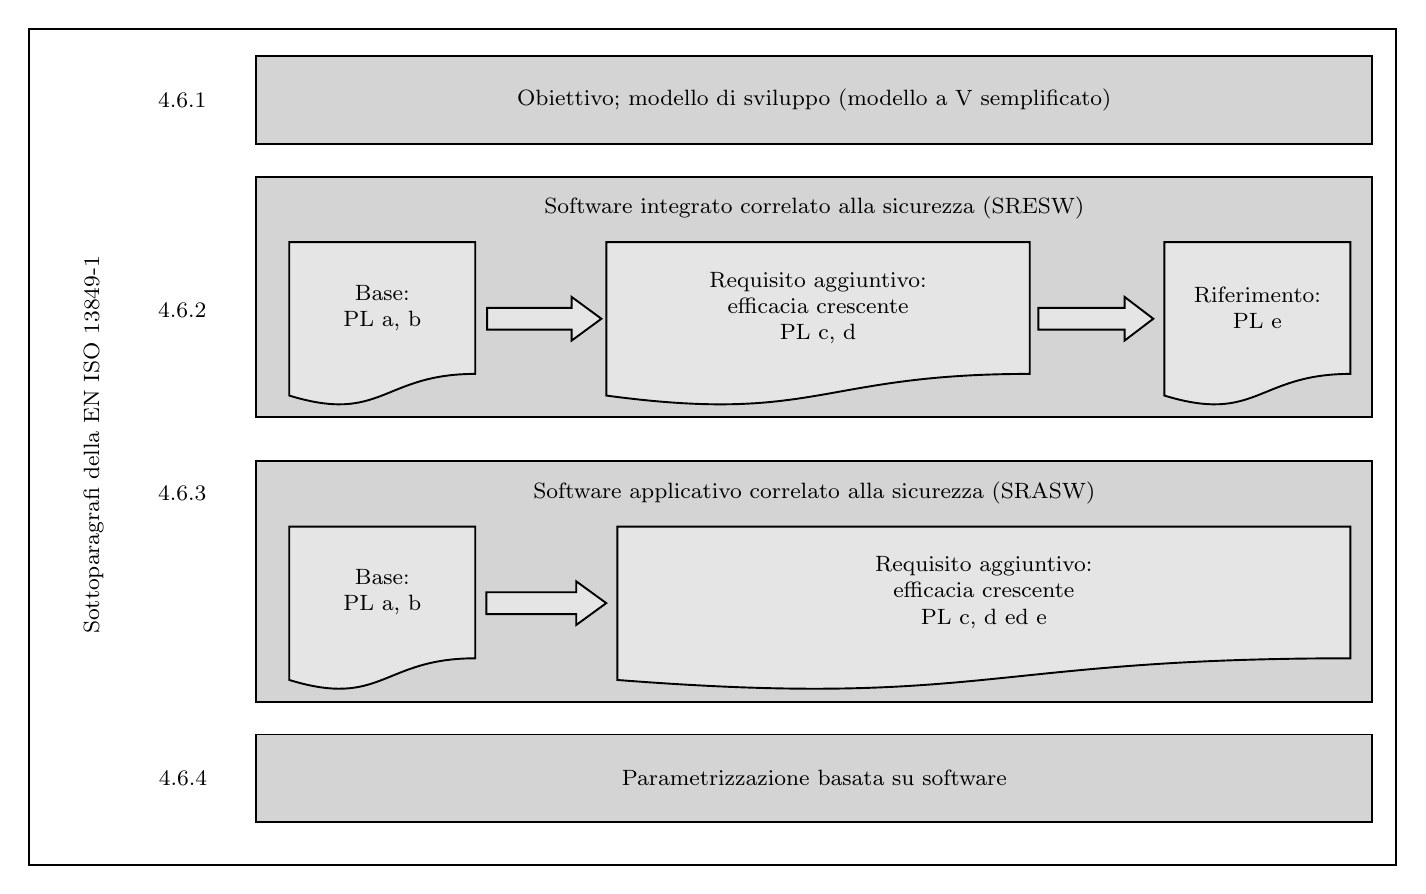
\begin{tikzpicture}[
  x=0.042cm, y=0.042cm,
  font=\footnotesize,
  cornice/.style={draw=black, line width=0.9pt},
  fascia/.style={draw=black, fill=black!17, line width=0.69pt},
  strappato/.style={draw=black, fill=black!10, line width=0.69pt},
  frecciona/.style={draw=black, fill=black!10, line width=0.69pt}
]

\setstretch{1}

% --- 4.6.1 ----------------------------------------------------------------
\draw[fascia] (69.10,218.40) rectangle (406.53,244.87);
\node at (46.76,231.64) {4.6.1};
\node at (237.82,231.64) {Obiettivo; modello di sviluppo (modello a V semplificato)};

% --- 4.6.2: software integrato (SRESW) ------------------------------------
\draw[fascia] (69.10,135.70) rectangle (406.53,208.48);
\node at (46.76,167.95) {4.6.2};
\node at (237.82,198.85) {Software integrato correlato alla sicurezza (SRESW)};

\draw[strappato] (79.09,188.65) -- (135.32,188.65) -- (135.32,148.82)
  .. controls (107.20,148.82) and (107.20,133.65) .. (79.09,142.27) -- cycle;
\node[align=center] at (107.21,168.70) {Base:\\PL a, b};

\draw[strappato] (174.96,188.65) -- (302.97,188.65) -- (302.97,148.82)
  .. controls (238.97,148.82) and (238.97,133.65) .. (174.96,142.27) -- cycle;
\node[align=center] at (238.97,168.70)
  {Requisito aggiuntivo:\\efficacia crescente\\PL c, d};

\draw[strappato] (343.67,188.65) -- (399.90,188.65) -- (399.90,148.82)
  .. controls (371.79,148.82) and (371.79,133.65) .. (343.67,142.27) -- cycle;
\node[align=center] at (371.79,168.70) {Riferimento:\\PL e};

\draw[frecciona] (138.92,168.79) -- (164.46,168.79) -- (164.46,172.09) --
  (173.46,165.49) -- (164.46,158.89) -- (164.46,162.19) -- (138.92,162.19) -- cycle;
\draw[frecciona] (305.58,168.79) -- (331.63,168.79) -- (331.63,172.09) --
  (340.31,165.49) -- (331.63,158.89) -- (331.63,162.19) -- (305.58,162.19) -- cycle;

% --- 4.6.3: software applicativo (SRASW) ----------------------------------
\draw[fascia] (69.10,49.72) rectangle (406.53,122.50);
\node at (46.76,112.75) {4.6.3};
\node at (237.82,112.75) {Software applicativo correlato alla sicurezza (SRASW)};

\draw[strappato] (79.09,102.67) -- (135.32,102.67) -- (135.32,62.84)
  .. controls (107.20,62.84) and (107.20,47.67) .. (79.09,56.29) -- cycle;
\node[align=center] at (107.21,82.76) {Base:\\PL a, b};

\draw[strappato] (178.27,102.67) -- (399.90,102.67) -- (399.90,62.84)
  .. controls (289.08,62.84) and (289.08,47.67) .. (178.27,56.29) -- cycle;
\node[align=center] at (289.08,82.76)
  {Requisito aggiuntivo:\\efficacia crescente\\PL c, d ed e};

\draw[frecciona] (138.67,82.81) -- (165.85,82.81) -- (165.85,86.11) --
  (174.92,79.52) -- (165.85,72.91) -- (165.85,76.21) -- (138.67,76.21) -- cycle;

% --- 4.6.4 ----------------------------------------------------------------
\draw[fascia] (69.10,13.33) rectangle (406.53,39.80);
\node at (46.96,26.57) {4.6.4};
\node at (237.82,26.57) {Parametrizzazione basata su software};

% --- dicitura verticale a sinistra ----------------------------------------
\node[rotate=90] at (19.96,127.35) {Sottoparagrafi della EN ISO 13849-1};

% --- cornice esterna --------------------------------------------------------
\draw[cornice] (0.38,0.37) rectangle (413.73,253.12);

\end{tikzpicture}
}
        \captionof{figure}{Graduazione dei requisiti per il software correlato alla sicurezza (EN~ISO~13849-1).}
        \label{fig:06-12}
    \end{minipage}
\end{center}

L'aspetto della “efficacia maggiore” si riferisce al livello crescente di prevenzione dei guasti. Ciò può essere illustrato mediante l'importante compito della produzione della specifica. Per il PL c, ad esempio, può essere sufficiente che i programmatori redigano essi stessi la specifica e che questa venga riesaminata da altri (riesame interno). Qualora lo stesso software venga tuttavia impiegato per il PL e, deve essere raggiunto un livello più elevato di prevenzione dei guasti. Potrebbe quindi essere necessario che la specifica venga redatta, ad esempio, dal responsabile del progetto software anziché dai programmatori. Inoltre, il riesame di tale specifica potrebbe essere effettuato congiuntamente a una persona più indipendente, come il responsabile dell'ingegnerizzazione hardware. Più occhi (in generale) individuano più errori. Una trattazione esaustiva dei singoli requisiti e della loro efficacia maggiore o minore esula purtroppo dall'ambito del presente rapporto. La trattazione sarà pertanto limitata a determinati casi particolari:
\begin{itemize}
    \item non è raro che il software coeso di un SRP/CS implementi diverse funzioni di sicurezza (SFx) con PL\textsubscript{r} differenti (ad es. SF1 e SF2 con PL\textsubscript{r} c, SF3 con PL\textsubscript{r} e). Nella pratica, tuttavia, è improbabile poter differenziare tra le funzioni di sicurezza con PL\textsubscript{r} differenti nel ciclo di sviluppo, negli strumenti o nell'efficacia delle attività (ad esempio durante le modifiche). In questo caso, i requisiti per la prevenzione dei guasti sono pertanto orientati al PL\textsubscript{r} più elevato (nell'esempio riportato: e).
    \item SRP/CS ridondanti di cui un solo canale è programmabile: sebbene l'elettronica programmabile costituisca un unico canale, la struttura complessiva soddisfa la Categoria 3 o 4. Funzioni di sicurezza con un PL\textsubscript{r} più elevato, quali d o e, vengono frequentemente implementate mediante tali strutture. Se l'elettronica programmabile viene impiegata in un canale della parte del sistema di comando in ridondanza diversificata con una tecnologia diversa dall'elettronica programmabile (ad es. tecnologia fluidica) nell'altro canale, la raccomandazione dell'IFA è che i requisiti normativi possano essere ridotti di un livello di PL, ad esempio per un PL\textsubscript{r} c anziché un PL\textsubscript{r} d, a causa della minore probabilità di un guasto pericoloso causato da guasti sistematici in questo SRASW. Indipendentemente da ciò, devono comunque essere osservati i requisiti normativi per l'SRESW (sottoparagrafo 6.3.10).
    \item impiego di PLC standard: gli esempi di circuiti riportati nel presente rapporto (cfr. Capitolo 8, pag. 99 e segg.) dimostrano che i PLC standard possono in linea di principio essere impiegati anche per l'ingegnerizzazione di sistemi di comando correlati alla sicurezza. Solo per il PL e risulta probabilmente molto difficile raggiungere il livello "alto" richiesto di copertura diagnostica DC pari almeno al 99\% per l'hardware di un PLC — quantomeno se tale copertura diagnostica deve essere implementata mediante l'SRASW. Per i PL da a a d, i requisiti software per il PLC standard sono descritti nel sottoparagrafo 6.3.10. Anche durante la programmazione applicativa devono essere soddisfatti i requisiti per la prevenzione degli errori nell'SRASW (sottoparagrafi 4.6.1 e 4.6.3 della norma) in conformità al PL\textsubscript{r}. L'argomento della capacità sistematica richiede particolare attenzione.
    \item un vantaggio nello sviluppo di SRESW diversificato consiste nel fatto che, su SRP/CS a due canali per una o più funzioni di sicurezza con un PL\textsubscript{r} pari a e, l'SRESW dei due canali può essere implementato in modo diversificato. Qualora il grado di tale diversità sia talmente elevato che il codice, la progettazione e persino la specifica siano stati creati in modo differente, questo software può anche essere sviluppato in conformità ai requisiti stabiliti dalla EN ISO 13849-1 per il PL d. È allora irrilevante se gli SRP/CS dispongano di due canali hardware diversi o identici.
\end{itemize}

\subsection{Strumenti software idonei}
\label{subsec:06-3-7}
Nessun software senza strumenti: questo vale in particolare per il software correlato alla sicurezza. La selezione e la qualità di tali strumenti costituiscono pertanto fattori determinanti per la prevenzione degli errori e quindi per la qualità della funzione di sicurezza. La EN ISO 13849-1 pone l'accento su quattro elementi:
\begin{itemize}
    \item \textit{strumenti di sviluppo}: lo sviluppo richiede strumenti idonei e collaudati per l'uso previsto. Per l'SRASW vengono generalmente impiegati strumenti certificati per componenti di sicurezza. Funzionalità quali la prevenzione e la rilevazione di errori semantici, il rispetto di sottoinsiemi del linguaggio o il monitoraggio delle linee guida di programmazione sollevano i programmatori da determinati compiti e migliorano la qualità del software.
    \item \textit{librerie di funzioni software}: la progettazione del sistema dovrebbe tenere conto delle librerie esistenti o fornite e, ove praticabile, impiegare funzioni validate. Si applica il seguente principio: quanto più il programma si basa su funzioni già validate o addirittura certificate, tanto minori saranno i componenti software specifici del progetto che devono essere validati internamente o da un organismo esterno prima della messa in servizio. Per le funzioni tipiche ricorrenti, agli integratori di sistema conviene investire l'impegno necessario nello sviluppare autonomamente moduli idonei conformi alla EN ISO 13849-1, in modo tale che possano anche essere riutilizzati e testati, anche da persone indipendenti, in modo routinario ed esente da errori. Anche le singole funzioni di libreria richiedono specifica, progettazione, piano di test, validazione, ecc.
    \item \textit{linguaggi di programmazione idonei}: per l'SRASW si raccomandano linguaggi orientati all'applicazione, ad esempio conformi alla IEC 61131-3 [46]. Anche tali linguaggi risultano più ampi del necessario e contengono costrutti che in alcuni casi sono soggetti a errori. I programmatori dovrebbero pertanto limitare l'uso della sintassi. I corrispondenti sottoinsiemi del linguaggio sono generalmente specificati dallo strumento stesso.
    \item \textit{linee guida di programmazione}: per la codifica delle funzioni software devono essere osservate linee guida di programmazione idonee [47]. Le linee guida dovrebbero essere le regole esistenti e riconosciute di un'organizzazione accreditata. In alternativa, un'azienda può elaborare proprie linee guida di programmazione idonee, purché queste abbiano un solido fondamento pratico o teorico. Le linee guida di programmazione disciplinano l'uso di costrutti linguistici critici, l'ambito e l'interfaccia delle funzioni software, la formattazione e i commenti del codice, i nomi simbolici di funzioni e variabili, ecc.
\end{itemize}

Tali strumenti e linee guida dovrebbero essere specificati nel documento di progettazione.

\subsection{Poco amate, ma importanti: la documentazione e la gestione della configurazione}
\label{subsec:06-3-8}
Prima che il fabbricante rilasci la dichiarazione CE di conformità per una macchina, deve redigere la relativa documentazione tecnica. Per quanto riguarda il software legato alla sicurezza, ciò si riferisce anzitutto alla specifica delle funzioni di sicurezza realizzate (specifica dei requisiti), al documento di progettazione (specifica tecnica) e al programma adeguatamente commentato. Devono inoltre essere elencate le funzioni di libreria certificate o auto validate utilizzate, unitamente alla loro identificazione (numero di versione, autore, data, ecc.). Deve inoltre essere documentata l'applicazione delle linee guida di programmazione proprie del fabbricante e dei sottoinsiemi linguistici (Language subsets) impiegati. Qualora queste siano già contenute nello strumento di sviluppo, è sufficiente un riferimento appropriato a tali proprietà. Infine, devono essere documentate le attività di test. Il test di integrazione e la validazione delle funzioni di sicurezza sono spesso eseguiti contestualmente. Questi test devono ovviamente essere pianificati e devono essere documentati insieme ai relativi risultati.

Che cosa si intende per gestione della configurazione? In particolare, per il software legato alla sicurezza, è evidente – e quindi costituisce un requisito – che il suo sviluppo sia trasparente per tutte le parti coinvolte e per successive verifiche ispettive:
\begin{itemize}
    \item chi ha eseguito la specifica, la programmazione, la messa in servizio, la verifica e la validazione, e quando?
    \item che cosa è stato utilizzato per lo sviluppo, ad esempio gli strumenti e le relative impostazioni, le funzioni riutilizzate e la loro identificazione, le linee guida di programmazione?
    \item quali versioni del programma sono caricate su quali SRP/CS?
\end{itemize}

Queste e altre informazioni necessarie, compresi tutti i documenti di sviluppo pertinenti, devono essere registrate e adeguatamente archiviate per un utilizzo successivo, ad esempio in caso di modifica dopo diversi anni di funzionamento.

\subsection{Il software è in costante evoluzione: modifica}
\label{subsec:06-3-9}
L'esperienza ha dimostrato che, anche dopo essere stato inizialmente testato, il SRASW è ancora oggetto di intensi lavori di estensione e adattamento durante la messa in servizio di un impianto o di una macchina. Questa procedura viene definita "modifica". Tali modifiche sono spesso così estese che non solo il codice, ma persino la specifica originaria non è più adeguata e dovrebbe essere effettivamente rivista. Le modifiche alle funzioni di sicurezza a un'estremità dell'impianto o della macchina possono avere un impatto anche sulle funzioni di sicurezza all'altra estremità che, in questa fase, non sono state modificate. Allo stesso modo, le modifiche possono rivelare lacune nel concetto di sicurezza. Questa possibilità deve essere esaminata, ripetendo se del caso le fasi necessarie del modello a V.

L'esperienza pratica mostra tuttavia che, anche dopo l'installazione, una macchina o un impianto può richiedere, ad esempio, un ulteriore dispositivo di arresto di emergenza o un riparo mobile aggiuntivo. Anche il processo di lavorazione viene spesso migliorato: anche in questo caso il concetto di sicurezza deve essere adattato. Il software esistente deve essere "modificato". Nota: ciò può verificarsi su SRP/CS già in funzione da un periodo di tempo prolungato e per lo più senza guasti causati da difetti del software - il che potrebbe però anche significare semplicemente che un guasto presente ma "nascosto" non si è ancora manifestato. A seguito di una modifica, tuttavia, questa situazione può cambiare, ad esempio se il software non era stato strutturato adeguatamente e i singoli moduli/funzioni non sono pertanto del tutto privi di influenza reciproca.

Nelle situazioni descritte, si manifesta spesso la "legge di Murphy": il programma è stato scritto molti anni prima, ma i programmatori originari hanno ora compiti più urgenti o hanno già lasciato l'azienda. In questo caso, è nell'interesse sia della sicurezza sia dell'economia della macchina o dell'impianto che il software possieda le proprietà sopra indicate: leggibilità, struttura, comprensibilità, e anche la possibilità di una modifica semplice e poco soggetta a errori - indipendentemente dal personale di programmazione di volta in volta disponibile.

In linea di principio, una modifica comporta che il processo di progettazione debba essere riavviato, ossia, nel modello a V, dal punto in cui è stata apportata una modifica (Figura 6.11), ad esempio:
\begin{itemize}
    \item quando il codice è stato modificato, devono essere ripetuti il test di modulo e il test di integrazione, così come la validazione;
    \item se sono state necessarie modifiche anche alla specifica, anch'essa deve essere nuovamente verificata, ad esempio mediante revisione da parte di un collega, al fine di garantire che non si siano insinuati guasti in un altro punto della specifica. Di conseguenza, devono essere ripetute tutte le misure di sviluppo e verifica, nonché la validazione delle funzioni di sicurezza interessate;
\end{itemize}

Alla luce dell'impegno descritto, è comprensibile che l'influenza di una modifica sulle funzioni di sicurezza debba essere studiata e documentata in modo sistematico. Poiché le modifiche possono avere un effetto non trascurabile sulla corretta esecuzione della funzione di sicurezza, occorre stabilire fin dall'inizio una procedura idonea. Se del caso, questa dovrebbe comprendere anche la nomina dei responsabili.

\subsection{Requisiti per il software dei componenti standard nelle SRP/CS}
\label{subsec:06-3-10}
I comandi legati alla sicurezza sono spesso realizzati mediante componenti standard per applicazioni industriali. Poiché la norma formula requisiti per la realizzazione del SRESW e del SRASW, questi devono essere soddisfatti anche per quanto riguarda i componenti standard elettronicamente programmabili. Esistono tuttavia restrizioni che non si applicano ai componenti di sicurezza collaudati.

\textit{Requisiti per il SRESW}
L'impiego di componenti standard industriali di provenienza esterna, non sviluppati specificamente per l'uso in funzioni di sicurezza e contenenti software embedded, non era in precedenza trattato dalla EN ISO 13849-1. Esistono tuttavia in pratica numerosi esempi di SRP/CS che fanno uso di componenti standard quali PLC, convertitori di frequenza o sensori, e che realizzano la sicurezza, ad esempio, mediante ridondanza diversificata con rilevamento dei guasti a livello di sistema. Un esempio che impiega un PLC standard e un convertitore di frequenza standard è mostrato nell'Allegato I della norma. Poiché l'osservanza dei requisiti SRESW non è generalmente confermata dal fabbricante per tali componenti standard e non può essere eseguita successivamente dall'integratore, in passato la soddisfazione dei requisiti SRESW non veniva dimostrata.
La EN ISO 13849-1, al punto 4.6.2, ora dispensa dalla necessità di dimostrare la soddisfazione dei requisiti SRESW per tali componenti standard, a condizione che siano soddisfatte le seguenti condizioni:
\begin{itemize}
    \item la SRP/CS è limitata a PL a o PL b e utilizza le categorie B, 2 o 3;
    \item la SRP/CS è limitata a PL c o PL d ed è ammesso l'impiego di più componenti per due canali nelle categorie 2 o 3. I componenti in questi due canali impiegano tecnologie diverse. Il requisito di tecnologie diverse nei due canali comporta una forte riduzione della probabilità che un guasto pericoloso della SRP/CS sia causato da un errore nel SRESW.
\end{itemize}

Oltre ai requisiti SRESW, la norma stabilisce ulteriori requisiti, riguardanti più propriamente l'hardware, che devono essere soddisfatti quando componenti standard sono utilizzati per la SRP/CS. Questi comprendono l'evitamento e il controllo dei guasti sistematici, nonché l'idoneità alle condizioni ambientali previste, quali clima, vibrazioni e compatibilità elettromagnetica (CEM). Questi requisiti aggiuntivi continuano ad applicarsi indipendentemente dal SRESW. Essi comprendono inoltre il requisito di applicare i principi di sicurezza di base a partire dalla categoria B in su, e i principi di sicurezza ben collaudati a partire dalla categoria 1 in su. Devono inoltre essere soddisfatti, per tutte le categorie, i requisiti di base della categoria B, ossia: la SRP/CS deve essere progettata, costruita, selezionata, assemblata e combinata almeno in conformità alle norme pertinenti, ad esempio la IEC 61131-2 per i PLC e la IEC 61800-1/2 per i convertitori di frequenza.

Lo sviluppo con assicurazione della qualità secondo la serie ISO 900x non è reso un requisito esplicito dalla norma; esso può tuttavia essere considerato un principio di sicurezza di base per quanto riguarda l'impiego di componenti standard.
La Tabella~\ref{tab:06-6} mostra le combinazioni possibili di PL e categoria con componenti standard, e se e in che modo i requisiti relativi al SRESW debbano essere soddisfatti.

Resta da chiarire che cosa si intenda per "diversità tecnologica". Con questo termine si intende che, grazie alla diversità tra due canali (la differenza tra le tecnologie impiegate), la probabilità che un guasto pericoloso della SRP/CS sia causato da un errore nel SRESW risulta fortemente ridotta. In questo contesto sono rilevanti i guasti sistematici e i guasti per causa comune.

% Tabella non fluttuante (minipage + \captionof): a fine capitolo un float
% finirebbe da solo su una pagina a parte.
% \setstretch{1} e' necessario perche' \onehalfspacing e' globale e qui
% quasi tutte le celle vanno a capo su piu' righe.
\begin{center}
    \begin{minipage}{\textwidth}
    \captionsetup{hypcap=false}
    \definecolor{tabblue}{RGB}{31,73,125}
    \setlength{\tabcolsep}{3pt}
    \renewcommand{\arraystretch}{1.2}
    \setstretch{1}
    \small
    \captionof{table}{Requisiti per il SRESW dei componenti standard (secondo la EN~ISO~13849-1).}
    \label{tab:06-6}
    \begin{tabularx}{\textwidth}{%
        |>{\raggedright\arraybackslash}p{2.7cm}%
        |>{\raggedright\arraybackslash}p{1.3cm}%
        |>{\raggedright\arraybackslash}p{1.7cm}%
        |>{\raggedright\arraybackslash}p{5.3cm}%
        |>{\raggedright\arraybackslash}X|}
        \hline
        \rowcolor{tabblue}
        \textcolor{white}{\textbf{Combinazione n.}} &
        \multicolumn{1}{c|}{\textcolor{white}{\textbf{PL}}} &
        \textcolor{white}{\textbf{Categoria}} &
        \multicolumn{1}{c|}{\textcolor{white}{\textbf{Condizioni}}} &
        {\centering\textcolor{white}{\textbf{Requisiti per il SRESW dei componenti standard}}\par} \\
        \hline
        \rowcolor{black!8}
        1 & a, b & B, 2, 3 &
        \begin{itemize}[label=\textbullet, leftmargin=1em, nosep, topsep=2pt]
            \item Conformità alle norme di prodotto pertinenti
            \item Progettazione con assicurazione della qualità come principio di sicurezza di base
        \end{itemize} &
        Ai componenti standard industriali non si applicano requisiti relativi al SRESW\@. \\
        \hline
        2 & a, b, c & 1 &
        La realizzazione mediante componenti elettronici non è generalmente possibile, poiché essi non sono considerati componenti collaudati ai sensi del sottoparagrafo 6.2.4 della EN~ISO~13849-1 &
        \\
        \hline
        \rowcolor{black!8}
        3 & c, d & 2, 3 &
        \begin{itemize}[label=\textbullet, leftmargin=1em, nosep, topsep=2pt]
            \item Come al n.~1
            \item Due canali con diversità tecnologica; la rilevazione dei guasti richiesta (\textit{DC}) è realizzata mediante SRASW
        \end{itemize} &
        Ai componenti standard industriali non si applicano requisiti relativi al SRESW\@. \\
        \hline
        4 & c, d & 2, 3 &
        Due canali senza diversità tecnologica; la rilevazione dei guasti richiesta (\textit{DC}) è realizzata mediante SRASW &
        Si applicano integralmente i requisiti relativi al SRESW conformemente al sottoparagrafo 4.6.2 della EN~ISO~13849-1, anche ai componenti standard industriali. È richiesta un'analisi di sicurezza da parte del fabbricante del componente. \\
        \hline
        \rowcolor{black!8}
        5 & e & 3, 4 &
        Il sottoparagrafo 4.6.2 della norma stabilisce che il PL~e non è possibile con componenti standard. &
        \\
        \hline
    \end{tabularx}
    \end{minipage}
\end{center}

Il requisito di "diversità tecnologica" può normalmente essere considerato soddisfatto negli esempi seguenti:
\begin{itemize}
    \item un canale (canale funzionale o canale di test) impiega componenti contenenti software embedded. Il secondo canale impiega esclusivamente componenti privi di software embedded, ossia componenti meccanici, elettronici, elettromeccanici, pneumatici o idraulici.
    \item  due canali impiegano software embedded diversificato, ad esempio sistemi operativi differenti eseguiti su hardware identico o differente.\\
    Nota: quando viene utilizzato hardware identico, occorre prestare particolare attenzione alla capacità sistematica dei componenti in relazione al Performance Level richiesto.
    \item i due canali impiegano hardware differente (ad es. microprocessori con core diversi), poiché si presume che il relativo software embedded sia stato programmato in ambienti di sviluppo differenti.
\end{itemize}

Il requisito di "diversità tecnologica" può normalmente essere considerato non soddisfatto negli esempi seguenti:
\begin{itemize}
    \item i due canali impiegano componenti dello stesso tipo di fabbricanti diversi, senza ulteriori informazioni sulla diversità del software embedded. In questo scenario, non può generalmente essere escluso che i due fabbricanti utilizzino gli stessi componenti software embedded, ed eventualmente persino hardware identico (con marchiatura del marchio);
    \item i due canali impiegano componenti di tipo diverso dello stesso fabbricante, senza ulteriori informazioni sul software embedded.
\end{itemize}

\section{Combinazione di SRP/CS come sottosistemi}
\label{sec:06-4}
Fino a questo punto, il presente capitolo ha considerato una SRP/CS soltanto nella forma di un sistema di comando completo, integralmente riconducibile a una categoria o a un'architettura designata con il corrispondente Performance Level. La funzione di sicurezza viene eseguita interamente da un tale sistema di comando, a partire da un evento iniziatore fino al raggiungimento dello stato sicuro. Nella realtà, tuttavia, è spesso necessario che più SRP/CS, ciascuna delle quali esegue parti della funzione di sicurezza, siano disposte in serie come sottosistemi. Tali sottosistemi possono impiegare tecnologie diverse e/o realizzare categorie o Performance Level differenti. Frequentemente, ad esempio, vengono impiegate tecnologie diverse a livello di sensore/logica (es. elettronica in categoria 3) rispetto al livello di azionamento (es. idraulica in categoria 1), oppure vengono interconnessi dispositivi acquistati esternamente, ad esempio barriere fotoelettriche, comandi elettronici e livello di valvole pneumatiche, come mostrato nella Figura~\ref{fig:06-13}.

% La minipage tiene insieme disegno e didascalia (figura non fluttuante)
\begin{center}
    \begin{minipage}{\textwidth}
        \centering
        \captionsetup{hypcap=false}
        \resizebox{0.9\textwidth}{!}{%==============================================================
%  Figura 6.13 - Disposizione in serie di sottosistemi per la
%  realizzazione di una funzione di sicurezza
%  Adattamento in italiano della Figura 6.13 dell'IFA Report 2/2017
%
%  A differenza delle altre figure del capitolo, qui il disegno non e'
%  stato ricostruito a mano: i simboli (cilindro, barriera, valvola,
%  schemi a blocchi) sono troppi e troppo minuti. Il blocco "geometria"
%  qui sotto e' la conversione automatica dei 249 tracciati vettoriali
%  della pagina 72 di rep0217e.pdf, che non contengono testo; le
%  diciture italiane sono poi collocate a mano in fondo al file, sulle
%  posizioni misurate nell'originale.
%  Per rigenerare la geometria occorre riconvertire la pagina: il
%  blocco non va modificato a mano.
%
%  Sistema di riferimento: l'origine e' l'angolo in basso a sinistra
%  della cornice; l'asse y e' rivolto verso l'alto; una unita' e' un
%  punto PostScript del disegno originale.
%==============================================================
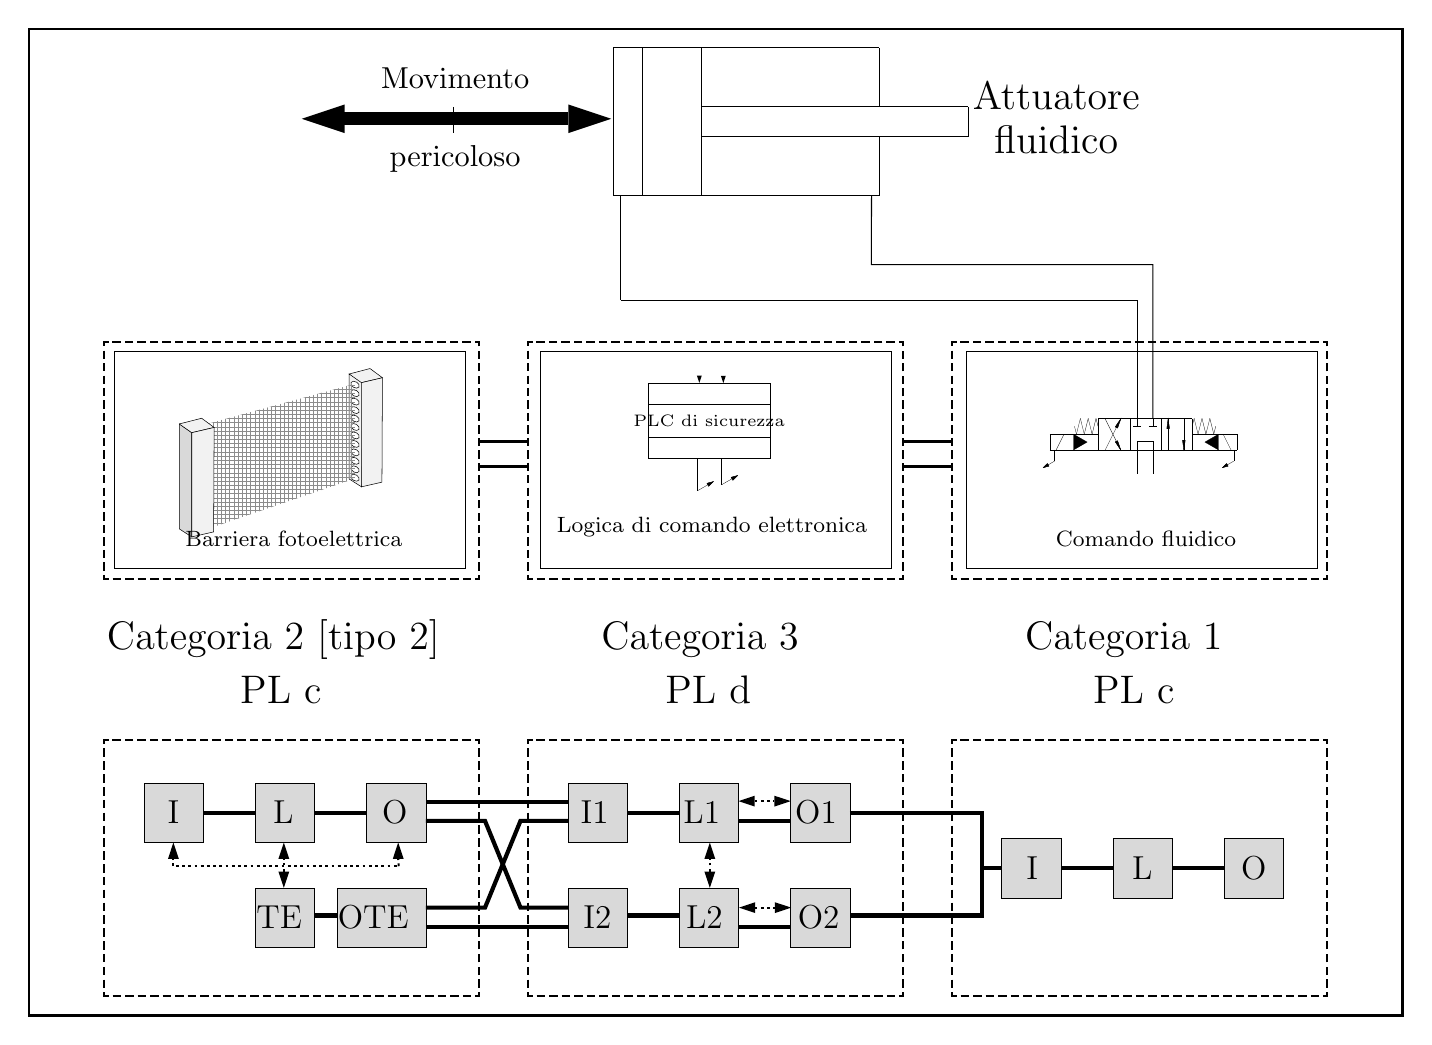
\begin{tikzpicture}[
  x=0.035cm, y=0.035cm,
  piccolo/.style={font=\fontsize{8.2}{9.5}\selectfont},
  medio/.style={font=\fontsize{11}{13}\selectfont},
  grande/.style={font=\fontsize{13.7}{16}\selectfont},
  siglablocco/.style={font=\fontsize{12.6}{15}\selectfont}
]

\setstretch{1}

% ============ geometria (conversione automatica, non modificare) ============
\filldraw[fill=white, draw=black, line width=0.19pt] (340.02,240.97) -- (467.39,240.97) -- (467.39,162.26) -- (340.02,162.26) -- cycle;
\filldraw[fill=white, draw=black, line width=0.19pt] (185.46,240.97) -- (312.83,240.97) -- (312.83,162.26) -- (185.46,162.26) -- cycle;
\filldraw[fill=white, draw=black, line width=0.19pt] (30.91,240.97) -- (158.27,240.97) -- (158.27,162.26) -- (30.91,162.26) -- cycle;
\fill[fill=black] (114.49,320.22) -- (98.95,325.4) -- (114.49,330.58) -- cycle;
\fill[fill=black] (195.68,330.58) -- (211.22,325.4) -- (195.68,320.22) -- cycle;
\draw[draw=black, line width=0.75pt] (335.01,159.95) -- (335.01,158.44) -- (336.53,158.44);
\draw[draw=black, line width=0.75pt, dash pattern=on 3.01pt off 1.51pt] (338.03,158.44) -- (468.69,158.44);
\draw[draw=black, line width=0.75pt] (469.45,158.44) -- (470.96,158.44) -- (470.96,159.95);
\draw[draw=black, line width=0.75pt, dash pattern=on 3.00pt off 1.50pt] (470.96,161.46) -- (470.96,242.04);
\draw[draw=black, line width=0.75pt] (470.96,242.79) -- (470.96,244.31) -- (469.45,244.31);
\draw[draw=black, line width=0.75pt, dash pattern=on 3.01pt off 1.51pt] (467.94,244.31) -- (337.28,244.31);
\draw[draw=black, line width=0.75pt] (336.53,244.31) -- (335.01,244.31) -- (335.01,242.79);
\draw[draw=black, line width=0.75pt, dash pattern=on 3.00pt off 1.50pt] (335.01,241.29) -- (335.01,160.71);
\draw[draw=black, line width=0.75pt] (181.17,159.95) -- (181.17,158.44) -- (182.68,158.44);
\draw[draw=black, line width=0.75pt, dash pattern=on 3.01pt off 1.51pt] (184.19,158.44) -- (314.85,158.44);
\draw[draw=black, line width=0.75pt] (315.6,158.44) -- (317.12,158.44) -- (317.12,159.95);
\draw[draw=black, line width=0.75pt, dash pattern=on 3.00pt off 1.50pt] (317.12,161.46) -- (317.12,242.04);
\draw[draw=black, line width=0.75pt] (317.12,242.79) -- (317.12,244.31) -- (315.61,244.31);
\draw[draw=black, line width=0.75pt, dash pattern=on 3.01pt off 1.51pt] (314.1,244.31) -- (183.44,244.31);
\draw[draw=black, line width=0.75pt] (182.69,244.31) -- (181.17,244.31) -- (181.17,242.79);
\draw[draw=black, line width=0.75pt, dash pattern=on 3.00pt off 1.50pt] (181.17,241.29) -- (181.17,160.71);
\draw[draw=black, line width=0.75pt] (27.33,159.95) -- (27.33,158.44) -- (28.84,158.44);
\draw[draw=black, line width=0.75pt, dash pattern=on 3.01pt off 1.51pt] (30.35,158.44) -- (161.01,158.44);
\draw[draw=black, line width=0.75pt] (161.76,158.44) -- (163.28,158.44) -- (163.28,159.95);
\draw[draw=black, line width=0.75pt, dash pattern=on 3.00pt off 1.50pt] (163.28,161.46) -- (163.28,242.04);
\draw[draw=black, line width=0.75pt] (163.28,242.79) -- (163.28,244.31) -- (161.77,244.31);
\draw[draw=black, line width=0.75pt, dash pattern=on 3.01pt off 1.51pt] (160.26,244.31) -- (29.6,244.31);
\draw[draw=black, line width=0.75pt] (28.85,244.31) -- (27.33,244.31) -- (27.33,242.79);
\draw[draw=black, line width=0.75pt, dash pattern=on 3.00pt off 1.50pt] (27.33,241.29) -- (27.33,160.71);
\draw[draw=black, line width=1.13pt] (316.83,208.41) -- (334.73,208.41);
\draw[draw=black, line width=1.13pt] (317.12,199.11) -- (335.01,199.11);
\draw[draw=black, line width=1.13pt] (162.99,208.41) -- (180.89,208.41);
\draw[draw=black, line width=1.13pt] (163.28,199.11) -- (181.17,199.11);
\draw[draw=black, line width=0.75pt] (27.33,8.5) -- (27.33,6.99) -- (28.84,6.99);
\draw[draw=black, line width=0.75pt, dash pattern=on 3.01pt off 1.51pt] (30.35,6.99) -- (161.01,6.99);
\draw[draw=black, line width=0.75pt] (161.76,6.99) -- (163.28,6.99) -- (163.28,8.5);
\draw[draw=black, line width=0.75pt, dash pattern=on 3.09pt off 1.55pt] (163.28,10.05) -- (163.28,97.72);
\draw[draw=black, line width=0.75pt] (163.28,98.49) -- (163.28,100.01) -- (161.77,100.01);
\draw[draw=black, line width=0.75pt, dash pattern=on 3.01pt off 1.51pt] (160.26,100.01) -- (29.6,100.01);
\draw[draw=black, line width=0.75pt] (28.85,100.01) -- (27.33,100.01) -- (27.33,98.49);
\draw[draw=black, line width=0.75pt, dash pattern=on 3.09pt off 1.55pt] (27.33,96.94) -- (27.33,9.28);
\filldraw[fill=black!15, draw=black, line width=0.19pt] (82.07,46.34) -- (103.53,46.34) -- (103.53,24.88) -- (82.07,24.88) -- cycle;
\draw[draw=black, line width=1.51pt] (63.11,73.53) -- (122.49,73.53);
\filldraw[fill=black!15, draw=black, line width=0.19pt] (41.64,84.26) -- (63.11,84.26) -- (63.11,62.8) -- (41.64,62.8) -- cycle;
\filldraw[fill=black!15, draw=black, line width=0.19pt] (82.07,84.26) -- (103.53,84.26) -- (103.53,62.8) -- (82.07,62.8) -- cycle;
\fill[fill=black!15] (122.5,84.26) -- (143.96,84.26) -- (143.96,62.8) -- (122.5,62.8) -- cycle;
\draw[draw=black, line width=0.19pt] (122.49,84.26) -- (143.96,84.26) -- (143.96,62.8) -- (122.49,62.8) -- cycle;
\fill[fill=black!15] (111.76,46.34) -- (143.96,46.34) -- (143.96,24.88) -- (111.76,24.88) -- cycle;
\draw[draw=black, line width=0.19pt] (111.76,46.34) -- (143.96,46.34) -- (143.96,24.88) -- (111.76,24.88) -- cycle;
\draw[draw=black, line width=0.75pt] (181.17,8.5) -- (181.17,6.99) -- (182.68,6.99);
\draw[draw=black, line width=0.75pt, dash pattern=on 3.01pt off 1.51pt] (184.19,6.99) -- (314.85,6.99);
\draw[draw=black, line width=0.75pt] (315.6,6.99) -- (317.12,6.99) -- (317.12,8.5);
\draw[draw=black, line width=0.75pt, dash pattern=on 3.09pt off 1.55pt] (317.12,10.05) -- (317.12,97.72);
\draw[draw=black, line width=0.75pt] (317.12,98.49) -- (317.12,100.01) -- (315.61,100.01);
\draw[draw=black, line width=0.75pt, dash pattern=on 3.01pt off 1.51pt] (314.1,100.01) -- (183.44,100.01);
\draw[draw=black, line width=0.75pt] (182.69,100.01) -- (181.17,100.01) -- (181.17,98.49);
\draw[draw=black, line width=0.75pt, dash pattern=on 3.09pt off 1.55pt] (181.17,96.94) -- (181.17,9.28);
\filldraw[fill=black!15, draw=black, line width=0.19pt] (195.48,84.26) -- (216.95,84.26) -- (216.95,62.8) -- (195.48,62.8) -- cycle;
\filldraw[fill=black!15, draw=black, line width=0.19pt] (235.91,84.26) -- (257.37,84.26) -- (257.37,62.8) -- (235.91,62.8) -- cycle;
\fill[fill=black!15] (276.33,84.26) -- (297.8,84.26) -- (297.8,62.8) -- (276.33,62.8) -- cycle;
\draw[draw=black, line width=0.19pt] (276.34,84.26) -- (297.8,84.26) -- (297.8,62.8) -- (276.34,62.8) -- cycle;
\draw[draw=black, line width=0.75pt] (335.01,8.5) -- (335.01,6.99) -- (336.53,6.99);
\draw[draw=black, line width=0.75pt, dash pattern=on 3.01pt off 1.51pt] (338.03,6.99) -- (468.69,6.99);
\draw[draw=black, line width=0.75pt] (469.45,6.99) -- (470.96,6.99) -- (470.96,8.5);
\draw[draw=black, line width=0.75pt, dash pattern=on 3.09pt off 1.55pt] (470.96,10.05) -- (470.96,97.72);
\draw[draw=black, line width=0.75pt] (470.96,98.49) -- (470.96,100.01) -- (469.45,100.01);
\draw[draw=black, line width=0.75pt, dash pattern=on 3.01pt off 1.51pt] (467.94,100.01) -- (337.28,100.01);
\draw[draw=black, line width=0.75pt] (336.53,100.01) -- (335.01,100.01) -- (335.01,98.49);
\draw[draw=black, line width=0.75pt, dash pattern=on 3.09pt off 1.55pt] (335.01,96.94) -- (335.01,9.28);
\draw[draw=black, line width=1.51pt] (345.39,53.5) -- (433.75,53.5);
\filldraw[fill=black!15, draw=black, line width=0.19pt] (352.9,64.23) -- (374.36,64.23) -- (374.36,42.76) -- (352.9,42.76) -- cycle;
\filldraw[fill=black!15, draw=black, line width=0.19pt] (393.33,64.23) -- (414.79,64.23) -- (414.79,42.76) -- (393.33,42.76) -- cycle;
\filldraw[fill=black!15, draw=black, line width=0.19pt] (433.75,64.23) -- (455.22,64.23) -- (455.22,42.76) -- (433.75,42.76) -- cycle;
\filldraw[fill=black!15, draw=black, line width=0.19pt] (195.48,46.34) -- (216.95,46.34) -- (216.95,24.88) -- (195.48,24.88) -- cycle;
\filldraw[fill=black!15, draw=black, line width=0.19pt] (235.91,46.34) -- (257.37,46.34) -- (257.37,24.88) -- (235.91,24.88) -- cycle;
\fill[fill=black!15] (276.33,46.34) -- (297.8,46.34) -- (297.8,24.88) -- (276.33,24.88) -- cycle;
\draw[draw=black, line width=0.19pt] (276.34,46.34) -- (297.8,46.34) -- (297.8,24.88) -- (276.34,24.88) -- cycle;
\draw[draw=black, line width=1.51pt] (103.53,36.32) -- (111.76,36.32);
\draw[draw=black, line width=1.51pt] (143.96,32.03) -- (195.48,32.03);
\draw[draw=black, line width=1.51pt] (143.96,39.19) -- (165.43,39.19) -- (178.31,70.67) -- (195.48,70.67);
\draw[draw=black, line width=1.51pt] (143.96,70.67) -- (165.43,70.67) -- (178.31,39.19) -- (195.48,39.19);
\draw[draw=black, line width=1.51pt] (143.96,77.4) -- (195.48,77.4);
\draw[draw=black, line width=1.51pt] (216.95,73.53) -- (235.91,73.53);
\draw[draw=black, line width=1.51pt] (216.95,36.32) -- (235.91,36.32);
\draw[draw=black, line width=1.51pt] (257.37,70.67) -- (276.34,70.67);
\fill[fill=black] (263.28,75.86) -- (257.38,77.83) -- (263.28,79.79) -- cycle;
\fill[fill=black] (270.43,79.79) -- (276.34,77.83) -- (270.43,75.85) -- cycle;
\draw[draw=black, line width=1.51pt] (257.55,32.03) -- (276.51,32.03);
\fill[fill=black] (263.46,37.22) -- (257.55,39.19) -- (263.46,41.15) -- cycle;
\fill[fill=black] (270.61,41.15) -- (276.51,39.19) -- (270.61,37.22) -- cycle;
\draw[draw=black, line width=1.51pt] (297.8,73.53) -- (345.74,73.53) -- (345.74,36.33) -- (297.8,36.33);
\fill[fill=black] (90.48,56.89) -- (92.44,62.8) -- (94.41,56.89) -- cycle;
\fill[fill=black] (94.41,52.25) -- (92.44,46.34) -- (90.48,52.25) -- cycle;
\fill[fill=black] (50.41,56.89) -- (52.37,62.8) -- (54.34,56.89) -- cycle;
\fill[fill=black] (131.98,56.89) -- (133.94,62.8) -- (135.91,56.89) -- cycle;
\fill[fill=black] (245.03,56.89) -- (247,62.8) -- (248.97,56.89) -- cycle;
\fill[fill=black] (248.97,52.25) -- (247,46.34) -- (245.03,52.25) -- cycle;
\draw[draw=black, line width=0.10pt] (402.03,196.6) -- (402.03,208.54);
\draw[draw=black, line width=0.10pt] (407.77,213.8) -- (407.77,216.65);
\draw[draw=black, line width=0.10pt] (400.62,213.78) -- (403.47,213.78);
\draw[draw=black, line width=0.10pt] (402.08,216.65) -- (402.08,213.8);
\draw[draw=black, line width=0.10pt] (407.77,196.6) -- (407.77,208.55);
\draw[draw=black, line width=0.10pt] (422.01,205.26) -- (410.62,205.26);
\draw[draw=black, line width=0.10pt] (422.01,216.65) -- (422.01,205.26);
\draw[draw=black, line width=0.10pt] (410.62,216.65) -- (422.01,216.65);
\draw[draw=black, line width=0.10pt] (399.23,216.65) -- (410.62,216.65);
\draw[draw=black, line width=0.10pt] (410.62,205.26) -- (399.23,205.26);
\draw[draw=black, line width=0.10pt] (387.84,205.26) -- (387.84,216.65);
\draw[draw=black, line width=0.10pt] (387.84,216.65) -- (399.23,216.65);
\draw[draw=black, line width=0.10pt] (399.23,205.26) -- (387.84,205.26);
\draw[draw=black, line width=0.10pt] (438.28,210.95) -- (422.01,210.95);
\draw[draw=black, line width=0.10pt] (438.28,205.26) -- (438.28,210.95);
\draw[draw=black, line width=0.10pt] (422.01,205.26) -- (438.28,205.26);
\draw[draw=black, line width=0.10pt] (370.42,210.94) -- (378.96,210.94);
\draw[draw=black, line width=0.10pt] (370.42,205.25) -- (370.42,210.94);
\draw[draw=black, line width=0.10pt] (433.25,210.95) -- (436.09,205.26);
\draw[draw=black, line width=0.10pt] (375.5,210.94) -- (372.65,205.25);
\draw[draw=black, line width=0.10pt] (410.62,205.26) -- (410.62,216.65);
\filldraw[fill=black, draw=black, line width=0.10pt] (431.55,210.94) -- (426.62,208.1) -- (431.55,205.25) -- cycle;
\filldraw[fill=black, draw=black, line width=0.10pt] (378.97,210.94) -- (383.9,208.1) -- (378.97,205.25) -- cycle;
\draw[draw=black, line width=0.10pt] (385.7,210.98) -- (387.12,216.68);
\draw[draw=black, line width=0.10pt] (381.43,216.68) -- (382.85,210.98);
\draw[draw=black, line width=0.10pt] (384.28,216.67) -- (382.85,210.98);
\draw[draw=black, line width=0.10pt] (381.43,216.67) -- (380.01,210.98);
\draw[draw=black, line width=0.10pt] (384.28,216.68) -- (385.7,210.98);
\draw[draw=black, line width=0.10pt] (380.01,210.98) -- (379.3,213.83);
\draw[draw=black, line width=0.10pt] (387.12,216.68) -- (387.84,213.83);
\draw[draw=black, line width=0.10pt] (426.99,210.98) -- (428.42,216.68);
\draw[draw=black, line width=0.10pt] (426.99,210.98) -- (425.57,216.68);
\draw[draw=black, line width=0.10pt] (428.42,216.68) -- (429.84,210.98);
\draw[draw=black, line width=0.10pt] (424.14,210.98) -- (422.72,216.68);
\draw[draw=black, line width=0.10pt] (424.14,210.98) -- (425.57,216.68);
\draw[draw=black, line width=0.10pt] (422.72,216.67) -- (422.01,213.83);
\draw[draw=black, line width=0.10pt] (429.84,210.98) -- (430.55,213.83);
\draw[draw=black, line width=0.10pt] (387.83,210.94) -- (371.56,210.94);
\draw[draw=black, line width=0.10pt] (387.84,205.25) -- (387.84,210.94);
\draw[draw=black, line width=0.10pt] (370.42,205.25) -- (387.84,205.25);
\draw[draw=black, line width=0.10pt] (268.95,229.57) -- (224.58,229.57) -- (224.58,222.04) -- (268.95,222.04) -- cycle;
\draw[draw=black, line width=0.10pt] (268.95,222.04) -- (224.58,222.04) -- (224.58,209.73) -- (268.95,209.73) -- cycle;
\draw[draw=black, line width=0.10pt] (251.23,202.3) -- (251.23,192.59);
\draw[draw=black, line width=0.10pt] (257.07,195.96) -- (251.23,192.59);
\filldraw[fill=black, draw=black, line width=0.10pt] (257.06,195.96) -- (254.73,195.33) -- (255.35,194.25) -- cycle;
\draw[draw=black, line width=0.10pt] (254.73,195.33) -- (257.07,195.96);
\draw[draw=black, line width=0.10pt] (255.35,194.25) -- (257.07,195.96);
\draw[draw=black, line width=0.10pt] (254.73,195.33) -- (255.35,194.25);
\draw[draw=black, line width=0.10pt] (242.47,202.3) -- (242.47,190.4);
\draw[draw=black, line width=0.10pt] (248.31,193.77) -- (242.47,190.4);
\filldraw[fill=black, draw=black, line width=0.10pt] (248.31,193.77) -- (245.97,193.15) -- (246.6,192.06) -- cycle;
\draw[draw=black, line width=0.10pt] (245.97,193.15) -- (248.31,193.77);
\draw[draw=black, line width=0.10pt] (246.6,192.06) -- (248.31,193.77);
\draw[draw=black, line width=0.10pt] (245.97,193.15) -- (246.6,192.06);
\draw[draw=black, line width=0.10pt] (224.58,209.91) -- (224.58,202.36) -- (268.95,202.36) -- (268.95,209.9);
\fill[fill=black] (252.79,232.14) -- (251.91,229.49) -- (251.03,232.14) -- cycle;
\fill[fill=black] (244.07,232.22) -- (243.18,229.58) -- (242.3,232.22) -- cycle;
\draw[draw=black, line width=0.10pt] (372.07,205.27) -- (372.07,201.18);
\draw[draw=black, line width=0.10pt] (367.99,198.83) -- (372.07,201.18);
\filldraw[fill=black, draw=black, line width=0.10pt] (367.99,198.83) -- (370.03,199.37) -- (369.49,200.32) -- cycle;
\draw[draw=black, line width=0.10pt] (370.03,199.37) -- (367.99,198.83);
\draw[draw=black, line width=0.10pt] (369.48,200.32) -- (367.99,198.83);
\draw[draw=black, line width=0.10pt] (370.03,199.37) -- (369.48,200.32);
\draw[draw=black, line width=0.10pt] (437.08,205.27) -- (437.08,201.18);
\draw[draw=black, line width=0.10pt] (433,198.83) -- (437.08,201.18);
\filldraw[fill=black, draw=black, line width=0.10pt] (433,198.83) -- (435.04,199.37) -- (434.49,200.32) -- cycle;
\draw[draw=black, line width=0.10pt] (435.04,199.37) -- (433,198.83);
\draw[draw=black, line width=0.10pt] (434.49,200.32) -- (433,198.83);
\draw[draw=black, line width=0.10pt] (435.04,199.37) -- (434.49,200.32);
\filldraw[fill=black!15, draw=black, line width=0.19pt] (59.03,173.7) -- (59.03,211.51) -- (54.52,214.68) -- (54.52,176.6) -- cycle;
\filldraw[fill=black!5, draw=black, line width=0.19pt] (128.22,231.44) -- (120.1,229.54) -- (116.13,232.79) -- (123.71,234.78) -- cycle;
\filldraw[fill=black!5, draw=black, line width=0.19pt] (128.22,231.44) -- (120.1,229.54) -- (120.63,191.87) -- (128.04,193.55) -- cycle;
\filldraw[fill=black!5, draw=black, line width=0.19pt] (120.63,191.87) -- (120.64,229.63) -- (116.13,232.8) -- (116.13,194.72) -- cycle;
\fill[fill=white] (118.82,229.85) .. controls (119.61,229.39) and (120.01,228.6) .. (119.71,228.08) .. controls (119.41,227.57) and (118.53,227.52) .. (117.73,227.97) .. controls (116.94,228.44) and (116.54,229.22) .. (116.84,229.74) .. controls (117.14,230.26) and (118.02,230.31) .. (118.82,229.85);
\draw[draw=black, line width=0.19pt] (118.82,229.85) .. controls (119.61,229.39) and (120.01,228.6) .. (119.71,228.08) .. controls (119.41,227.57) and (118.53,227.52) .. (117.73,227.97) .. controls (116.94,228.44) and (116.54,229.22) .. (116.84,229.74) .. controls (117.14,230.26) and (118.02,230.31) .. (118.82,229.85) -- cycle;
\fill[fill=white] (118.82,226.78) .. controls (119.61,226.32) and (120.01,225.53) .. (119.71,225.02) .. controls (119.41,224.5) and (118.53,224.45) .. (117.73,224.91) .. controls (116.94,225.36) and (116.54,226.16) .. (116.84,226.67) .. controls (117.14,227.19) and (118.02,227.24) .. (118.82,226.78);
\draw[draw=black, line width=0.19pt] (118.82,226.78) .. controls (119.61,226.32) and (120.01,225.53) .. (119.71,225.02) .. controls (119.41,224.5) and (118.53,224.45) .. (117.73,224.91) .. controls (116.94,225.36) and (116.54,226.16) .. (116.84,226.67) .. controls (117.14,227.19) and (118.02,227.24) .. (118.82,226.78) -- cycle;
\fill[fill=white] (118.82,223.71) .. controls (119.61,223.26) and (120.01,222.46) .. (119.71,221.95) .. controls (119.41,221.43) and (118.53,221.38) .. (117.73,221.84) .. controls (116.94,222.3) and (116.54,223.09) .. (116.84,223.6) .. controls (117.14,224.12) and (118.02,224.17) .. (118.82,223.71);
\draw[draw=black, line width=0.19pt] (118.82,223.71) .. controls (119.61,223.26) and (120.01,222.46) .. (119.71,221.95) .. controls (119.41,221.43) and (118.53,221.38) .. (117.73,221.84) .. controls (116.94,222.3) and (116.54,223.09) .. (116.84,223.6) .. controls (117.14,224.12) and (118.02,224.17) .. (118.82,223.71) -- cycle;
\fill[fill=white] (118.82,220.65) .. controls (119.61,220.19) and (120.01,219.4) .. (119.71,218.88) .. controls (119.41,218.36) and (118.53,218.31) .. (117.73,218.77) .. controls (116.94,219.23) and (116.54,220.02) .. (116.84,220.54) .. controls (117.14,221.05) and (118.02,221.1) .. (118.82,220.65);
\draw[draw=black, line width=0.19pt] (118.82,220.65) .. controls (119.61,220.19) and (120.01,219.4) .. (119.71,218.88) .. controls (119.41,218.36) and (118.53,218.31) .. (117.73,218.77) .. controls (116.94,219.23) and (116.54,220.02) .. (116.84,220.54) .. controls (117.14,221.05) and (118.02,221.1) .. (118.82,220.65) -- cycle;
\fill[fill=white] (118.82,217.58) .. controls (119.61,217.12) and (120.01,216.33) .. (119.71,215.81) .. controls (119.41,215.29) and (118.53,215.25) .. (117.73,215.7) .. controls (116.94,216.16) and (116.54,216.95) .. (116.84,217.47) .. controls (117.14,217.99) and (118.02,218.03) .. (118.82,217.58);
\draw[draw=black, line width=0.19pt] (118.82,217.58) .. controls (119.61,217.12) and (120.01,216.33) .. (119.71,215.81) .. controls (119.41,215.29) and (118.53,215.25) .. (117.73,215.7) .. controls (116.94,216.16) and (116.54,216.95) .. (116.84,217.47) .. controls (117.14,217.99) and (118.02,218.03) .. (118.82,217.58) -- cycle;
\fill[fill=white] (118.82,214.51) .. controls (119.61,214.05) and (120.01,213.26) .. (119.71,212.74) .. controls (119.41,212.22) and (118.53,212.18) .. (117.73,212.63) .. controls (116.94,213.1) and (116.54,213.88) .. (116.84,214.4) .. controls (117.14,214.92) and (118.02,214.97) .. (118.82,214.51);
\draw[draw=black, line width=0.19pt] (118.82,214.51) .. controls (119.61,214.05) and (120.01,213.26) .. (119.71,212.74) .. controls (119.41,212.22) and (118.53,212.18) .. (117.73,212.63) .. controls (116.94,213.1) and (116.54,213.88) .. (116.84,214.4) .. controls (117.14,214.92) and (118.02,214.97) .. (118.82,214.51) -- cycle;
\fill[fill=white] (118.82,211.44) .. controls (119.61,210.98) and (120.01,210.19) .. (119.71,209.67) .. controls (119.41,209.16) and (118.53,209.11) .. (117.73,209.57) .. controls (116.94,210.02) and (116.54,210.81) .. (116.84,211.33) .. controls (117.14,211.85) and (118.02,211.9) .. (118.82,211.44);
\draw[draw=black, line width=0.19pt] (118.82,211.44) .. controls (119.61,210.98) and (120.01,210.19) .. (119.71,209.67) .. controls (119.41,209.16) and (118.53,209.11) .. (117.73,209.57) .. controls (116.94,210.03) and (116.54,210.81) .. (116.84,211.33) .. controls (117.14,211.85) and (118.02,211.9) .. (118.82,211.44) -- cycle;
\fill[fill=white] (118.82,208.37) .. controls (119.61,207.92) and (120.01,207.12) .. (119.71,206.61) .. controls (119.41,206.09) and (118.53,206.04) .. (117.73,206.5) .. controls (116.94,206.96) and (116.54,207.75) .. (116.84,208.26) .. controls (117.14,208.78) and (118.02,208.83) .. (118.82,208.37);
\draw[draw=black, line width=0.19pt] (118.82,208.37) .. controls (119.61,207.92) and (120.01,207.12) .. (119.71,206.61) .. controls (119.41,206.09) and (118.53,206.04) .. (117.73,206.5) .. controls (116.94,206.96) and (116.54,207.75) .. (116.84,208.26) .. controls (117.14,208.78) and (118.02,208.83) .. (118.82,208.37) -- cycle;
\fill[fill=white] (118.82,205.3) .. controls (119.61,204.85) and (120.01,204.06) .. (119.71,203.54) .. controls (119.41,203.02) and (118.53,202.97) .. (117.73,203.43) .. controls (116.94,203.89) and (116.54,204.68) .. (116.84,205.2) .. controls (117.14,205.71) and (118.02,205.76) .. (118.82,205.3);
\draw[draw=black, line width=0.19pt] (118.82,205.3) .. controls (119.61,204.85) and (120.01,204.06) .. (119.71,203.54) .. controls (119.41,203.02) and (118.53,202.97) .. (117.73,203.43) .. controls (116.94,203.89) and (116.54,204.68) .. (116.84,205.2) .. controls (117.14,205.71) and (118.02,205.76) .. (118.82,205.3) -- cycle;
\fill[fill=white] (118.82,202.24) .. controls (119.61,201.78) and (120.01,200.99) .. (119.71,200.47) .. controls (119.41,199.95) and (118.53,199.9) .. (117.73,200.36) .. controls (116.94,200.82) and (116.54,201.61) .. (116.84,202.13) .. controls (117.14,202.65) and (118.02,202.69) .. (118.82,202.24);
\draw[draw=black, line width=0.19pt] (118.82,202.24) .. controls (119.61,201.78) and (120.01,200.99) .. (119.71,200.47) .. controls (119.41,199.95) and (118.53,199.9) .. (117.73,200.36) .. controls (116.94,200.82) and (116.54,201.61) .. (116.84,202.13) .. controls (117.14,202.65) and (118.02,202.69) .. (118.82,202.24) -- cycle;
\fill[fill=white] (118.82,199.17) .. controls (119.61,198.71) and (120.01,197.92) .. (119.71,197.4) .. controls (119.41,196.88) and (118.53,196.84) .. (117.73,197.29) .. controls (116.94,197.75) and (116.54,198.54) .. (116.84,199.06) .. controls (117.14,199.58) and (118.02,199.62) .. (118.82,199.17);
\draw[draw=black, line width=0.19pt] (118.82,199.17) .. controls (119.61,198.71) and (120.01,197.92) .. (119.71,197.4) .. controls (119.41,196.88) and (118.53,196.84) .. (117.73,197.29) .. controls (116.94,197.75) and (116.54,198.54) .. (116.84,199.06) .. controls (117.14,199.58) and (118.02,199.62) .. (118.82,199.17) -- cycle;
\fill[fill=white] (118.82,196.1) .. controls (119.61,195.64) and (120.01,194.85) .. (119.71,194.33) .. controls (119.41,193.82) and (118.53,193.77) .. (117.73,194.22) .. controls (116.94,194.69) and (116.54,195.47) .. (116.84,195.99) .. controls (117.14,196.51) and (118.02,196.56) .. (118.82,196.1);
\draw[draw=black, line width=0.19pt] (118.82,196.1) .. controls (119.61,195.64) and (120.01,194.85) .. (119.71,194.33) .. controls (119.41,193.82) and (118.53,193.77) .. (117.73,194.22) .. controls (116.94,194.69) and (116.54,195.47) .. (116.84,195.99) .. controls (117.14,196.51) and (118.02,196.56) .. (118.82,196.1) -- cycle;
% fascio della barriera: nell originale e un riempimento a trama ritagliato
% sul parallelogramma; qui e ricostruito come reticolo dello stesso passo
\begin{scope}
  \clip (65.19,214.85) -- (118.21,229.23) -- (118.21,194.87) -- (66.94,177.31) -- cycle;
  \foreach \i in {0,...,36}{\draw[black!45, line width=0.1pt] ({65.19+1.515*\i},177.31) -- ({65.19+1.515*\i},229.23);}
  \foreach \j in {0,...,35}{\draw[black!45, line width=0.1pt] (65.19,{177.31+1.515*\j}) -- (118.21,{177.31+1.515*\j});}
\end{scope}
\filldraw[fill=black!5, draw=black, line width=0.19pt] (67.15,213.4) -- (59.03,211.5) -- (54.52,214.66) -- (54.52,214.68) -- (62.64,216.74) -- cycle;
\filldraw[fill=black!5, draw=black, line width=0.19pt] (67.15,213.4) -- (59.03,211.51) -- (59.03,173.7) -- (66.97,175.51) -- cycle;
\draw[draw=black, line width=0.38pt] (214.62,286.76) -- (214.62,259.6);
\draw[draw=black, line width=0.38pt] (402.13,259.6) -- (214.62,259.6);
\draw[draw=black, line width=0.38pt] (211.94,351.16) -- (308.53,351.16);
\draw[draw=black, line width=0.38pt] (308.53,351.16) -- (308.53,329.69);
\draw[draw=black, line width=0.38pt] (308.53,318.96) -- (308.53,297.49);
\draw[draw=black, line width=0.38pt] (308.53,297.49) -- (211.94,297.49);
\draw[draw=black, line width=0.38pt] (211.94,297.49) -- (211.94,351.16);
\draw[draw=black, line width=0.38pt] (222.67,351.16) -- (222.67,297.49);
\draw[draw=black, line width=0.38pt] (222.67,297.49) -- (233.41,297.49);
\draw[draw=black, line width=0.38pt] (233.41,297.49) -- (244.14,297.49);
\draw[draw=black, line width=0.38pt] (244.14,297.49) -- (244.14,351.16);
\draw[draw=black, line width=0.38pt] (244.14,351.16) -- (222.67,351.16);
\draw[draw=black, line width=0.38pt] (244.14,329.69) -- (340.74,329.69);
\draw[draw=black, line width=0.38pt] (340.73,329.69) -- (340.73,318.96);
\draw[draw=black, line width=0.38pt] (340.73,318.96) -- (244.14,318.96);
\draw[draw=black, line width=0.38pt] (244.14,324.33) -- (244.14,329.69);
\draw[draw=black, line width=0.38pt] (214.62,297.49) -- (214.62,286.76);
\draw[draw=black, line width=0.38pt] (402.08,216.64) -- (402.08,259.54);
\draw[draw=black, line width=0.38pt] (407.78,216.65) -- (407.78,272.45) -- (305.6,272.45) -- (305.64,286.76) -- (305.67,297.49);
\draw[draw=black, line width=0.38pt] (153.98,329.69) -- (153.98,320.39);
\draw[draw=black, line width=0.10pt] (402.03,208.55) -- (407.77,208.55);
\draw[draw=black, line width=0.10pt] (406.28,213.78) -- (409.12,213.78);
\draw[draw=black, line width=0.10pt] (390.42,216.58) -- (396.12,205.19);
\draw[draw=black, line width=0.10pt] (390.42,205.19) -- (396.12,216.58);
\draw[draw=black, line width=0.10pt] (396.12,205.19) -- (394.11,208.16);
\draw[draw=black, line width=0.10pt] (396.12,205.19) -- (394.94,208.58);
\draw[draw=black, line width=0.10pt] (394.94,208.58) -- (394.1,208.17);
\filldraw[fill=black, draw=black, line width=0.10pt] (396.12,205.19) -- (394.94,208.58) -- (394.1,208.16) -- cycle;
\filldraw[fill=black, draw=black, line width=0.10pt] (396.12,216.58) -- (394.94,213.19) -- (394.1,213.61) -- cycle;
\draw[draw=black, line width=0.10pt] (394.94,213.19) -- (394.1,213.6);
\draw[draw=black, line width=0.10pt] (396.12,216.58) -- (394.94,213.19);
\draw[draw=black, line width=0.10pt] (396.12,216.58) -- (394.1,213.61);
\draw[draw=black, line width=0.10pt] (399.32,205.26) -- (399.32,216.65);
\draw[draw=black, line width=0.10pt] (418.98,216.58) -- (418.98,205.19);
\draw[draw=black, line width=0.10pt] (413.29,216.58) -- (413.29,205.19);
\draw[draw=black, line width=0.10pt] (413.29,216.58) -- (412.82,213.02);
\draw[draw=black, line width=0.10pt] (413.29,216.58) -- (413.76,213.02);
\draw[draw=black, line width=0.10pt] (413.76,213.02) -- (412.82,213.02);
\filldraw[fill=black, draw=black, line width=0.10pt] (413.29,216.58) -- (413.76,213.02) -- (412.82,213.02) -- cycle;
\filldraw[fill=black, draw=black, line width=0.10pt] (418.99,205.19) -- (418.52,208.75) -- (419.46,208.75) -- cycle;
\draw[draw=black, line width=0.10pt] (418.52,208.75) -- (419.46,208.75);
\draw[draw=black, line width=0.10pt] (418.99,205.19) -- (418.52,208.75);
\draw[draw=black, line width=0.10pt] (418.99,205.19) -- (419.46,208.75);
\draw[draw=black, line width=0.74pt, dash pattern=on 1.00pt off 1.25pt] (53.26,54.21) -- (134.11,54.21);
\draw[draw=black, line width=0.74pt, dash pattern=on 1.00pt off 1.25pt] (247,52.25) -- (247,56.89);
\draw[draw=black, line width=0.74pt, dash pattern=on 1.00pt off 1.25pt] (134.11,54.21) -- (133.94,56.89);
\draw[draw=black, line width=0.74pt, dash pattern=on 1.00pt off 1.25pt] (92.44,52.25) -- (92.44,56.89);
\draw[draw=black, line width=0.74pt, dash pattern=on 1.00pt off 1.25pt] (52.37,54.21) -- (52.37,56.89);
\draw[draw=black, line width=0.74pt, dash pattern=on 1.00pt off 1.25pt] (263.28,77.83) -- (270.43,77.83);
\draw[draw=black, line width=0.74pt, dash pattern=on 1.00pt off 1.25pt] (263.28,39.19) -- (270.61,39.19);
\draw[draw=black, line width=4.78pt] (113.59,325.4) -- (195.69,325.4);
\draw[draw=black, line width=0.99pt] (-0,-0) -- (498.29,-0) -- (498.29,357.96) -- (-0,357.96) -- cycle;

% ============ diciture italiane (collocate a mano) ============
% movimento pericoloso dell'attuatore
\node[medio] at (154.62,340.10) {Movimento};
\node[medio] at (154.57,310.73) {pericoloso};
\node[grande, align=center] at (372.70,325.60) {Attuatore\\fluidico};

% sottosistemi
% il riquadro del PLC e largo 44,4 unita: a corpo 8,2 la dicitura italiana
% non ci sta, quindi qui scende a 6
\node[font=\fontsize{6}{7}\selectfont] at (246.77,215.89) {PLC di sicurezza};
\node[piccolo] at (96.07,173.12) {Barriera fotoelettrica};
\node[piccolo] at (247.77,177.30) {Logica di comando elettronica};
\node[piccolo] at (405.27,173.12) {Comando fluidico};

% categoria e PL di ciascun sottosistema
\node[grande] at (88.62,136.50) {Categoria 2 [tipo 2]};
\node[grande] at (91.37,118.30) {PL c};
\node[grande] at (243.42,136.50) {Categoria 3};
\node[grande] at (246.42,118.30) {PL d};
\node[grande] at (397.22,136.50) {Categoria 1};
\node[grande] at (400.82,118.30) {PL c};

% sigle degli schemi a blocchi (invariate: sono simboli della norma)
\node[siglablocco] at (52.37,73.65) {I};
\node[siglablocco] at (92.22,73.65) {L};
\node[siglablocco] at (132.72,73.65) {O};
\node[siglablocco] at (205.22,73.65) {I1};
\node[siglablocco] at (244.07,73.65) {L1};
\node[siglablocco] at (285.52,73.65) {O1};
\node[siglablocco] at (90.77,35.68) {TE};
\node[siglablocco] at (124.92,35.68) {OTE};
\node[siglablocco] at (206.17,35.68) {I2};
\node[siglablocco] at (245.02,35.68) {L2};
\node[siglablocco] at (286.47,35.68) {O2};
\node[siglablocco] at (363.97,53.59) {I};
\node[siglablocco] at (403.92,53.59) {L};
\node[siglablocco] at (444.32,53.59) {O};

\end{tikzpicture}
}
        \captionof{figure}{Disposizione in serie di sottosistemi per la realizzazione di una funzione di sicurezza.}
        \label{fig:06-13}
    \end{minipage}
\end{center}

Uno dei principali vantaggi del concetto di PL rispetto alle categorie è che esso fornisce un metodo mediante il quale sottosistemi di categoria diversa ma di Performance Level simile possono essere combinati per formare un sistema complessivo di categorie miste ma con un PL complessivo definito. Nella pratica possono presentarsi diverse costellazioni, discusse più in dettaglio di seguito:
\begin{itemize}
    \item intero sistema di comando in un'unica categoria, senza sottosistemi: in questo caso si applicano le spiegazioni sopra riportate, ad esempio riguardo alle architetture designate.
    \item sottosistema di comando in un'unica categoria: anche in questo caso si applicano le spiegazioni sopra riportate, ad esempio riguardo alle architetture designate; il contributo alla funzione di sicurezza e le interfacce a cui possono essere collegati gli ulteriori sottosistemi affinché la funzione di sicurezza sia completata devono tuttavia essere definiti con precisione (vedere oltre).
    \item disposizione in serie di sottosistemi (es. di categoria diversa): di seguito è descritto un metodo mediante il quale il PL e la PFH\textsubscript{D} del sistema nel suo complesso possono essere calcolati a partire dai valori dei sottosistemi (PL, probabilità media di guasto pericoloso per ora PFH\textsubscript{D}). Anche in questo caso devono essere osservate la precisa definizione del contributo alla funzione di sicurezza e delle interfacce.
    \item integrazione di "sottosistemi incapsulati", ad esempio sotto forma di sottosistemi di provenienza esterna per i quali, tra i dati caratteristici per la determinazione quantitativa del PL, sono noti soltanto la PFH\textsubscript{D} e il PL (o il SIL), ed eventualmente, a titolo informativo, la categoria (si rimanda in proposito al punto 6.2.9 e alla Figura~\ref{fig:06-14}).
    \item trattamento di casi particolari, come la disposizione di sottosistemi in parallelo o l'impiego di sottosistemi in un solo canale di un intero sistema di comando.
\end{itemize}

La disposizione in serie di più sottosistemi, anche di tecnologia diversa, assume tipicamente la forma delineata dall'esempio mostrato nella Figura 6.13: la barriera fotoelettrica, il sistema di comando elettronico e la valvola pneumatica sono disposti in serie per consentire loro di eseguire insieme la funzione di sicurezza (arresto del movimento pericoloso in risposta all'interruzione di un fascio luminoso). Il cilindro pneumatico stesso non fa parte del sistema di comando e non è pertanto soggetto alla valutazione del suo PL.

Una catena è forte quanto il suo anello più debole: questa regola si applica anche all'interconnessione di parti di sistemi di comando sia di categorie diverse sia di Performance Level diversi. Come spesso osservato nella pratica, un sistema di comando idraulico di categoria 1 può, grazie all'elevato MTTF\textsubscript{D} dei suoi componenti, presentare un livello di sicurezza paragonabile a quello di un sistema di comando elettronico di categoria 3 con una DC\textsubscript{avg} media e un MTTF\textsubscript{D} basso. Poiché i valori di correzione positivi e negativi legati alla categoria sono già riflessi nel PL tramite l'MTTF\textsubscript{D} e la DC\textsubscript{avg}, il PL della combinazione è commisurato al PL più basso nella disposizione in serie, e non alla categoria individuale più bassa. Un numero crescente di elementi di comando e dei rispettivi contributi alla PFH\textsubscript{D} aumenta inoltre la probabilità complessiva di guasto PFH\textsubscript{D} del sistema nel suo insieme. Di conseguenza, il PL della disposizione in serie può essere ridotto di un ulteriore livello rispetto al PL più basso tra i sottosistemi se, ad esempio, la somma dei valori di PFH\textsubscript{D} comporta il superamento della soglia di PFH\textsubscript{D} corrispondente al livello di PL immediatamente inferiore.

Per tutti i sottosistemi sono normalmente disponibili valori della probabilità media di guasto pericoloso per ora PFH\textsubscript{D} (sono adatti anche i valori di SIL e PFH\textsubscript{D} secondo la IEC 61508 [10] o la IEC 62061 [11]). La PFH\textsubscript{D} rilevante per il valore complessivo del PL può quindi essere formata mediante la sommatoria di questi valori:

\begin{equation}
    \textit{PFH}_{\mathrm{D}} = \sum_{i=1}^{N} \textit{PFH}_{\mathrm{D}i}
    = \textit{PFH}_{\mathrm{D1}} + \textit{PFH}_{\mathrm{D2}} + \ldots + \textit{PFH}_{\mathrm{D}N}
    \label{eq:06-05}
\end{equation}

dove:
N = numero di sottosistemi coinvolti nella funzione di sicurezza
PFH\textsubscript{D} = probabilità media di guasto pericoloso per ora nel sistema nel suo complesso;
PFH\textsubscript{Di} = probabilità media di guasto pericoloso per ora nel sottosistema i-esimo;

Il PL complessivo è quindi limitato da:
\begin{itemize}
    \item il PL più basso tra tutti i sottosistemi coinvolti nella funzione di sicurezza (limitazione dovuta ad aspetti non quantificabili, quali il software e la capacità sistematica)
    \item il PL determinato in base alla Tabella 6.1 a pag. 40 a partire dalla PFH\textsubscript{D} calcolata secondo la Formula 5 (limitazione dovuta ad aspetti quantificabili)
\end{itemize}

Qualora, in rari casi, i valori di PFH\textsubscript{D} dei sottosistemi coinvolti nella funzione di sicurezza non siano noti, è possibile ottenere una stima approssimativa del PL complessivo raggiunto a partire dai valori di PL dei sottosistemi, mediante il seguente metodo alternativo previsto dalla EN ISO 13849-1:

\begin{itemize}
    \item si determina anzitutto il PL più basso tra tutti i sottosistemi disposti in serie; questo è PL\textsubscript{basso}
    \item si conta quindi il numero di occorrenze di PL\textsubscript{basso} nella disposizione in serie dei sottosistemi; questo è N\textsubscript{basso}. 
\end{itemize}

Il PL complessivo può quindi essere determinato a partire da PL\textsubscript{basso} e N\textsubscript{basso} come mostrato nella Tabella~\ref{tab:06-7}.
Nel metodo illustrato nella Tabella~\ref{tab:06-7}, per il PL\textsubscript{basso} in questione si assume, per approssimazione, una probabilità di guasto dei sottosistemi che si colloca esattamente a metà dell'intervallo valido (su scala logaritmica)

% Tabella non fluttuante (minipage + \captionof): a fine capitolo un float
% finirebbe da solo su una pagina a parte.
%
% Le celle della prima e della terza colonna si accavallano di una riga:
% PL(basso) raggruppa le righe 1-2, 3-4, ... mentre il PL complessivo
% raggruppa le righe 2-3, 4-5, ... Per questo i filetti orizzontali sono
% \cline alternati (2-3 e 1-2) e non \hline, esattamente come nell'originale.
\begin{center}
    \begin{minipage}{\textwidth}
    \captionsetup{hypcap=false}
    \definecolor{tabblue}{RGB}{31,73,125}
    \setlength{\tabcolsep}{4pt}
    \renewcommand{\arraystretch}{1.2}
    \captionof{table}{Calcolo semplificato del PL per disposizioni in serie di sottosistemi.}
    \label{tab:06-7}
    \begin{tabularx}{\textwidth}{%
        |>{\raggedright\arraybackslash}p{3.6cm}%
        |>{\centering\arraybackslash}p{3.6cm}|C|}
        \hline
        \rowcolor{tabblue}
        \textcolor{white}{\textbf{PL\textsubscript{basso}}} &
        \textcolor{white}{\textbf{N\textsubscript{basso}}} &
        \textcolor{white}{\textbf{PL complessivo}} \\
        \hline
        \multirow{2}{*}{a} & $\geq 4$ & Nessun PL, non ammesso \\
        \cline{2-3}
                           & $\leq 3$ & \multirow{2}{*}{a} \\
        \cline{1-2}
        \multirow{2}{*}{b} & $\geq 3$ & \\
        \cline{2-3}
                           & $\leq 2$ & \multirow{2}{*}{b} \\
        \cline{1-2}
        \multirow{2}{*}{c} & $\geq 3$ & \\
        \cline{2-3}
                           & $\leq 2$ & \multirow{2}{*}{c} \\
        \cline{1-2}
        \multirow{2}{*}{d} & $\geq 4$ & \\
        \cline{2-3}
                           & $\leq 3$ & \multirow{2}{*}{d} \\
        \cline{1-2}
        \multirow{2}{*}{e} & $\geq 4$ & \\
        \cline{2-3}
                           & $\leq 3$ & e \\
        \hline
    \end{tabularx}
    \end{minipage}
\end{center}

Poiché con entrambi i metodi tutti i PL dei sottosistemi sono sempre almeno pari al PL complessivo, è inoltre garantito che tutte le misure relative agli aspetti qualitativi non quantificabili (ad esempio guasti sistematici o software) siano adeguatamente considerate nella combinazione. Particolare attenzione deve tuttavia essere prestata qui alle interfacce tra i sottosistemi:
\begin{itemize}
    \item tutti i collegamenti (ad esempio conduttori o comunicazione dati su sistemi bus) devono essere già considerati nel PL di uno dei sottosistemi coinvolti, oppure i guasti nei collegamenti devono essere esclusi o essere trascurabili.
    \item i sottosistemi disposti in serie devono essere compatibili alle loro interfacce. In altre parole, ogni stato di uscita di un sottosistema attuatore che segnali la richiesta della funzione di sicurezza deve costituire un evento iniziatore idoneo ad avviare lo stato sicuro del sottosistema a valle
\end{itemize}

Nei sistemi a due canali collegati in serie, la somma dei valori di PFH\textsubscript{D} dei sottosistemi può dare luogo a piccoli errori di calcolo a sfavore della sicurezza. A rigore, le due uscite del primo sottosistema dovrebbero essere lette anche in modo incrociato negli ingressi del secondo sottosistema, e confrontate. Il raddoppio incrociato dell'informazione di ingresso, tuttavia, è spesso già realizzato internamente a livello di ingresso del secondo sottosistema. Al fine di evitare un onere di cablaggio inutilmente elevato, la lieve sottostima della PFH\textsubscript{D} dovuta alla sommatoria è tollerabile.

Le regole descritte fin qui consentono già di combinare i sottosistemi in modo molto più flessibile rispetto a quanto fosse possibile mediante le categorie descritte nella prima edizione della norma, nella forma della EN 954-1. Tali sottosistemi possono differire ampiamente per natura, ad esempio per quanto riguarda la tecnologia o la categoria, e possono anche essere sviluppati secondo altre norme per le parti dei comandi delle macchine legate alla sicurezza basate su un SIL anziché su un PL (vedere Figura 3.2).

Parti a due canali e parti monocanale (testate) possono alternarsi nei sottosistemi collegati. Come esempio, la Figura~\ref{fig:06-14} mostra un sottosistema logico incapsulato (ad es. un PLC di sicurezza) a cui sono collegati elementi di ingresso e di uscita a due canali. Poiché il livello hardware è già astratto nello schema a blocchi legato alla sicurezza, l'ordine dei sottosistemi è in linea di principio intercambiabile. Si raccomanda pertanto di raggruppare i sottosistemi con la stessa struttura, come mostrato nella Figura~\ref{fig:06-14}. Ciò semplifica il calcolo del PL ed evita inutili effetti di troncamento, come la limitazione multipla dell'MTTF\textsubscript{D} di un canale a 100 anni.

Rimangono tuttavia casi particolari per i quali, al momento, possono essere formulate soltanto regole di massima, quando possibile. Un caso particolare riguarda la disposizione di sottosistemi in parallelo. In questo caso non possono essere formulate regole semplici e generiche né per gli aspetti quantificabili (ad esempio, la categoria 1 duplicata in parallelo non equivale comunque alla categoria 3, poiché manca il rilevamento dei guasti) né per quanto riguarda gli aspetti qualitativi (ad esempio guasti sistematici, software, guasti per causa comune). Di norma, l'unica soluzione è pertanto una nuova valutazione dell'intero sistema; in alcuni casi può essere possibile sfruttare i risultati intermedi (ad esempio l'MTTF\textsubscript{D} o la DC dei blocchi).

% La minipage tiene insieme disegno e didascalia (figura non fluttuante)
\begin{center}
    \begin{minipage}{\textwidth}
        \centering
        \captionsetup{hypcap=false}
        \resizebox{0.6\textwidth}{!}{%==============================================================
%  Figura 6.14 - Riordino dei sottosistemi misti nello schema a
%  blocchi legato alla sicurezza
%  Adattamento in italiano della Figura 6.14 dell'IFA Report 2/2017
%
%  Coordinate ricavate dalla grafica vettoriale dell'originale
%  (pagina 74 di rep0217e.pdf), espresse nei punti PostScript di quel
%  disegno; con x=y=0.035cm una unita' vale circa un punto TeX, quindi
%  i corpi dei caratteri sono gli stessi dell'originale.
%
%  Sistema di riferimento: l'origine e' l'angolo in basso a sinistra
%  della cornice; l'asse y e' rivolto verso l'alto.
%
%  Lo schema in alto e' quello "fisico" (tre sottosistemi: la coppia
%  I1/I2, il blocco L incapsulato, la coppia O1/O2); quello in basso e'
%  lo stesso sistema riordinato dando la precedenza a L, che lo riduce
%  a due sottosistemi. La freccia grigia indica il riordino.
%==============================================================
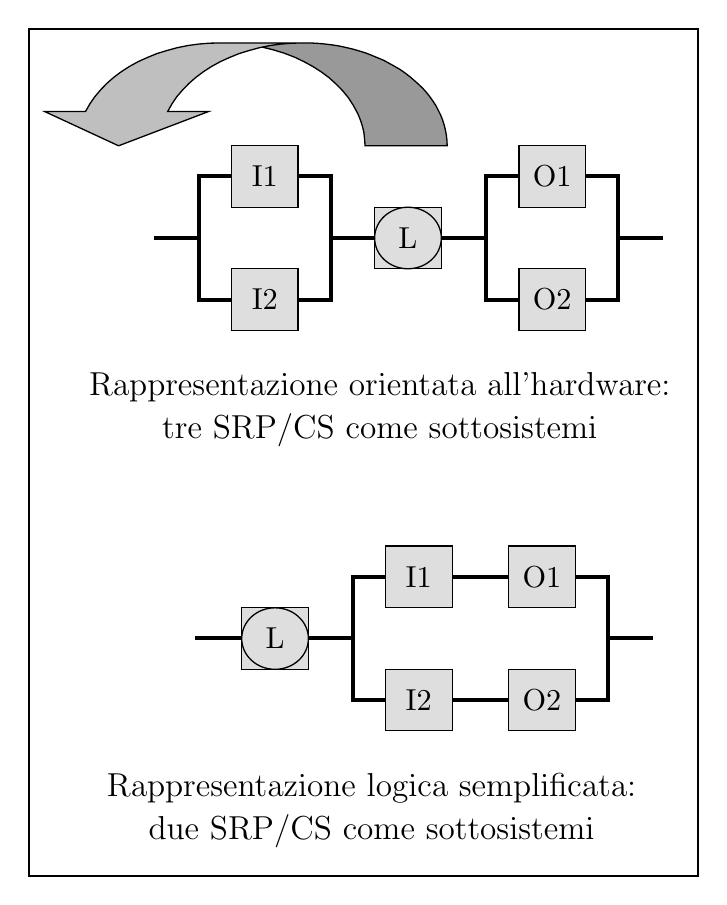
\begin{tikzpicture}[
  x=0.035cm, y=0.035cm,
  cornice/.style={draw=black, line width=0.75pt},
  blocco/.style={draw=black, fill=black!13, line width=0.47pt},
  collegamento/.style={draw=black, line width=1.49pt},
  sigla/.style={font=\fontsize{11.3}{13.5}\selectfont},
  dicitura/.style={font=\fontsize{13}{15.5}\selectfont, align=center}
]

\setstretch{1}

% --- freccia curva del riordino (conversione dai tracciati originali) ---
\fill[fill=black!25] (32.98,265.37) -- (65.7,277.83) -- (50.79,277.83) -- (52.37,280.6) -- (54.11,283.2) -- (56.23,285.64) -- (58.52,288.01) -- (61.05,290.22) -- (63.8,292.26) -- (66.72,294.16) -- (69.88,295.89) -- (73.19,297.39) -- (76.66,298.81) -- (80.28,299.92) -- (84,300.94) -- (87.86,301.73) -- (91.88,302.28) -- (95.9,302.6) -- (100,302.67) -- (70.19,302.67) -- (66.09,302.6) -- (62.07,302.28) -- (58.05,301.73) -- (54.18,300.94) -- (50.48,299.92) -- (46.85,298.81) -- (43.39,297.39) -- (40.07,295.89) -- (36.92,294.16) -- (34,292.26) -- (31.24,290.22) -- (28.72,288.01) -- (26.43,285.64) -- (24.38,283.2) -- (22.57,280.6) -- (20.99,277.83) -- (6.09,277.83) -- cycle;
\fill[fill=black!40] (85.1,301.18) -- (89.2,300.15) -- (93.06,298.97) -- (96.77,297.55) -- (100.24,295.89) -- (103.55,294.08) -- (106.62,292.11) -- (109.46,289.98) -- (111.99,287.69) -- (114.36,285.25) -- (116.4,282.73) -- (118.14,280.04) -- (119.63,277.28) -- (120.26,275.86) -- (120.81,274.44) -- (121.29,272.94) -- (121.68,271.53) -- (122,270.03) -- (122.16,268.45) -- (122.31,266.95) -- (122.39,265.37) -- (152.2,265.37) -- (152.12,267.35) -- (151.89,269.24) -- (151.57,271.05) -- (151.1,272.94) -- (150.54,274.76) -- (149.84,276.5) -- (148.96,278.23) -- (148.1,279.96) -- (147,281.62) -- (145.89,283.2) -- (144.63,284.78) -- (143.29,286.27) -- (141.79,287.69) -- (140.21,289.11) -- (138.64,290.45) -- (136.9,291.79) -- (135.09,293.06) -- (133.19,294.16) -- (129.17,296.37) -- (124.84,298.18) -- (122.63,299.05) -- (120.34,299.76) -- (117.9,300.47) -- (115.54,301.02) -- (113.01,301.57) -- (110.49,301.97) -- (107.96,302.28) -- (105.36,302.52) -- (102.68,302.67) -- (100,302.67) -- (96.21,302.6) -- (92.51,302.28) -- (88.73,301.81) -- cycle;
\draw[draw=black, line width=0.47pt] (85.1,301.18) -- (89.2,300.15) -- (93.06,298.97) -- (96.76,297.55) -- (100.24,295.89) -- (103.55,294.08) -- (106.62,292.11) -- (109.46,289.98) -- (111.98,287.69) -- (114.35,285.25) -- (116.4,282.73) -- (118.13,280.04) -- (119.63,277.28) -- (120.26,275.86) -- (120.82,274.44) -- (121.29,272.94) -- (121.68,271.53) -- (122,270.03) -- (122.16,268.45) -- (122.31,266.95) -- (122.39,265.37) -- (152.2,265.37) -- (152.12,267.35) -- (151.89,269.24) -- (151.57,271.05) -- (151.1,272.94) -- (150.54,274.76) -- (149.84,276.5) -- (148.1,279.96) -- (147,281.62) -- (145.89,283.2) -- (144.63,284.78) -- (143.29,286.27) -- (141.79,287.69) -- (140.21,289.11) -- (138.64,290.45) -- (136.9,291.79) -- (135.09,293.06) -- (133.19,294.16) -- (129.18,296.37) -- (124.84,298.18) -- (122.63,299.05) -- (120.34,299.76) -- (117.9,300.47) -- (115.53,301.02) -- (113.01,301.57) -- (110.48,301.97) -- (107.96,302.28) -- (105.36,302.52) -- (102.68,302.67) -- (70.19,302.67) -- (66.09,302.6) -- (62.07,302.28) -- (58.05,301.73) -- (54.18,300.94) -- (50.48,299.92) -- (46.85,298.81) -- (43.39,297.39) -- (40.07,295.89) -- (36.92,294.16) -- (34,292.27) -- (31.24,290.22) -- (28.72,288.01) -- (26.43,285.64) -- (24.38,283.2) -- (22.57,280.6) -- (20.99,277.83) -- (6.09,277.83) -- (32.98,265.37) -- (65.7,277.83) -- (50.79,277.83) -- (52.37,280.6) -- (54.11,283.2) -- (56.23,285.64) -- (58.52,288.01) -- (61.05,290.22) -- (63.8,292.27) -- (66.72,294.16) -- (69.88,295.89) -- (73.19,297.39) -- (76.66,298.81) -- (80.29,299.92) -- (84,300.94) -- (87.86,301.73) -- (91.88,302.28) -- (95.9,302.6) -- (100,302.67);

% ===================== schema in alto: tre sottosistemi =====================
% linee portanti
\draw[collegamento] (45.91,231.87) -- (62.78,231.87);
\draw[collegamento] (150.15,231.87) -- (167.02,231.87);
\draw[collegamento] (213.62,231.87) -- (230.50,231.87);
% staffe dei due canali
\draw[collegamento] (74.06,254.26) -- (62.15,254.26) -- (62.15,209.55) -- (74.06,209.55);
\draw[collegamento] (98.10,254.26) -- (109.94,254.26) -- (109.94,209.55) -- (98.10,209.55);
\draw[collegamento] (178.30,254.26) -- (166.39,254.26) -- (166.39,209.55) -- (178.30,209.55);
\draw[collegamento] (202.35,254.26) -- (214.18,254.26) -- (214.18,209.55) -- (202.35,209.55);
% tratto fra la staffa di ingresso e il blocco L
\draw[collegamento] (109.38,231.87) -- (125.86,231.87);
% blocchi
\draw[blocco] (73.98,243.07) rectangle (98.10,265.38);
\draw[blocco] (178.22,243.07) rectangle (202.35,265.38);
\draw[blocco] (73.98,198.35) rectangle (98.10,220.75);
\draw[blocco] (178.22,198.35) rectangle (202.35,220.75);
% sottosistema incapsulato: cerchio inscritto nel quadrato
\draw[blocco] (125.86,220.75) rectangle (150.07,243.07);
\draw[blocco] (137.97,231.91) ellipse [x radius=12.1, y radius=11.16];
% sigle
\node[sigla] at (86.04,254.22) {I1};
\node[sigla] at (190.29,254.22) {O1};
\node[sigla] at (137.97,231.91) {L};
\node[sigla] at (86.04,209.55) {I2};
\node[sigla] at (190.29,209.55) {O2};
% dicitura
\node[dicitura] at (127.73,169.62)
  {Rappresentazione orientata all'hardware:\\tre SRP/CS come sottosistemi};

% ================= schema in basso: due sottosistemi =================
\draw[collegamento] (60.81,86.63) -- (77.68,86.63);
\draw[collegamento] (101.81,86.63) -- (118.69,86.63);
\draw[collegamento] (209.92,86.63) -- (226.79,86.63);
\draw[collegamento] (154.01,108.93) -- (174.59,108.93);
\draw[collegamento] (154.01,64.23) -- (174.59,64.23);
\draw[collegamento] (129.81,108.94) -- (117.90,108.94) -- (117.90,64.23) -- (129.81,64.23);
\draw[collegamento] (198.64,108.94) -- (210.47,108.94) -- (210.47,64.23) -- (198.64,64.23);
% blocchi
\draw[blocco] (129.73,97.74) rectangle (154.01,120.13);
\draw[blocco] (174.51,97.74) rectangle (198.64,120.13);
\draw[blocco] (129.73,53.11) rectangle (154.01,75.42);
\draw[blocco] (174.51,53.11) rectangle (198.64,75.42);
\draw[blocco] (77.60,75.42) rectangle (101.89,97.74);
\draw[blocco] (89.75,86.58) ellipse [x radius=12.1, y radius=11.16];
% sigle
\node[sigla] at (141.87,108.93) {I1};
\node[sigla] at (186.58,108.93) {O1};
\node[sigla] at (89.75,86.58) {L};
\node[sigla] at (141.87,64.26) {I2};
\node[sigla] at (186.58,64.26) {O2};
% dicitura
\node[dicitura] at (124.73,24.12)
  {Rappresentazione logica semplificata:\\due SRP/CS come sottosistemi};

% --- cornice esterna --------------------------------------------------------
\draw[cornice] (0.37,0.37) rectangle (243.11,307.85);

\end{tikzpicture}
}
        \captionof{figure}{I sottosistemi misti possono essere riordinati nello schema a blocchi legato alla sicurezza, ad esempio dando la precedenza ai sottosistemi incapsulati (qui "L").}
        \label{fig:06-14}
    \end{minipage}
\end{center}

Un ulteriore caso particolare è l'integrazione, come blocchi in una SRP/CS, di sottosistemi che già possiedono un PL (o SIL) oppure una probabilità media di guasto pericoloso per ora PFH\textsubscript{D}. Come regola approssimativa, senza esaminare la struttura interna del sottosistema, il reciproco della probabilità media di guasto pericoloso per ora PFH\textsubscript{D} può essere sostituito come MTTF\textsubscript{D} del blocco. Poiché eventuali misure diagnostiche del sottosistema, se implementate internamente, sono già state considerate nella probabilità di guasto, per la DC del blocco possono essere considerate soltanto misure diagnostiche supplementari che agiscono esternamente sul sottosistema. Informazioni più dettagliate si trovano al punto 2 di [32]. Il punto 3 di questa pubblicazione tratta inoltre il caso in cui più di due canali funzionali siano collegati in parallelo.

Un'ulteriore questione che può presentarsi in questo contesto riguarda l'assegnazione di una categoria per un sistema completo, a sua volta costituito da sottosistemi per i quali l'unica informazione disponibile è la probabilità media di guasto pericoloso per ora PFH\textsubscript{D}. Oltre alle informazioni sulla struttura interna, in questo caso mancano anche le informazioni sull'MTTF\textsubscript{D} di ciascun canale e sulla DC\textsubscript{avg}, per le quali si applicano requisiti minimi in funzione della categoria. Vale pertanto lo stesso principio già visto per le disposizioni in parallelo: l'unica alternativa a una stima molto approssimativa è una nuova valutazione, eventualmente con lo sfruttamento dei risultati intermedi ottenuti.

\section{Determinazione del PL di una taglierina a ghigliottina}
\label{sec:06-5}
Il presente punto integra la descrizione generale con un'illustrazione di come il PL venga determinato nella pratica. Al tempo stesso, l'esempio qui descritto in dettaglio facilita l'accesso del lettore al Capitolo 8, che contiene un ampio numero di esempi circuitali per diversi PL, categorie e tipi di tecnologia.
I riquadri di testo con sfondo grigio riportati di seguito corrispondono alle brevi descrizioni nella forma utilizzata nel Capitolo 8. Sono inoltre fornite spiegazioni aggiuntive; il rimando a queste per ciascun esempio circuitale risulterebbe troppo dispersivo nel Capitolo 8

\subsection{Funzioni di sicurezza}
\label{subsec:06-5-1}
Si riprende qui l'esempio del sistema di comando di una taglierina a ghigliottina per carta descritto nella Figura 5.7. Tra le sette funzioni di sicurezza ivi indicate, viene descritta a titolo esemplificativo la realizzazione della SF2, per la quale il Performance Level richiesto era risultato essere PL\textsubscript{r} e. Poiché le diverse funzioni di sicurezza possono avvalersi degli stessi componenti, tutte le funzioni di sicurezza devono essere prese in considerazione durante la realizzazione. Ad esempio, per la protezione sul lato operatore, la norma di prodotto che disciplina le taglierine a ghigliottina per carta, la EN 1010-3, richiede, per la funzione di sicurezza SF3, un'apparecchiatura elettrosensibile di protezione (ESPE, non mostrata qui), in aggiunta a un comando bimanuale (THC).

\textit{Funzione di sicurezza (SF2)}:
\begin{itemize}
    \item posizionamento controllato delle mani dell'operatore al di fuori della zona pericolosa durante un movimento pericoloso
\end{itemize}

\subsection{Implementazione}
\label{subsec:06-5-2}
Qualora la realizzazione avvenga sotto forma di comando bimanuale, questa funzione di sicurezza può essere descritta come segue: quando almeno uno dei due attuatori S1 e S2 viene rilasciato, il movimento pericoloso della barra di pressione e della lama viene interrotto, ed entrambe - barra di pressione e lama - vengono riportate nella loro posizione iniziale per azione della forza delle molle. Un riavvio è impedito finché entrambi gli attuatori non siano stati rilasciati e non venga avviato un nuovo ciclo mediante il comando bimanuale. Il posizionamento controllato delle mani dell'operatore è ottenuto mediante due attuatori che devono essere azionati simultaneamente affinché la macchina possa essere avviata (per i dettagli, ad esempio riguardo all'immunità alla neutralizzazione, vedere EN 574). La temporizzazione e la logica dei segnali elettrici devono essere interpretate; un sistema di comando elettronico programmabile costituisce una soluzione idonea a tale scopo, e controllerà generalmente anche il movimento della barra di pressione e della lama. A causa delle elevate forze richieste, queste parti sono azionate idraulicamente. Come descritto nel Capitolo 5 (vedere punto 5.3.2), la funzione di sicurezza comprende entrambi gli attuatori - barra di pressione e lama - poiché si trovano nella stessa zona di pericolo. La Figura~\ref{fig:06-15} rappresenta uno schema elettroidraulico concettuale che mostra come le parti dei sistemi di comando legate alla sicurezza siano realizzate nella pratica. Come nel Capitolo 8, molti dettagli sono naturalmente stati omessi dallo schema qui riportato, nell'interesse di una maggiore chiarezza. Oltre alla maggior parte delle parti funzionali del sistema di comando necessarie per il funzionamento della macchina nell'ambito del processo, sono stati omessi dallo schema anche alcuni dettagli legati alla sicurezza, quali i circuiti di protezione (fusibili, CEM) e le "periferiche" (alimentazione, segnali di clock, ecc. per la logica). A causa della richiesta tolleranza al guasto singolo e della tolleranza a un accumulo di guasti non rilevati, nella pratica sono inoltre necessari, ad esempio, elementi di disaccoppiamento tra gli ingressi interconnessi dei due canali logici, affinché un ingresso difettoso su un canale non provochi interferenze sull'altro canale. Occorre pertanto tenere presente che uno schema concettuale come questo non costituisce una documentazione dalla quale sarebbe possibile realizzare una replica; il suo scopo è piuttosto quello di illustrare la struttura della tecnica di sicurezza.

\subsection{Descrizione funzionale}
\label{subsec:06-5-3}
Una descrizione funzionale che illustri la struttura del circuito e i percorsi dei segnali è essenziale per la comprensione dello schema circuitale. Essa è finalizzata a consentire l'identificazione del processo funzionale durante l'esecuzione della funzione di sicurezza (che può svolgersi in canali diversi) e delle misure di test realizzate.

% La minipage tiene insieme disegno e didascalia (figura non fluttuante)
\begin{center}
    \begin{minipage}{\textwidth}
        \centering
        \captionsetup{hypcap=false}
        \resizebox{0.92\textwidth}{!}{%==============================================================
%  Figura 6.15 - Schema di principio dell'azionamento elettronico di
%  una lama idraulica e di una barra di pressione idraulica
%  Adattamento in italiano della Figura 6.15 dell'IFA Report 2/2017
%
%  Nell'originale questa figura e' un'immagine raster incorporata che
%  contiene SOLO il disegno: tutte le scritte (diciture e sigle dei
%  componenti) stanno in un livello di testo separato. Qui si fa
%  altrettanto: img06-15.png e' il disegno estratto dall'originale
%  (pagina 76 di rep0217e.pdf, 1877x2776 px a 300 ppi) e le scritte
%  sono nodi TikZ sovrapposti, quindi restano testo selezionabile e
%  sono state tradotte senza ritoccare il bitmap.
%
%  Le posizioni dei nodi sono quelle misurate nell'originale.
%  Sistema di riferimento: l'origine e' l'angolo in basso a sinistra
%  della cornice, l'asse y e' rivolto verso l'alto e una unita' e' un
%  punto PostScript del disegno originale.
%==============================================================
\begin{tikzpicture}[
  x=0.035cm, y=0.035cm,
  grande/.style={font=\fontsize{10.2}{12}\selectfont},
  media/.style={font=\fontsize{8.5}{10}\selectfont},
  piccola/.style={font=\fontsize{7.6}{9}\selectfont}
]

\setstretch{1}

% --- disegno (bitmap estratto dall'originale, privo di scritte) ---
\node[anchor=south west, inner sep=0] at (22.69,6.39)
  {
\includegraphics[width=15.740cm, height=23.289cm]{img06-15.png}};

% --- scritte: diciture tradotte e sigle dei componenti ---
\node[grande] at (153.06,661.35) {Azionamento della lama};
\node[grande] at (385.72,661.35) {Barra di pressione};
\node[media] at (121.89,641.37) {1A};
\node[media] at (348.32,641.37) {2A};
\node[grande, align=center] at (225.54,596.72) {Movimento\\pericoloso};
\node[grande, align=center] at (446.75,596.72) {Movimento\\pericoloso};
\node[media] at (290.19,578.77) {K4};
\node[media] at (64.14,577.83) {K3};
\node[media] at (62.25,561.48) {1V4};
\node[media] at (288.83,560.08) {2V2};
\node[media] at (54.92,533.22) {P};
\node[media] at (270.05,533.22) {P};
\node[media] at (39.65,530.42) {1S3};
\node[media] at (251.99,528.78) {2S1};
\node[media] at (290.24,504.02) {K6};
\node[media] at (63.93,486.97) {1V3};
\node[media] at (288.66,486.97) {2V1};
\node[media] at (177.03,471.55) {1V5};
\node[media] at (326.88,471.55) {2V3};
\node[media] at (61.86,463.85) {K5};
\node[media] at (152.71,424.61) {1V2};
\node[media] at (117.51,391.91) {1V1};
\node[media] at (213.40,389.80) {1Z2};
\node[media] at (347.14,364.27) {1Z1};
\node[media] at (62.67,350.80) {M};
\node[media] at (288.65,347.29) {1S1};
\node[media] at (319.81,347.29) {1S2};
\node[media] at (39.70,344.56) {1M};
\node[media] at (164.79,344.56) {1P};
\node[media] at (58.55,340.52) {3};
\node[media] at (68.19,273.17) {+};
\node[media] at (88.51,273.17) {+};
\node[media] at (151.73,273.17) {+};
\node[media] at (183.81,273.17) {+};
\node[media] at (294.06,273.17) {+};
\node[media] at (315.39,273.17) {+};
\node[media] at (378.29,273.17) {+};
\node[media] at (409.43,273.17) {+};
\node[media] at (125.76,254.49) {1S3};
\node[media] at (351.97,254.48) {2S1};
\node[media] at (175.14,250.75) {K5};
\node[media] at (402.66,249.50) {K3};
\node[piccola] at (76.90,245.46) {13};
\node[piccola] at (305.03,245.15) {13};
\node[piccola] at (100.28,244.84) {21};
\node[piccola] at (328.41,244.53) {21};
\node[grande] at (125.81,240.14) {P\textgreater{}};
\node[grande] at (351.92,240.14) {P\textgreater{}};
\node[media] at (40.98,239.54) {S1};
\node[media] at (268.03,239.54) {S2};
\node[piccola] at (77.07,233.63) {14};
\node[piccola] at (100.86,233.63) {22};
\node[piccola] at (305.19,233.32) {14};
\node[piccola] at (328.98,233.32) {22};
\node[media] at (175.54,219.61) {K6};
\node[media] at (402.86,218.35) {K4};
\node[media] at (45.39,127.10) {K1};
\node[media] at (272.53,127.10) {K2};
\node[media] at (348.66,125.24) {Ingresso};
\node[media] at (116.32,125.24) {Ingresso};
\node[grande] at (352.38,104.97) {ASIC};
\node[grande] at (121.69,103.73) {Microcontrollore};
\node[media, align=center] at (239.52,102.35) {Sincronizzazione e\\scambio di dati};
\node[media] at (119.66,78.83) {Uscita};
\node[media] at (351.99,78.83) {Uscita};
\node[media] at (115.49,61.40) {1V4};
\node[media] at (174.54,61.39) {2V2};
\node[media] at (342.68,61.39) {1V3};
\node[media] at (399.69,61.39) {2V1};
\node[media] at (134.62,34.61) {K4};
\node[media] at (74.35,34.60) {K3};
\node[media] at (302.22,34.60) {K5};
\node[media] at (360.56,34.60) {K6};

% --- cornice esterna ---
\draw[draw=black, line width=0.75pt] (0.37,0.37) rectangle (497.93,677.81);

\end{tikzpicture}
}
        \captionof{figure}{Schema di principio dell'azionamento elettronico di una lama idraulica e di una barra di pressione idraulica (componenti essenziali).}
        \label{fig:06-15}
    \end{minipage}
\end{center}

\textbf{Descrizione funzionale}
\begin{itemize}
    \item l'azionamento degli attuatori S1 e S2 del comando bimanuale avvia i movimenti pericolosi (ciclo di lavorazione) della barra di pressione e della lama. Qualora uno dei due attuatori del comando bimanuale venga rilasciato durante questo ciclo, oppure si verifichi una variazione di segnale nel sistema periferico della macchina non attesa dal sistema di comando, il ciclo viene interrotto e la macchina assume lo stato sicuro;
    \item la pressione degli attuatori S1 e S2 fa sì che i fronti di salita dei segnali vengano inviati ai due canali di elaborazione K1 (microcontrollore) e K2 (ASIC). A condizione che tali segnali soddisfino i requisiti di simultaneità (500 ms) secondo la pertinente norma EN 574, i due canali di elaborazione impostano le uscite (relè a contattore K3-K6) per una richiesta di taglio valida;
    \item i due canali di elaborazione operano in modo sincrono e valutano inoltre reciprocamente gli stati intermedi interni delle operazioni cicliche di elaborazione dei segnali. Scostamenti dagli stati intermedi definiti causano l'arresto della macchina. Un canale di elaborazione è costituito da un microcontrollore (K1), l'altro da un ASIC (K2). K1 e K2 eseguono autotest in background durante il funzionamento;
    \item i guasti negli attuatori S1/S2 e nei relè a contattore K3-K6 (con contatti di riscontro meccanicamente collegati) sono rilevati mediante monitoraggio incrociato nei canali di elaborazione;
    \item il guasto delle valvole 1V3/1V4 e 2V1/2V2 è rilevato mediante i pressostati 1S3 e 2S1.
    \item il guasto delle valvole, o il blocco in posizione aperta di 1V4 o 2V2, è rilevato tramite una forte riduzione della velocità di ritorno dei cilindri idraulici. Questa situazione può essere rilevata anche dal sistema di comando mediante un'opportuna interpretazione dei segnali di pressione (durata della caduta di pressione);
    \item il guasto delle valvole, o il blocco in posizione aperta di 1V3 o 2V1, è rilevato direttamente mediante il monitoraggio della variazione di segnale dei pressostati 1S3 e 2S1: qualora una valvola resti bloccata, viene segnalata una pressione anche quando non dovrebbe essere presente alcuna pressione;
    \item tutti gli stati della macchina sono monitorati da entrambi i canali di elaborazione. La natura ciclica dell'operazione di taglio fa sì che tutti gli stati del sistema vengano percorsi ciclicamente, consentendo così il rilevamento dei guasti."
\end{itemize}

\subsection{Schema a blocchi legato alla sicurezza}
\label{subsec:06-5-4}
La descrizione della struttura circuitale, unitamente allo schema elettrico e, ove applicabile, ad altri documenti descrittivi (specifica esaustiva), consente di determinare una categoria di comando e di ricondurre il circuito effettivo a uno schema a blocchi legato alla sicurezza in forma astratta (Figura 6.16, pag. 78). Da questo esempio risulta rapidamente evidente che la funzione di sicurezza è eseguita in modalità a due canali. Possono pertanto essere prese in considerazione la categoria 3 o la categoria 4. Le misure di test di alta qualità, mediante le quali possono essere controllate anche le combinazioni di guasti, fanno propendere per la categoria 4. Ciò viene dimostrato esplicitamente dalla fase di verifica nel Capitolo 7, così come la verifica dei requisiti quantitativi relativi a MTTF\textsubscript{D}, DC\textsubscript{avg} e CCF (vedere oltre). Le spiegazioni fornite ai punti 6.2.8 e 6.2.9 sono utili per la realizzazione dello schema a blocchi legato alla sicurezza. Una procedura collaudata consiste nel seguire il percorso del segnale, iniziando dal lato attuatore, ponendosi la domanda: "Come viene azionato/impedito il movimento pericoloso?", per poi seguire la logica a ritroso fino ai sensori. Il SISTEMA Cookbook 1 [34] descrive questo passaggio, "Dallo schema circuitale al Performance Level", in maggiore dettaglio.

Si noti, in questo esempio, che gli attuatori S1 e S2 non sono ridondanti tra loro, anche se a prima vista potrebbero sembrarlo, poiché ciascun pulsante protegge indipendentemente una delle mani dell'utilizzatore. La ridondanza inizia piuttosto all'interno di ciascun pulsante, con l'impiego di combinazioni di contatti elettrici di apertura/di chiusura. Ciascun canale di comando monitora entrambe le mani/attuatori interpretando almeno un contatto elettrico di commutazione in ciascun attuatore. Lo schema a blocchi legato alla sicurezza contiene pertanto, in ciascun canale, un contatto di chiusura, ad es. S1/13-14, e un contatto di apertura, ad es. S2/21-22. Lo schema a blocchi legato alla sicurezza differisce sotto questo aspetto in modo sostanziale dallo schema elettrico funzionale.

In determinate circostanze, la realizzazione effettiva della funzione di sicurezza può comportare restrizioni o raccomandazioni per l'applicazione. Ad esempio, l'efficacia del rilevamento dei guasti attraverso il processo di lavorazione è per definizione strettamente legata all'applicazione.

\subsection{Grandezze di ingresso per la valutazione quantitativa del PL raggiunto}
\label{subsec:06-5-5}
A questo punto sono disponibili tutte le informazioni di base per la valutazione del PL raggiunto. Conoscendo la Categoria e lo schema a blocchi relativo alla sicurezza, è possibile determinare innanzitutto l'MTTF\textsubscript{D} e la DC dei singoli blocchi e valutare, per le ridondanze presenti, le misure contro i guasti di causa comune (CCF).

\textbf{Calcolo della probabilità di guasto}:
\begin{itemize}
    \item MTTF\textsubscript{D}: con 240 giorni lavorativi all'anno, 8 ore lavorative al giorno e un tempo di ciclo di 80 secondi, n\textsubscript{op} risulta pari a 86.400 cicli all'anno. Per S1 e S2 e per K3-K6, un valore di B\textsubscript{10D} pari a 2.000.000 di cicli [M] produce un MTTF\textsubscript{D} di 232 anni. Per il solo microcontrollore viene determinato un MTTF\textsubscript{D} di 1.142 anni [D]. Lo stesso valore viene sostituito anche per l'ASIC [D]. Insieme alla relativa disposizione circuitale, ciò dà luogo, in entrambi i casi, a un MTTF\textsubscript{D} di 806 anni per i blocchi K1 e K2. Il fabbricante indica un MTTF\textsubscript{D} di 150 anni [M] per ciascuna delle valvole idrauliche 1V3, 1V4, 2V1 e 2V2. Questi valori producono un MTTF\textsubscript{D} per ciascun canale pari a 31,4 anni ("alto");
    \item DC\textsubscript{avg}: conformemente all'Allegato E della EN ISO 13849-1, i valori di DC ottenuti sono: per S1/S2: 99\% (monitoraggio incrociato dei segnali di ingresso senza test dinamico con variazione frequente del segnale); per K1/K2: 90\% (autotest tramite software e monitoraggio incrociato); per K3-K6: 99\% (monitoraggio diretto mediante contatti meccanicamente collegati); per 1V3/2V1: 99\% (monitoraggio indiretto tramite il sensore di pressione); e per 1V4/2V2: 99\% (monitoraggio indiretto tramite la funzione e la misura di una variazione della durata della caduta di pressione). Questi valori danno luogo a una DC\textsubscript{avg} del 98,6\% ("alta");
    \item misure adeguate contro i guasti per causa comune (65 punti): separazione (15), protezione da sovratensione ecc. (15) e condizioni ambientali (25 + 10);
    \item la combinazione degli elementi di comando soddisfa la categoria 4 con un MTTF\textsubscript{D} per canale alto (31,4 anni) e una DC\textsubscript{avg} del 98,6\%, entro la fascia di tolleranza "alta". Ne risulta una probabilità media di guasto pericoloso di 9,7 10\textsuperscript{-8} all'ora. Ciò soddisfa il PL e;
\end{itemize}

Per chiarire il calcolo dell'MTTF\textsubscript{D} si considera anzitutto il blocco "K1": sebbene lo schema concettuale (Figura 6.15) mostri soltanto il microcontrollore, questo blocco comprende ulteriori elementi necessari per la funzionalità pratica (ad es. l'oscillatore al quarzo). Devono essere considerati tutti gli elementi il cui guasto pericoloso potrebbe impedire l'esecuzione della funzione di sicurezza nel canale interessato. Ciò comprende generalmente tutti gli elementi presenti nel percorso del segnale critici per la sicurezza, ad esempio per il disaccoppiamento, il riscontro, la protezione CEM o la protezione contro la sovratensione. Questi elementi sono generalmente necessari per la realizzazione dei principi di sicurezza di base e ben collaudati o per il raggiungimento della DC. La Figura B.2 (vedere pag. 253) illustra questo approccio con riferimento a un ulteriore esempio semplice. 

Il metodo del conteggio dei componenti (parts count) mostrato nella Tabella~\ref{tab:06-8} è adatto come semplice metodo tabellare per determinare l'MTTF\textsubscript{D} del blocco a partire dall'MTTF\textsubscript{D} dei singoli elementi. (Per confronto, la Figura B.3 a pag. 255 mostra la procedura per un'analisi dei modi di guasto e dei loro effetti.)

I tassi di guasto degli elementi indicati nella seconda colonna sono stati determinati mediante la banca dati SN 29500 [49], come indicato dal codice [D] alla voce "calcolo della probabilità di guasto" (vedere punto 7.6). La convalida è descritta più in dettaglio nel seguito di questo esempio, al punto 7.6. Poiché elementi identici possono comparire più volte (terza colonna), il tasso di guasto complessivo per ciascun tipo di elemento viene calcolato e indicato nella quarta colonna. L'approssimazione generale secondo cui soltanto la metà dei guasti è pericolosa produce il valore dimezzato riportato nella colonna 5. Infine, una semplice sommatoria produce il tasso complessivo di guasti pericolosi per il blocco K1. La colonna 6 mostra i corrispondenti valori di MTTF\textsubscript{D} in anni, ricavati come reciproci dei tassi di guasto pericoloso (dalla colonna 5, dopo la conversione da ore ad anni). Questo valore è arrotondato a 806 anni per il blocco K1. Poiché la banca dati impiegata indica tassi di guasto identici per il microcontrollore e per l'ASIC, e il circuito è analogo, il valore di MTTF\textsubscript{D} di 806 anni si applica anche al blocco K2.

% Tabella non fluttuante (minipage + \captionof): a fine capitolo un float
% finirebbe da solo su una pagina a parte.
%
% La quinta colonna e' riquadrata in grassetto perche' e' quella che alimenta
% il totale: filetti verticali spessi nel preambolo (!{\vrule width 1.2pt}) e
% tratti orizzontali spessi sopra e sotto con \cmidrule[1.2pt]{5-5}.
% La barra del totale e' una seconda tabularx con le stesse larghezze di
% colonna, cosi' i due valori restano incolonnati con quelli di sopra.
\begin{center}
    \begin{minipage}{\textwidth}
    \captionsetup{hypcap=false}
    \definecolor{tabblue}{RGB}{31,73,125}
    \setlength{\tabcolsep}{3pt}
    \renewcommand{\arraystretch}{1.25}
    \setstretch{1}
    \footnotesize
    % frecce del riepilogo
    \newcommand{\frecciagiu}{\tikz[baseline=-0.4ex]{\fill
        (-0.09,0.30) -- (0.09,0.30) -- (0.09,0.06) -- (0.20,0.06) --
        (0,-0.16) -- (-0.20,0.06) -- (-0.09,0.06) -- cycle;}}
    \newcommand{\frecciadx}{\tikz[baseline=-0.5ex]{\fill
        (-0.30,-0.09) -- (-0.30,0.09) -- (-0.06,0.09) -- (-0.06,0.20) --
        (0.16,0) -- (-0.06,-0.20) -- (-0.06,-0.09) -- cycle;}}
    \captionof{table}{Metodo del conteggio dei componenti (\textit{parts count}) per il blocco "microcontrollore" K1, sulla base dei tassi di guasto $\lambda$ tratti dalla raccolta di dati SN~29500~\cite{sn29500} (espressi in FIT, ossia $10^{-9}$ all'ora).}
    \label{tab:06-8}

    \begin{tabularx}{\textwidth}{%
        |>{\raggedright\arraybackslash}p{5.7cm}%
        |>{\centering\arraybackslash}p{2.3cm}%
        |>{\centering\arraybackslash}p{1.3cm}%
        |>{\centering\arraybackslash}p{1.9cm}%
        !{\vrule width 1.2pt}>{\centering\arraybackslash}p{2.0cm}%
        !{\vrule width 1.2pt}|C|}
        \hline
        \cmidrule[1.2pt]{5-5}
        \rowcolor{tabblue}
        \textcolor{white}{\textbf{Componente}} &
        \textcolor{white}{\textbf{Tasso di guasto $\lambda$ in FIT secondo la SN~29500}} &
        \textcolor{white}{\textbf{Numero}} &
        \textcolor{white}{\textbf{Tasso di guasto totale $\lambda$ in FIT}} &
        \textcolor{white}{\textbf{Tasso totale di guasti pericolosi $\lambda_{\mathrm{D}}$ in FIT}} &
        \textcolor{white}{\textbf{\textit{MTTF}\textsubscript{D} in anni come reciproco di $\lambda_{\mathrm{D}}$}} \\
        \hline
        Resistore a film metallico        & 0,2 & 7 & 1,4 & 0,7 & 163.079 \\
        \hline
        \rowcolor{black!8}
        Condensatore, non alimentato      & 1   & 4 & 4   & 2   & 57.078 \\
        \hline
        Diodo per impieghi generali       & 1   & 3 & 3   & 1,5 & 76.104 \\
        \hline
        \rowcolor{black!8}
        Optoaccoppiatore, uscita bipolare & 15  & 2 & 30  & 15  & 7.610 \\
        \hline
        Microcontrollore                  & 200 & 1 & 200 & 100 & 1.142 \\
        \hline
        \rowcolor{black!8}
        Oscillatore al quarzo             & 15  & 1 & 15  & 7,5 & 15.221 \\
        \hline
        Transistor bipolare, bassa potenza & 20 & 1 & 20  & 10  & 11.416 \\
        \hline
        \rowcolor{black!8}
        Relè con incapsulamento in plastica & 10 & 1 & 10 & 5   & 22.831 \\
        \hline
        \cmidrule[1.2pt]{5-5}
    \end{tabularx}

    % freccia verso il basso, incolonnata sotto la quinta colonna
    \vspace{2pt}
    \begin{tabularx}{\textwidth}{%
        @{}p{5.7cm}@{}p{2.3cm}@{}p{1.3cm}@{}p{1.9cm}%
        @{}>{\centering\arraybackslash}p{2.0cm}@{}X@{}}
        & & & & \frecciagiu & \\
    \end{tabularx}

    \vspace{2pt}
    \begin{tabularx}{\textwidth}{%
        |>{\raggedright\arraybackslash}p{5.7cm}%
        |>{\centering\arraybackslash}p{2.3cm}%
        |>{\centering\arraybackslash}p{1.3cm}%
        |>{\centering\arraybackslash}p{1.9cm}%
        |>{\centering\arraybackslash}p{2.0cm}|C|}
        \hline
        \rowcolor{black!8}
        \multicolumn{4}{|>{\raggedright\arraybackslash}p{11.62cm}|}{Totale per il blocco "microcontrollore" K1} &
        \fbox{141,7 FIT} &
        \frecciadx\enspace\fbox{806 anni} \\
        \hline
    \end{tabularx}
    \end{minipage}
\end{center}

Per i blocchi S1/S2 e K3-K6 sono utilizzati i dati dei fabbricanti ("[M]"). Poiché i dati di affidabilità sono disponibili soltanto per S1/S2 nel loro complesso (meccanismo di azionamento e contatto di apertura e di chiusura), questi valori possono essere utilizzati come stima a favore della sicurezza per ciascuno dei canali, anche se in ciascun canale vengono considerati soltanto i contatti di chiusura (ad es. S1/13-14) oppure i contatti di apertura (ad es. S2/21-22), oltre al meccanismo di azionamento. I valori di B\textsubscript{10D} assunti vengono convertiti in valori di MTTF\textsubscript{D} mediante le formule già note dall'Allegato D:

\begin{equation}
    n_{\mathrm{op}}
    = \frac{d_{\mathrm{op}} \cdot h_{\mathrm{op}}}{t_{\mathrm{ciclo}}} \cdot 3{.}600\,\frac{\mathrm{s}}{\mathrm{h}}
    = \frac{240\ \text{giorni/anno} \cdot 8\ \text{h/giorno}}{80\ \text{s/ciclo}} \cdot 3{.}600\,\frac{\mathrm{s}}{\mathrm{h}}
    = 86{.}400\,\frac{\text{cicli}}{\text{anno}}
    \label{eq:06-06}
\end{equation}

\begin{equation}
    \textit{MTTF}_{\mathrm{D}}
    = \frac{B_{\mathrm{10D}}}{0{,}1 \cdot n_{\mathrm{op}}}
    = \frac{2{.}000{.}000\ \text{cicli}}{0{,}1 \cdot 86{.}400\ \text{cicli/anno}}
    = 231{,}5\ \text{anni}
    \label{eq:06-07}
\end{equation}

La durata di funzionamento dei componenti elettromeccanici è limitata al valore T\textsubscript{10D} (tempo dopo il quale il 10\% dei componenti oggetto dell'analisi si è guastato in modo pericoloso). Poiché tuttavia, in questo caso, il valore di T\textsubscript{10D} è superiore al tempo di missione assunto di 20 anni, esso non è rilevante ai fini dell'ulteriore analisi. Dato che in:

\begin{equation}
    T_{\mathrm{10D}}
    = \frac{B_{\mathrm{10D}}}{n_{\mathrm{op}}}
    = \frac{2{.}000{.}000\ \text{cicli}}{86{.}400\ \text{cicli/anno}}
    = 23{,}2\ \text{anni}
    \label{eq:06-08}
\end{equation}

Il fabbricante indica inoltre un MTTF\textsubscript{D} di 150 anni [M] per ciascuna delle valvole idrauliche 1V3, 1V4, 2V1 e 2V2. Conformemente al punto 6.2.13, il totale per un canale (S1, S2, K1, K3, K4, 1V4, 2V2) produce un MTTF\textsubscript{D} di 31,4 anni, ossia "alto"."

% a corpo pieno la formula riempie tutta la riga e spinge il numero a capo:
% \small la stringe quel tanto che basta perche (9) resti in linea
{\small
\begin{equation}
    \frac{1}{\textit{MTTF}_{\mathrm{D}}}
    = \frac{1}{232\ \text{anni}} + \frac{1}{232\ \text{anni}} + \frac{1}{806\ \text{anni}}
    + \frac{1}{232\ \text{anni}} + \frac{1}{232\ \text{anni}} + \frac{1}{150\ \text{anni}}
    + \frac{1}{150\ \text{anni}}
    = \frac{1}{31{,}4\ \text{anni}}
    \label{eq:06-09}
\end{equation}
}

Poiché il secondo canale presenta lo stesso MTTF\textsubscript{D}, non è necessaria la simmetrizzazione, come sarebbe altrimenti il caso. Anche la convalida dei valori di DC assunti è descritta più in dettaglio nel Capitolo 7. Autotest di alta qualità, ad esempio, vengono eseguiti per K1 e K2 mediante software e monitoraggio incrociato, comprese le misure speciali per la memoria variante e invariante e per l'unità di elaborazione, richieste per i sistemi a microprocessore. Nel complesso, per la SRP/CS si ottiene, conformemente al punto 6.2.14, una DC\textsubscript{avg} del 98,6\%. Sfruttando la tolleranza del 5\%, questo valore rientra nella fascia "alta".


% formula molto larga (14 frazioni): \small la fa stare nella giustezza
{\small
\begin{equation}
    \textit{DC}_{\mathrm{avg}}
    = \frac{2 \cdot \left(
        \dfrac{99\%}{232\ \text{anni}} + \dfrac{99\%}{232\ \text{anni}}
        + \dfrac{90\%}{806\ \text{anni}} + \dfrac{99\%}{232\ \text{anni}}
        + \dfrac{99\%}{232\ \text{anni}} + \dfrac{99\%}{150\ \text{anni}}
        + \dfrac{99\%}{150\ \text{anni}}
      \right)}
      {2 \cdot \left(
        \dfrac{1}{232\ \text{anni}} + \dfrac{1}{232\ \text{anni}}
        + \dfrac{1}{806\ \text{anni}} + \dfrac{1}{232\ \text{anni}}
        + \dfrac{1}{232\ \text{anni}} + \dfrac{1}{150\ \text{anni}}
        + \dfrac{1}{150\ \text{anni}}
      \right)}
    = 98{,}6\%
    \label{eq:06-10}
\end{equation}
}

Le misure contro i guasti per causa comune (CCF) indicate nel riquadro grigio a pag. 78 sono in gran parte autoesplicative. La convalida è comunque descritta più in dettaglio nel Capitolo 7. Inoltre, la misura "diversità" e la misura "impiego di componenti ben collaudati" trovano applicazione rispettivamente nel sottosistema elettrico e in quello idraulico (vedere Allegato F). Con la soddisfazione dei requisiti relativi ai CCF, una DC\textsubscript{avg} "alta" e un MTTF\textsubscript{D} "alto", risultano soddisfatti anche i requisiti quantitativi della categoria 4.

\subsection{Diversi approcci per il calcolo del PL}
\label{subsec:06-5-6}
La determinazione del PL sulla base degli aspetti quantificabili è ormai quasi completa a questo punto. I risultati relativi a categoria, DC\textsubscript{avg} e MTTF\textsubscript{D} possono essere utilizzati per una conferma grafica, mediante il diagramma a barre, del fatto che venga raggiunto il PL e (vedere Figura~\ref{fig:06-17}). I valori tabellari dell'Allegato K della norma, o il calcolatore a disco PLC dell'IFA [16] basato su di essi, forniscono il seguente risultato:
\begin{center}
    \begin{minipage}{\textwidth}
    \captionsetup{hypcap=false}
    \centering
    \definecolor{tabblue}{RGB}{31,73,125}
    \setlength{\tabcolsep}{4pt}
    \renewcommand{\arraystretch}{1.25}
    \setstretch{1}
    \captionof{table}{Riepilogo delle grandezze di ingresso e del PL raggiunto dal sistema di comando della taglierina a ghigliottina.}
    \label{tab:06-9}

    \begin{tabular}{%
        |>{\centering\arraybackslash}p{2.1cm}%
        |>{\centering\arraybackslash}p{1.4cm}%
        |>{\centering\arraybackslash}p{2.0cm}%
        |>{\centering\arraybackslash}p{3.2cm}%
        |>{\centering\arraybackslash}p{4.4cm}|}
        \hline
        \rowcolor{tabblue}
        \textcolor{white}{\textbf{Categoria}} &
        \textcolor{white}{\textbf{CCF}} &
        \textcolor{white}{\textbf{\textit{DC}\textsubscript{avg}}} &
        \textcolor{white}{\textbf{\textit{MTTF}\textsubscript{D}}} &
        \textcolor{white}{\textbf{\textit{PFH}\textsubscript{D}}}
        \tabularnewline
        \hline
        4 & OK & "alta" &
        "alto" \newline (arrotondato per difetto: 30~anni) &
        \cellcolor{black!8} $9{,}5 \cdot 10^{-8}$ all'ora \newline (PL~e)
        \tabularnewline
        \hline
    \end{tabular}
    \end{minipage}
\end{center}

% La minipage tiene insieme disegno e didascalia (figura non fluttuante)
\begin{center}
    \begin{minipage}{\textwidth}
        \centering
        \captionsetup{hypcap=false}
        \resizebox{0.92\textwidth}{!}{%==============================================================
%  Figura 6.17 - Determinazione del PL mediante il diagramma
%  a barre / il disco di calcolo PLC
%  Adattamento in italiano della Figura 6.17 dell'IFA Report 2/2017
%  (pagina 80 di rep0217e.pdf)
%
%  Il diagramma a barre riusa il sistema di riferimento della
%  Figura 6.10 (immagini/fig06-10.tex): stesse coordinate in punti
%  PostScript dell'originale, unita' della tikzpicture x=y=0.042cm,
%  origine nell'angolo in basso a sinistra del riquadro del grafico.
%  Il riquadro sovrapposto riproduce il disco PLC dell'IFA; i marchi
%  (IFA, ZVEI, VDMA) sono resi in forma testuale semplificata.
%==============================================================
\begin{tikzpicture}[
  x=0.042cm, y=0.042cm,
  font=\small,
  cornice/.style={draw=black, line width=0.9pt},
  riquadro/.style={draw=black, line width=1.06pt},
  griglia/.style={draw=black, line width=1.06pt,
                  dash pattern=on 4.24pt off 2.12pt},
  tacca/.style={draw=black, line width=1.06pt},
  separatore/.style={draw=black, line width=0.8pt},
  contorno/.style={draw=black, line width=0.8pt},
  puntini/.style={draw=black, line width=0.52pt, line cap=butt,
                  dash pattern=on 0.53pt off 1.05pt},
  tratti/.style={draw=black, line width=0.52pt},
  etichetta/.style={draw=black, fill=black!15, line width=1.06pt,
                    rounded corners=2.9pt, inner sep=0pt, align=center},
  evidenza/.style={draw=black!55, fill=white, line width=1.2pt,
                   rounded corners=3.5pt, inner sep=0pt, align=center},
  fumetto/.style={draw=black, fill=white, line width=1.1pt,
                  inner sep=2pt, align=center},
  passo/.style={circle, fill=black!42, inner sep=0pt, align=center},
  frecciagrigia/.style={draw=black!42, line width=7pt,
                        -{Triangle[length=10pt, width=13pt]}},
  tratteggiata/.style={draw=black, line width=1.7pt,
                       dash pattern=on 6pt off 4pt,
                       -{Triangle[length=8pt, width=8pt]}}
]

\setstretch{1}

% --- riempimenti delle barre ------------------------------------------
\def\riempipuntini#1#2#3#4{%
  \begin{scope}
    \clip (#1,#2) rectangle (#3,#4);
    \foreach \k in {0,...,20}{%
      \draw[puntini] (#1,{#4-1.1-2.2155*\k}) -- (#3,{#4-1.1-2.2155*\k});}
  \end{scope}}
\def\riempitratti#1#2#3#4{%
  \begin{scope}
    \clip (#1,#2) rectangle (#3,#4);
    \foreach \k in {0,...,34}{%
      \draw[tratti] (#1,{#2-(#4-#2)+3.13*\k})
        -- ++({(#3-#1)+(#4-#2)},{(#3-#1)+(#4-#2)});}
  \end{scope}}
\def\barrabassa#1#2#3#4{%
  \fill[white] (#1,#2) rectangle (#3,#4);
  \riempipuntini{#1}{#2}{#3}{#4}
  \draw[contorno] (#1,#2) rectangle (#3,#4);}
\def\barramedia#1#2#3#4{%
  \fill[white] (#1,#2) rectangle (#3,#4);
  \riempitratti{#1}{#2}{#3}{#4}
  \draw[contorno] (#1,#2) rectangle (#3,#4);}
\def\barraalta#1#2#3#4{%
  \fill[black] (#1,#2) rectangle (#3,#4);
  \draw[contorno] (#1,#2) rectangle (#3,#4);}

% --- colonna delle PFHD a sinistra --------------------------------------
\draw[black!15, line width=6.62pt] (-38.64,211.73) -- (-38.64,0.44);

\node[etichetta, minimum width=1.4423cm, minimum height=1.1726cm]
  at (-38.81,218.58) {\textit{PFH}$_{\mathrm{D}}$\\(1/h)};

\foreach \yv/\testo in {175.89/{$10^{-4}$}, 140.50/{$10^{-5}$},
                        105.15/{$3\cdot 10^{-6}$}, 70.05/{$10^{-6}$},
                        34.87/{$10^{-7}$}, 0/{$10^{-8}$}}{%
  \draw[tacca] (-23.86,\yv) -- (-2.81,\yv);
  \node[etichetta, minimum width=1.4423cm, minimum height=0.5586cm]
    at (-38.81,\yv) {\testo};}

% --- asse dei PL ---------------------------------------------------------
\node at (-10.4,217.7) {PL};
\draw[draw=black, line width=1.06pt, -{Triangle[length=11pt,width=6pt]}]
  (0.03,-41.87) -- (0.03,208.69);
\foreach \yv/\pl in {158.2/a, 122.8/b, 87.6/c, 52.5/d}
  \node at (-9.0,\yv) {\pl};
% il PL raggiunto nell'esempio e' evidenziato
\node[evidenza, minimum width=0.55cm, minimum height=0.55cm]
  at (-9.0,17.4) {e};

% --- riquadro del grafico e griglia --------------------------------------
\draw[riquadro] (0,0) rectangle (342.01,175.89);
\foreach \yv in {140.50, 105.15, 70.05, 34.87}
  \draw[griglia] (0.05,\yv) -- (342.03,\yv);

% --- barre ----------------------------------------------------------------
% Cat. B, DCavg = nessuna
\barrabassa{13.85}{143.10}{35.23}{160.84}
\barramedia{13.85}{111.48}{35.23}{143.10}
% Cat. 1, DCavg = nessuna
\barraalta{62.57}{74.80}{83.95}{111.08}
% Cat. 2, DCavg = bassa
\barrabassa{111.69}{130.62}{133.07}{155.26}
\barramedia{111.69}{92.81}{133.07}{130.62}
\barraalta{111.69}{60.92}{133.07}{92.81}
% Cat. 2, DCavg = media
\barrabassa{160.52}{120.54}{181.89}{151.25}
\barramedia{160.52}{76.21}{181.89}{120.54}
\barraalta{160.52}{48.10}{181.89}{76.21}
% Cat. 3, DCavg = bassa
\barrabassa{209.34}{106.01}{230.72}{144.25}
\barramedia{209.34}{64.80}{230.72}{106.01}
\barraalta{209.34}{34.98}{230.72}{64.80}
% Cat. 3, DCavg = media
\barrabassa{258.11}{79.85}{279.48}{125.46}
\barramedia{258.11}{50.07}{279.48}{79.85}
\barraalta{258.11}{22.31}{279.48}{50.07}
% Cat. 4, DCavg = alta
\barraalta{306.93}{13.89}{328.31}{34.23}

% --- lettura del risultato: barra Cat. 4 -> asse dei PL --------------------
\draw[black!42, line width=3.2pt] (317.6,13.0) -- (317.6,-3.0);
\draw[draw=black!42, line width=4pt, dash pattern=on 13pt off 9pt,
      -{Triangle[length=9pt, width=11pt]}] (335,34.87) -- (4,34.87);

% --- intestazioni delle colonne ------------------------------------------
\foreach \xv in {48.79, 97.59, 146.34, 195.12, 243.93, 292.69}
  \draw[separatore] (\xv,6.96) -- (\xv,-41.88);

\foreach \xc/\cat/\dc in {24.4/B/nessuna, 73.2/1/nessuna, 122.0/2/bassa,
                          170.7/2/media, 219.5/3/bassa, 268.3/3/media,
                          317.4/4/alta}{%
  \node at (\xc,-10.1) {Cat.~\cat};
  \node[align=center] at (\xc,-31.5)
    {\textit{DC}$_{\mathrm{avg}}$\,=\\\dc};}
% la colonna dell'esempio e' evidenziata
\draw[draw=black!55, line width=1.2pt, rounded corners=3.5pt]
  (296.5,-40.5) rectangle (338.5,-2.5);

%==========================================================================
%  Riquadro sovrapposto: il disco di calcolo PLC dell'IFA
%==========================================================================
\definecolor{plca}{RGB}{214,0,110}
\definecolor{plcb}{RGB}{247,168,196}
\definecolor{plcc}{RGB}{243,146,0}
\definecolor{plcd}{RGB}{255,242,175}
\definecolor{plce}{RGB}{214,237,214}
\definecolor{ifablu}{RGB}{0,86,160}
\definecolor{vdmablu}{RGB}{0,51,102}
\definecolor{zveiblu}{RGB}{0,75,141}

\fill[white] (93.7,65.2) rectangle (329.6,239.1);
\draw[riquadro] (93.7,65.2) rectangle (329.6,239.1);

% --- corpo del disco -------------------------------------------------------
\fill[black!5] (218,152) circle (67);
\draw[draw=black!45, line width=0.8pt, dash pattern=on 3pt off 2pt]
  (218,152) circle (69.5);

% --- finestra dei valori di PFHD ------------------------------------------
\foreach \k/\etichetta/\valore/\colore in {%
  0/{Cat.~1}/{3,80}/plcb,
  1/{Cat.~2, DC bassa}/{2,06}/plcc,
  2/{Cat.~2, DC media}/{1,21}/plcc,
  3/{Cat.~3, DC bassa}/{6,94}/plcd,
  4/{Cat.~3, DC media}/{2,65}/plcd,
  5/{Cat.~4, DC alta}/{9,54}/plce}{%
  \node[anchor=east, font=\tiny] at (213,{214.5-4.9*\k}) {\etichetta};
  \fill[\colore] (214.5,{212.1-4.9*\k}) rectangle (223.5,{216.9-4.9*\k});
  \draw[draw=black!55, line width=0.3pt]
    (214.5,{212.1-4.9*\k}) rectangle (223.5,{216.9-4.9*\k});
  \node[font=\tiny] at (219,{214.5-4.9*\k}) {\valore};}
% riga selezionata nell'esempio
\draw[draw=black, line width=0.7pt] (186.5,187.2) rectangle (213.6,192.0);

\node[anchor=west, font=\tiny\bfseries, align=left] at (225,206.5)
  {probabilità media\\di guasto\\pericoloso\\per ora};

% --- scritte del disco ------------------------------------------------------
\node[font=\footnotesize] at (222,183.5)
  {Performance Level Calculator$^{\copyright}$\,--\,PLC};
\node[font=\tiny] at (222,177)
  {per informazioni e applicazioni vedere www.dguv.de/ifa/13849};
\node[font=\footnotesize] at (222,169.5) {per EN ISO 13849-1};

% perno centrale del disco
\fill[black] (218,152.5) circle (1.6);
\draw[black, line width=0.7pt] (214.5,152.5) -- (221.5,152.5);
\draw[black, line width=0.7pt] (218,149) -- (218,156);

% --- marchio IFA -------------------------------------------------------------
\begin{scope}[shift={(176,141)}]
  \fill[ifablu] (0,0) circle (3.4);
  \fill[white] (-3.6,-0.5) rectangle (3.6,1.3);
\end{scope}
\node[anchor=west, font=\large\bfseries, text=black!75] at (181,140.5) {IFA};
\node[anchor=west, font=\tiny, align=left, text=black!75] at (176,133)
  {Institut für Arbeitsschutz der\\Deutschen Gesetzlichen Unfallversicherung};

% --- legenda dei PL sul disco --------------------------------------------------
\node[anchor=west, font=\tiny] at (256,163.5) {PL:};
\foreach \k/\pl/\colore/\esp in {0/a/plca/{-5}, 1/b/plcb/{-6}, 2/c/plcc/{-6},
                                 3/d/plcd/{-7}, 4/e/plce/{-8}}{%
  \node[font=\tiny] at (257.5,{156-8.2*\k}) {\pl};
  \fill[\colore] (261,{153.3-8.2*\k}) rectangle (267.5,{158.7-8.2*\k});
  \node[anchor=west, font=\tiny] at (270,{156-8.2*\k}) {$\times\,10^{\esp}$};}

% --- marchi ZVEI e VDMA ---------------------------------------------------------
\node[anchor=west, font=\footnotesize\bfseries, text=zveiblu] at (183,108) {ZVEI:};
\draw[red!70!black, line width=0.6pt] (183,104.6) -- (200,104.6);
\node[anchor=west, font=\small\bfseries, text=vdmablu] at (233,108) {VDMA};
\foreach \r in {4.6,6.2,7.8}
  \draw[orange, line width=0.9pt] (231,108) ++(120:\r) arc (120:210:\r);

% --- finestra dell'MTTFD --------------------------------------------------------
\node[font=\footnotesize] at (213,91.5) {\textit{MTTF}$_{\mathrm{D}}$};
\node[font=\tiny] at (211,85.5) {[anni]};
\fill[white] (222.5,78.5) rectangle (233.5,84);
\draw[draw=black!70, line width=0.5pt] (222.5,78.5) rectangle (233.5,84);
\node[font=\tiny] at (228,81.2) {30};

%==========================================================================
%  Passi di utilizzo del disco (annotazioni)
%==========================================================================
% 1. impostare l'MTTFD di ciascun canale e la barra Cat. 4, DC alta
\draw[frecciagrigia] (293,214) .. controls (307,200) and (309,175) .. (306,146);
\node[passo, minimum size=0.94cm, font=\large] at (304.5,195) {1.};

\draw[frecciagrigia, line width=6pt] (243,82) -- (235,81.2);
\node[passo, minimum size=0.94cm, font=\large] at (252.5,81.2) {1.};

\node[fumetto, font=\large, minimum width=1.2cm] at (281,92) {30};

% 2. lettura del risultato nelle finestre del disco
\draw[frecciagrigia, line width=6pt] (188,180) -- (199,187);
\node[passo, minimum size=0.84cm, font=\large] at (182,175.5) {2.};

\node[fumetto, font=\large, minimum height=0.44cm] at (152,226) {Cat.~4, DC alta};
\draw[black, line width=0.7pt] (196,221.5) -- (189,192.2);

\draw[tratteggiata] (212,188) -- (159,173);
\node[fumetto, font=\large, minimum width=1.15cm] at (145,173) {9,54};
\node[font=\large] at (142,161) {$\cdot\,10^{-8}$};

\draw[tratteggiata] (259,123) -- (158,137);
\node[fumetto, font=\large, minimum width=1.15cm] at (143,137) {PL~e};

% --- cornice esterna --------------------------------------------------------
\draw[cornice] (-66.19,242.74) rectangle (347.91,-48);

\end{tikzpicture}
}
        \captionof{figure}{Determinazione del PL mediante il diagramma a barre / il disco di calcolo.}
        \label{fig:06-17}
    \end{minipage}
\end{center}

Il software SISTEMA (vedere Allegato H), disponibile gratuitamente presso l'IFA, risulta molto più agevole per la gestione, la documentazione e il calcolo di tutti i risultati intermedi. Tutti i requisiti quantitativi per la determinazione del PL descritti finora possono essere gestiti facilmente con questo software, e tutti i calcoli, compresa la determinazione matematica del PL, sono automatizzati. Come opzione speciale è possibile utilizzare per il calcolo i valori esatti di DC\textsubscript{avg} e MTTF\textsubscript{D}. Per la DC\textsubscript{avg} viene impiegato ai fini del calcolo il valore esatto (in questo caso più sfavorevole) del 98,6\%, anziché sfruttare la tolleranza del 5\% per una DC\textsubscript{avg} "alta" e sostituire un valore arrotondato del 99\% (per le tolleranze relative a DC e MTTF\textsubscript{D}, cfr. la Nota 2 delle Tabelle 4 e 5 della norma). Lo scendere al di sotto della soglia del 99\% per la categoria 4, pur restando entro la fascia di tolleranza, fa tuttavia scattare in SISTEMA un messaggio di avvertimento. L'impiego, ai fini del calcolo, del valore preciso di MTTF\textsubscript{D} pari a 31,4 anni produce un risultato paragonabile a quello ottenuto con il valore arrotondato di 30 anni per l'MTTF\textsubscript{D} "alto". Il risultato è una probabilità media di guasto pericoloso per ora pari a 9,7 · 10\textsuperscript{-8} all'ora (vedere Figura~\ref{fig:06-18}).

% Schermata del software SISTEMA (figura non fluttuante)
\begin{center}
    \begin{minipage}{\textwidth}
        \centering
        \captionsetup{hypcap=false}
        \fbox{
\includegraphics[width=0.95\textwidth]{img06-18.png}}
        \captionof{figure}{Determinazione del PL mediante SISTEMA.}
        \label{fig:06-18}
    \end{minipage}
\end{center}

A questo punto segue la valutazione degli aspetti qualitativi non quantificabili per la determinazione del PL, in primo luogo per quanto riguarda i guasti sistematici.

\subsection{Guasti sistematici}
\label{subsec:06-5-7}
Con il suo approccio orientato alla diversità per il comando logico, la configurazione selezionata del sistema di comando impiega una misura altamente efficace contro l'influenza dei guasti sistematici. Nel corso della realizzazione sono naturalmente richieste ulteriori misure, ad esempio al fine di controllare gli effetti di un'interruzione della tensione, delle fluttuazioni di tensione, della sovratensione e della sottotensione. Alcune delle misure necessarie sono già evidenti nella configurazione selezionata. Tra queste:
\begin{itemize}
    \item impiego del principio della corrente di riposo: ciò garantisce che lo stato diseccitato non possa dare origine a un segnale di azionamento (ad es. in caso di rottura di un conduttore);
    \item rilevamento dei guasti mediante test automatici: in questo caso vengono eseguiti test - differenti tra i due canali - in grado di rilevare i guasti in una fase precoce e di avviare lo stato sicuro indipendentemente dal rispettivo canale adiacente.
    \item test mediante hardware ridondante: la diversità di progettazione fornisce un controllo aggiuntivo dei guasti causati da influenze ambientali che hanno effetti diversi sui diversi canali.
    \item impiego di relè a contattore con contatti meccanicamente collegati: il rilevamento dello stato di contatti idonei consente di rilevare guasti pericolosi dei relè a contattore e, in alcuni casi, di altri componenti circuitali.
    \item monitoraggio della sequenza del programma: l'ASIC, ad esempio, viene utilizzato per monitorare la sequenza del programma del canale a microcontrollore.
\end{itemize}

L'attenzione del lettore è richiamata in particolare su due aspetti relativi ai guasti sistematici, il primo riguardante l'applicazione, il secondo il processo di progettazione:
\begin{itemize}
    \item durante la progettazione del sistema idraulico per le taglierine a ghigliottina per carta, occorre tenere conto della presenza di polvere di carta. La contaminazione del fluido idraulico con polvere di carta può ad esempio compromettere la funzione sicura di una taglierina a ghigliottina per carta. Per questo motivo, particolare attenzione deve essere prestata a un'efficace filtrazione del fluido in pressione. Deve inoltre essere impedita la penetrazione di polvere di carta nel sistema idraulico dall'esterno, ad esempio mediante filtri di sfiato del serbatoio e anelli raschiatori sugli steli dei cilindri.
    \item misure di evitamento dei guasti durante lo sviluppo dell'ASIC, conformemente al ciclo di vita di sviluppo dell'ASIC previsto dalla IEC 61508-2. Questa norma prevede, per lo sviluppo di un ASIC, un modello a V analogo a quello già noto dallo sviluppo del software.
\end{itemize}

\subsection{Aspetti ergonomici}
\label{subsec:06-5-8}
In questo esempio esiste un'interfaccia legata alla sicurezza tra l'utilizzatore e il sistema di comando: il dispositivo di comando bimanuale (THC), con gli attuatori S1 e S2. Al riguardo devono essere considerati determinati aspetti ergonomici, al fine di evitare che qualsiasi persona sia messa in pericolo, direttamente o nel tempo a causa di sollecitazioni dannose, durante l'uso previsto e l'uso scorretto ragionevolmente prevedibile della macchina. Per la maggior parte delle macchine, queste interfacce utente possono essere verificate mediante la lista di controllo per la progettazione ergonomica delle macchine, pubblicazioni informative DGUV 209-068 e 209-069 [30]. Gli aspetti da osservare in questo contesto comprendono i seguenti:
\begin{itemize}
    \item altezza e orientamento degli attuatori rispetto all'operatore
    \item spazio per le gambe e area di raggiungimento durante il funzionamento, normalmente in posizione eretta
    \item disposizione adattata al compito operativo e buona accessibilità al di fuori della zona pericolosa
    \item facilità di osservazione del processo di taglio dalla postazione del THC
    \item dimensioni minime e forma degli attuatori (progettazione ergonomica in considerazione dei requisiti della EN 574)
    \item azionamento agevole con forze contenute, ma con misure progettuali per la prevenzione dell'azionamento involontario
    \item costruzione robusta dei pulsanti, e marcatura e colorazione idonee
    \item THC progettato per impedire la neutralizzazione e quindi l'elusione del posizionamento controllato delle mani dell'operatore
\end{itemize}

\subsection{Requisiti relativi al software, in particolare al SRESW}
\label{subsec:06-5-9}
La seguente descrizione riguarda un'implementazione modello di firmware legato alla sicurezza per il microcontrollore K1. Il software è software embedded (SRESW) per il quale il PL\textsubscript{r} è e. Grazie all'approccio orientato alla diversità del comando logico - il secondo canale assume la forma di un ASIC - i requisiti possono essere ridimensionati conformemente alla nota del punto 4.6.2 della norma: "Quando si impiega la diversità nella specifica, nella progettazione e nella codifica, per i due canali utilizzati in SRP/CS di categoria 3 o 4, il PL\textsubscript{r} e può essere raggiunto con le misure sopra indicate previste per un PL\textsubscript{r} di c o d."

Il processo di progettazione del firmware si basa sul modello a V della Figura 6.11 ed è integrato nel sistema di gestione della qualità certificato del fabbricante. A partire dalla specifica dell'intero sistema di comando legato alla sicurezza, viene anzitutto redatta la specifica dei requisiti di sicurezza del software per il firmware (safety related software requirements specification). Questo documento descrive il contributo fornito dal firmware alle funzioni di sicurezza della macchina, i tempi di risposta richiesti per K1, le reazioni ai guasti rilevati, le interfacce verso altri sottosistemi, le dipendenze dai modi di funzionamento, ecc. Vengono inoltre definite tutte le misure di evitamento dei guasti richieste dal punto 6.3.2 della norma per PL c o d. La specifica viene quindi sottoposta a revisione, ad esempio da parte del responsabile del progetto di sicurezza, con eventuali modifiche apportate se del caso. Una volta approvata la specifica, può avere inizio la progettazione del sistema.

Architettura del software: sul microcontrollore non è installato un sistema operativo; vengono invece definiti una serie di task che, controllati da una semplice gestione dei task, sono eseguiti tramite interrupt temporizzato a intervalli definiti. Alcuni task a bassa priorità sono riservati alle funzioni standard della taglierina a ghigliottina per carta, mentre i task ad alta priorità sono eseguiti dalle funzioni legate alla sicurezza sopra specificate. Il determinismo di queste chiamate ai task è necessario per l'elevata sincronicità richiesta tra i due canali e per i brevi tempi di risposta. Gli autotest ciclici per il controllo dei guasti casuali dell'hardware vengono eseguiti durante i tempi morti (idle) dei task.

La progettazione dell'architettura software e dei moduli e delle funzioni software necessari per la realizzazione del software sopra descritto sono riepilogati in un ulteriore documento, la specifica tecnica per la progettazione del sistema e dei moduli. Ai fini dell'evitamento dei guasti lungo l'intero ciclo di vita, sono particolarmente importanti un'idonea modularizzazione e, in questo caso, anche una netta separazione del SRESW dal software non legato alla sicurezza. Ove necessario per ragioni di chiarezza, la struttura e il flusso del software sono rappresentati mediante diagrammi. Vengono inoltre stabiliti ulteriori requisiti relativi al linguaggio di programmazione da utilizzare, in questo caso l'ANSI C con estensioni linguistiche specifiche del compilatore, e agli strumenti di sviluppo, ad es. compilatore, gestione delle versioni, gestione della configurazione; tutti impiegati con successo da molti anni. Sono inoltre specificate le linee guida di programmazione e i metodi per l'analisi statica basata su strumenti (tools) per la verifica della codifica. In questo documento è definita anche la pianificazione dei test di modulo e di integrazione. A seguito di un'ulteriore revisione, ad esempio da parte del responsabile dello sviluppo software, la specifica tecnica viene approvata come specifica per la codifica. Questa revisione verifica anche se i requisiti della specifica del software siano stati soddisfatti.

Ha ora inizio la codifica vera e propria, in conformità alle linee guida di programmazione. Oltre a regole per una migliore leggibilità del codice, le disposizioni delle linee guida di programmazione specificano, ad esempio, vincoli sull'uso di costrutti linguistici critici. L'osservanza delle linee guida di programmazione durante la codifica è garantita in-process mediante l'impiego di strumenti idonei. Per la verifica semantica (del contenuto) del codice finito rispetto alla specifica tecnica, il programmatore conduce un walk-through con i colleghi, in cui vengono contestualmente analizzati l'esecuzione del programma e il flusso di dati dei segnali critici.

Vengono eseguiti i consueti test di modulo per verificare le funzioni e le interfacce, in primo luogo per la correttezza e in secondo luogo per la conformità alla progettazione del modulo. Segue quindi l'integrazione del software e i test insieme all'hardware del microcontrollore K1. K1 viene quindi collegato al canale ASIC K2 per testare la sincronizzazione, lo scambio di dati e il rilevamento dei guasti dei due canali in combinazione. Tutti i test sono documentati.

Questo test di integrazione può rivelare che le prestazioni del microcontrollore non sono buone come precedentemente ipotizzato. In tal caso, l'architettura software - in particolare la pianificazione dei task e l'assegnazione delle funzioni a essi - deve essere modificata. Ciò non comporterebbe modifiche alla specifica dei requisiti di sicurezza del software; la progettazione del sistema e dei moduli, tuttavia, dovrebbe essere adattata e sottoposta nuovamente a revisione, al fine di garantire la conformità alla specifica. Questo è un esempio di come le modifiche tecniche che si rendono necessarie durante lo sviluppo possano comportare la ripetizione del modello a V, affinché le modifiche siano realizzate in conformità ai requisiti di assicurazione qualità (QA). Il codice per tali modifiche dovrebbe essere scritto, e sia il test di modulo sia il test di integrazione dovrebbero essere ripetuti.

Per il caso in cui il firmware debba essere modificato dopo che il primo lotto di produzione sia già stato spedito, misure idonee, quali un'analisi d'impatto delle modifiche e opportune attività di sviluppo conformi al modello a V, dovrebbero essere definite nell'ambito dell'organizzazione stessa dello sviluppo

\subsection{SRP/CS in combinazione}
\label{subsec:06-5-10}
Poiché l'intera SRP/CS è strutturata in modo continuo (end-to-end) in un'unica categoria e non vengono combinati sottosistemi, non è richiesta la relativa analisi secondo il punto 6.4. È tuttavia evidente che i diversi componenti e le diverse tecnologie devono essere compatibili alle loro interfacce. Gli aspetti di validazione relativi all'integrazione sono trattati nel Capitolo 7

\subsection{Ulteriori dettagli}
\label{subsec:06-5-11}
Anche in questo dettagliato esempio circuitale, numerosi aspetti progettuali legati alla sicurezza possono essere soltanto accennati. Viene pertanto fornito qui, come nella maggior parte degli esempi circuitali che seguono, un rimando a riferimenti utili contenenti ulteriori spiegazioni e indicazioni relative a requisiti aggiuntivi.

\textbf{Riferimenti}:
\begin{itemize}
    \item EN 1010-3: Sicurezza del macchinario - Requisiti di sicurezza per la progettazione e la costruzione di macchine per la stampa e la trasformazione della carta - Parte 3: Macchine da taglio (2002) +A1 (2009)
    \item IEC 61508-2: Sicurezza funzionale dei sistemi elettrici/elettronici/elettronici programmabili legati alla sicurezza - Parte 2: Requisiti per i sistemi elettrici/elettronici/elettronici programmabili legati alla sicurezza (2010)
    \item EN 574: Sicurezza del macchinario - Dispositivi di comando bimanuale - Aspetti funzionali; principi di progettazione (1996) +A1 (2008) (in via di sostituzione con la EN ISO 13851:2019)
\end{itemize}
